\documentclass[11pt, xcolor={dvipsnames}, aspectratio=169, notes]{beamer}

\usetheme{metropolis}
\usepackage{appendixnumberbeamer}
\usepackage{amsmath}
\usepackage{amssymb}
\usepackage{array}
\usepackage{mathtools}
\usepackage{caption}
\usepackage{fancyvrb}
\usepackage[separate-uncertainty]{siunitx}
\usepackage{overpic}
\usepackage{tikz}
\usepackage{booktabs}
\usepackage{multirow}
\usepackage{bm}
\usepackage[absolute, overlay]{textpos}
\usetikzlibrary{positioning}
\usetikzlibrary{arrows}

\graphicspath{{logos/}{figures/}}

\titlegraphic{
  
\includegraphics[height=1.0cm]{atlas_logo}
  \hfill
  
\includegraphics[height=1.0cm]{uni_bonn_logo}
}

\setbeamercolor{background canvas}{bg=white}
\setbeamersize{text margin left=1.5em, text margin right=1.5em}

\setlength{\leftmargini}{4mm}
\setlength{\leftmarginii}{4mm}

% My definitions
\usepackage{defs}

\definecolor{myblue}{HTML}{3584E4}
\definecolor{headergray}{HTML}{23373B}
\definecolor{mygray}{HTML}{FAFAFA}
\definecolor{hadhadred}{HTML}{E41A1C}
\definecolor{lephadblue}{HTML}{377EB8}
\definecolor{bjetblue}{HTML}{377EB8}
\definecolor{taured}{HTML}{CC3738}
\definecolor{hhblue}{HTML}{3333FF}
\definecolor{lhred}{HTML}{CC3333}

\definecolor{toporange}{HTML}{C28B17}
\definecolor{zjetsgreen}{HTML}{0D8254}
\definecolor{fakeblue}{HTML}{6997D6}
\definecolor{topfakered}{HTML}{FE5F5A}

\definecolor{red_cb}{HTML}{e41a1c}
\definecolor{blue_cb}{HTML}{377eb8}
\definecolor{green_cb}{HTML}{4daf4a}
\definecolor{purple_cb}{HTML}{984ea3}
\definecolor{orange_cb}{HTML}{ff7f00}

\author{Christopher Deutsch}
\institute{University of Bonn}
\date{November 14, 2023}

\title{Search for Higgs Boson Pair Production in the
  \allbold{\bbtautau} Final State with the ATLAS Experiment at the LHC}

\begin{document}

\maketitle

% ------------------------------------------------------------------------------

\begin{frame}{The Standard Model:\ Particles \& Interactions}
  \vspace*{-0.5em}

  \begin{center}
    \begin{tikzpicture}
      \node (SM) at (0,0) {
        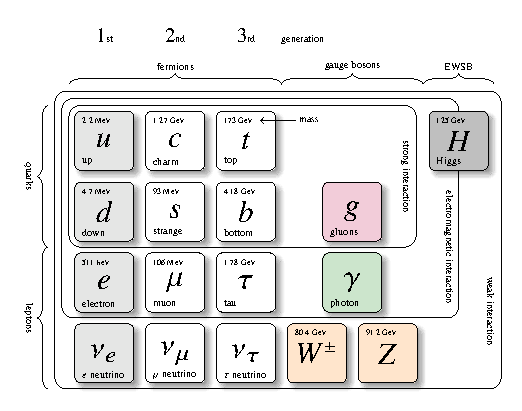
\includegraphics[width=0.75\textwidth,trim=0.9cm 0.3cm 0.2cm 1.5cm,clip]{theory/sm_talk}
      };

      \onslide<2->{%
        \draw[Red,line width=2pt] (-1.65,-1.78) rectangle (-0.1,-0.25);
        \draw[Blue,line width=2pt] (-1.65,-0.05) rectangle (-0.1,1.48);
        \draw[Green,line width=2pt] (3.53,1.67) rectangle (5.08,3.20);
      }

      \node at (3.8,-3.85) {
        \scriptsize Adapted from C.\ Burgard
      };
    \end{tikzpicture}
  \end{center}
\end{frame}

% ------------------------------------------------------------------------------

\begin{frame}{The Standard Model Lagrangian}
  \vspace*{-2.0em}
  \begin{center}
    \begin{tikzpicture}
      \node (lagrangian) at (0,0) {
        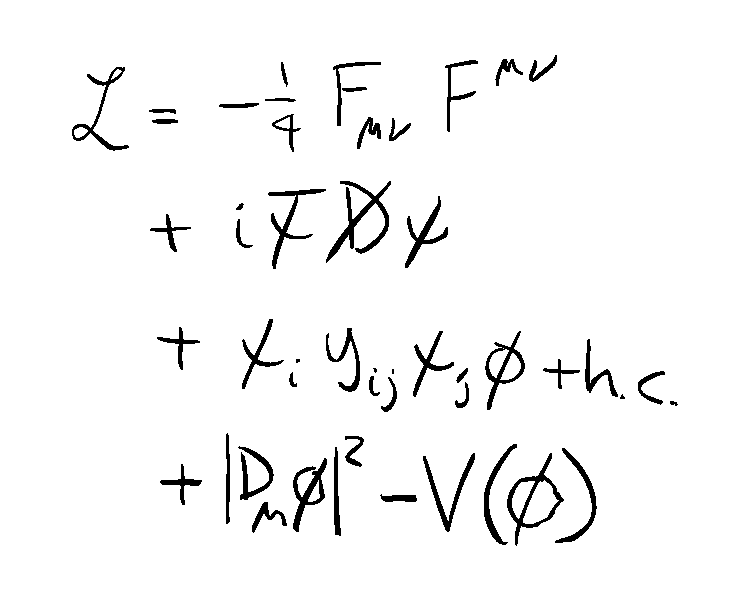
\includegraphics[width=0.6\textwidth]{lagrangian/lagrangian_vectorized}
      };

      \node[anchor=east] (credit) at (3.8,-3.6) {
        \scriptsize Image credit: CERN
      };

      \onslide<1-2>{%
        \path [fill=white] (-4.0,-3.0) rectangle (4,0.0);%
      }

      \onslide<2>{%
        \node[anchor=north west, align=left] at (2.4, 2.1) {%
          \textbf{Local gauge invariance}\\
          $\rightarrow$ Particles must be massless };%
      }

      \pause
      \pause

      \draw[dotted,thick] (-7.4,0.2) -- (7.4,0.2);

      \node[anchor=north west, align=left] at (-7.4,0.1) {%
        \textbf{Higgs sector} (1960s)\\[1.5ex]
        \footnotesize Mass generation through\\[-0.55ex]
        \footnotesize Spontaneous Symmetry\\[-0.55ex]
        \footnotesize Breaking
      };

      \pause

      \draw[Red,thick] (-2.7,-1.4) rectangle (3.8,0);

      \node[anchor=west] at (4.0,-0.7) {%
        \color{Red} Yukawa couplings};

      \draw[Green,thick] (-2.7,-3.0) rectangle (-0.1,-1.5);

      \node[anchor=east] at (0.0,-3.4) {%
        \color{Green}Gauge boson couplings};

      \draw[Blue,thick] (0.0,-3.0) rectangle (2.9,-1.5);

      \node[anchor=west] at (3.0, -2.25) {%
        \color{Blue}Higgs potential
      };
    \end{tikzpicture}
  \end{center}
\end{frame}

% ------------------------------------------------------------------------------

% \begin{frame}{Electroweak Symmetry Breaking}
%   % Brout, Englert, Higgs -> EWSB

%   \begin{columns}[onlytextwidth]
%     \column{0.65\textwidth}

%     Higgs field (weak isospin doublet):
%     \begin{align*}
%       \phi =
%       \begin{pmatrix}
%         \phi^+ \\
%         \phi^0
%       \end{pmatrix}
%       =  \frac{1}{\sqrt{2}}
%       \begin{pmatrix}
%         \phi_1 + i \phi_2\\
%         \phi_3 + i \phi_4
%       \end{pmatrix}
%       \qquad \phi_i \in \mathbb{R}
%     \end{align*}

%     % Add a (doublet) of complex scalar field with a special potential

%     Higgs potential:
%     \begin{align*}
%       V(\phi) = \mu^2 \phi^\dag \phi + \lambda (\phi^\dag \phi)^2
%     \end{align*}

%     % Degenerate minima at:
%     % \begin{align*}
%     %   \sum_{i = 1}^{4} \phi_i^2 = -\frac{\mu^2}{\lambda} \eqqcolon v^2
%     % \end{align*}

%     \column{0.35\textwidth}
%     \centering

%     %\textbf{2D toy model:}

%     \begin{tikzpicture}
%       \node (potential) at (0,0) {%
%         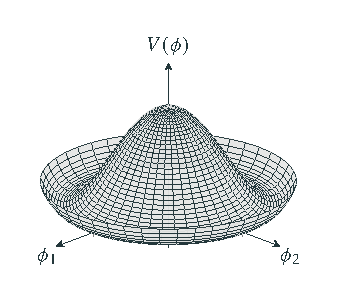
\includegraphics[width=\textwidth, trim=1em 1em 1em 1.5em,
%         clip]{theory/potential}%
%       };

%       \filldraw[color=Red,fill opacity=0.9,draw opacity=0] (0,0.9) circle (3.5pt);

%       \filldraw[color=Red,fill opacity=0.9,draw opacity=0] (-1.8,-0.7) circle (3.5pt);

%       \draw[stealth-, line width=1.2pt, color=Red] (-1.8,-0.55) -- (-1.8,0.7)%
%       node[above]{\footnotesize \textbf{vacuum state}};

%       \draw[stealth-stealth, line width=1.2pt, color=Goldenrod] %
%       (-1.65,-0.7) -- node[midway,below]{\footnotesize \allbold{$v$}} (0,-0.7);
%     \end{tikzpicture}
%   \end{columns}

%   Higgs potential after EWSB in unitary gauge ($H \in \mathbb{R}$):
%   \begin{align*}
%     \phi = \frac{1}{\sqrt{2}}
%     \begin{pmatrix}
%       0 \\
%       v + H
%     \end{pmatrix}
%     \quad \ra \quad
%     V(H) = \underbrace{\lambda v^2}_{m_{H}^2 / 2} H^2 + \lambda v H^3 + \frac{\lambda}{4} H^4
%   \end{align*}
% \end{frame}

% ------------------------------------------------------------------------------

\begin{frame}{Electroweak Symmetry Breaking}
  \begin{center}
    \begin{tikzpicture}
      \node (potential) at (0,0) {%
        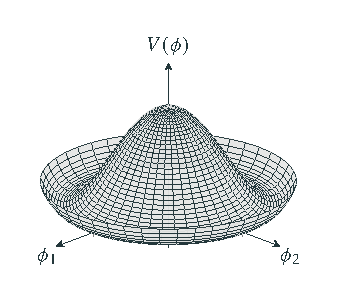
\includegraphics[width=0.4\textwidth, trim=1em 1em 1em 1.5em,
        clip]{theory/potential}%
      };

      \draw[stealth-, line width=1pt] (2.65, -0.5) -- (3.4, -0.5) %
      node[right, align=center]{%
        \footnotesize Higgs potential\\[-0.5ex]
        \footnotesize $V(\phi) = \mu^2 \phi^\dag \phi + \lambda (\phi^\dag \phi)^2$%
      };

      \onslide<2->{
        \filldraw[color=Red,fill opacity=1.0,draw opacity=0] (0,1.05) circle (3.5pt);

        \draw[stealth-, line width=1pt] (0.25, 1.05) -- (2, 1.05) %
        node[right, align=center]{%
          \footnotesize symmetric state%
        };
      }

      \onslide<3->{
        \filldraw[color=Red,fill opacity=1.0,draw opacity=0] (-2.1,-0.8) circle (3.5pt);

        \draw[stealth-, line width=1pt, color=Red] (-2.15,-0.6) -- (-2.8,0.8)%
        node[above, align=center]{%
          \footnotesize vacuum state\\[-0.5ex]
          \footnotesize \color{headergray} broken symmetry\\[-0.5ex]
          \footnotesize \color{headergray} ($m_{W,Z} \neq 0$, $m_\gamma = 0$)%
        };

        \draw[stealth-stealth, line width=1pt, color=Red] %
        (-1.95,-0.8) -- node[midway,below]{$\mathbf{v}$\,\,} (0,-0.8);%

        \node[anchor=east] at (-3.3,-0.75) {%
          \footnotesize $\displaystyle v = \frac{\lvert \mu \rvert}{\sqrt{\lambda}}$};%
      }
    \end{tikzpicture}
  \end{center}

  % \vspace*{-1em}

  % \onslide<4->{
  %   \textbf{Perturbation theory:} Consider small perturbations about the vacuum state
  %   \begin{itemize}
  %   \item Radial perturbations \ra Physical Higgs boson
  %     $m_{H} = \sqrt{2 \lambda} v$
  %   \item Angular perturbations \ra Nambu--Goldstone bosons
  %   \end{itemize}
  % }
\end{frame}

% ------------------------------------------------------------------------------

{ % all template changes are local to this group.
  \setbeamertemplate{navigation symbols}{}
  \setbeamercolor{background canvas}{bg=black}
  \begin{frame}<article:0>[plain]
    \setlength{\fboxrule}{1pt}
    \begin{tikzpicture}[remember picture,overlay,shift=(current page.south
      west),x=(current page.south east),y=(current page.north west)]

      \node[at=(current page.center)] { 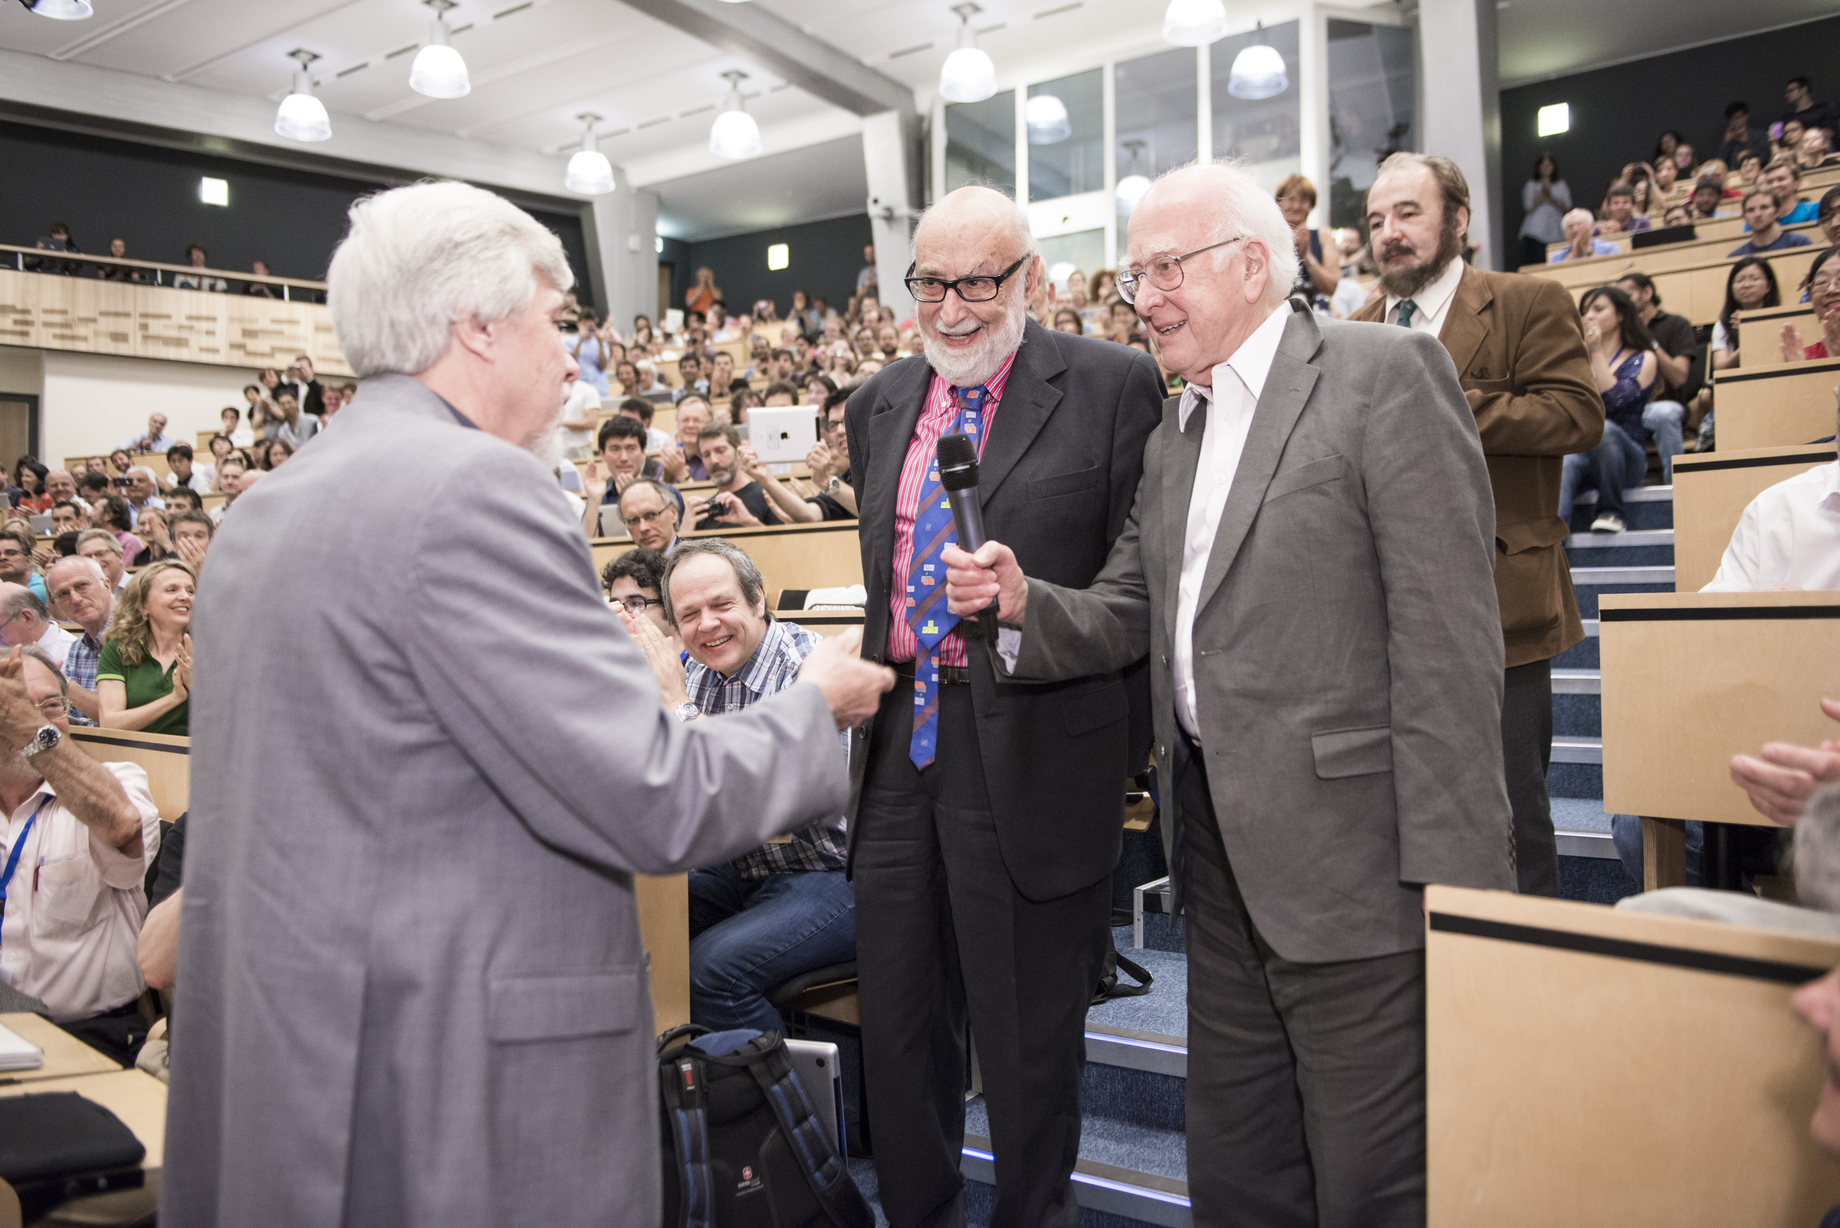
\includegraphics[keepaspectratio,
        width=\paperwidth, height=\paperheight, trim=0 2.05cm 0 0,
        clip]{CERN_seminar_25pct} };

      % \node[align=center] at (0.2,0.27){%
      %   \fcolorbox{headergray}{white}{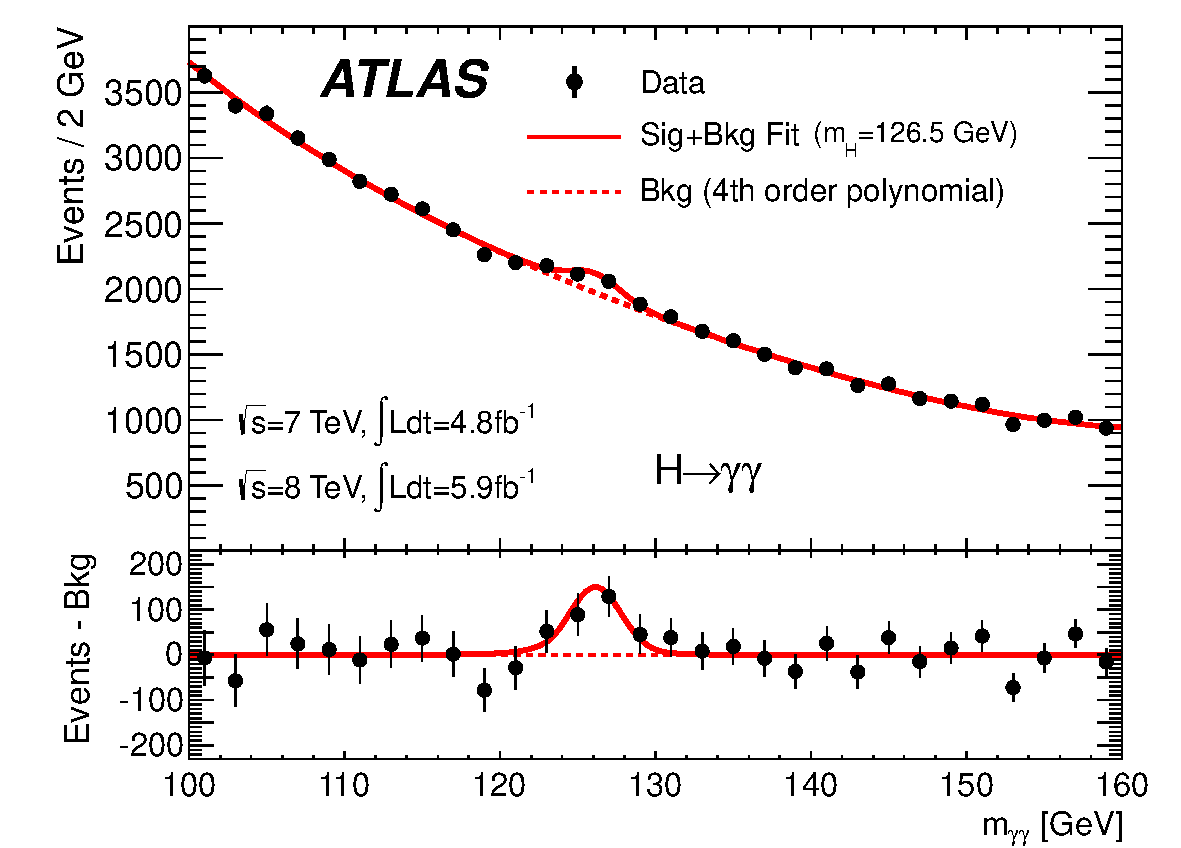
\includegraphics[width=0.36\textwidth]{higgs_discovery/figaux_004a}}
      % };

      \node[align=center] at (0.21,0.27){%
        \fcolorbox{headergray}{white}{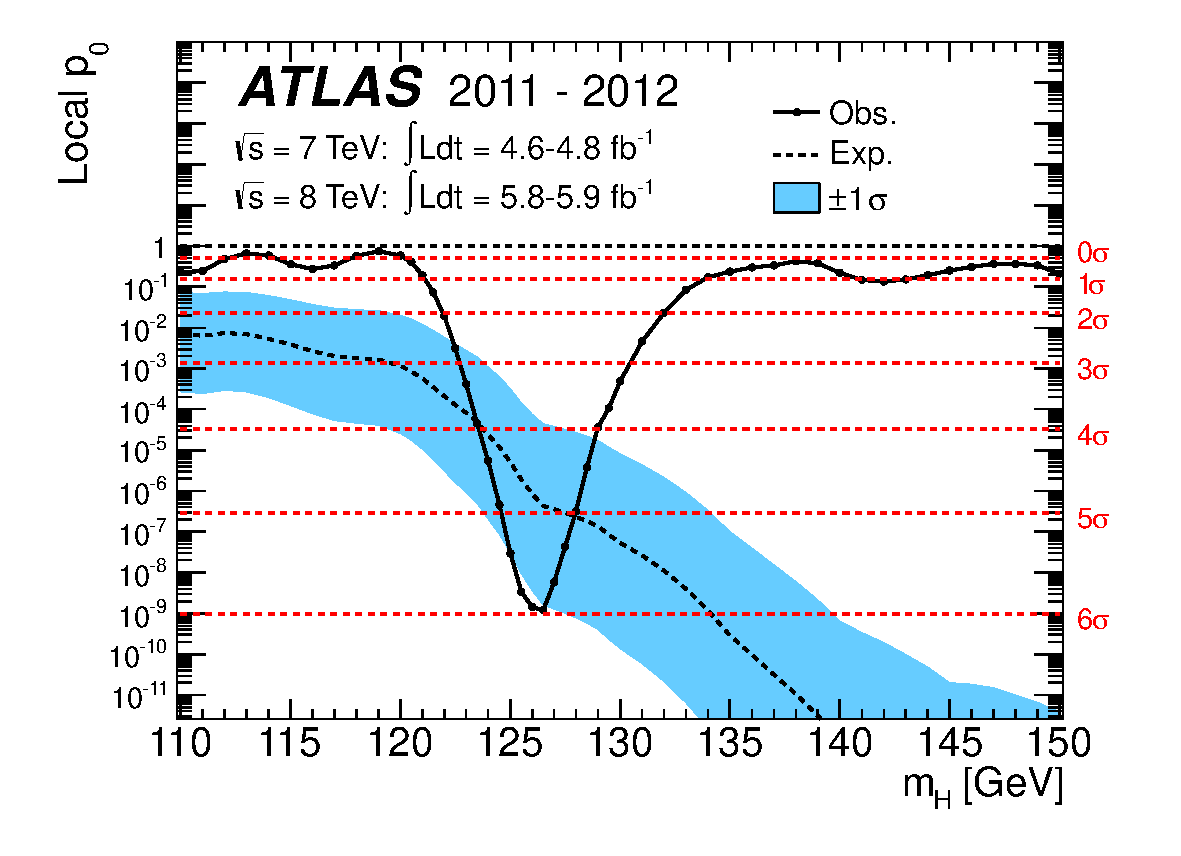
\includegraphics[width=0.42\textwidth]{higgs_discovery/fig_009}}
      };

      % \node[align=center] at (0.85, 0.27){%
      %   \fcolorbox{headergray}{white}{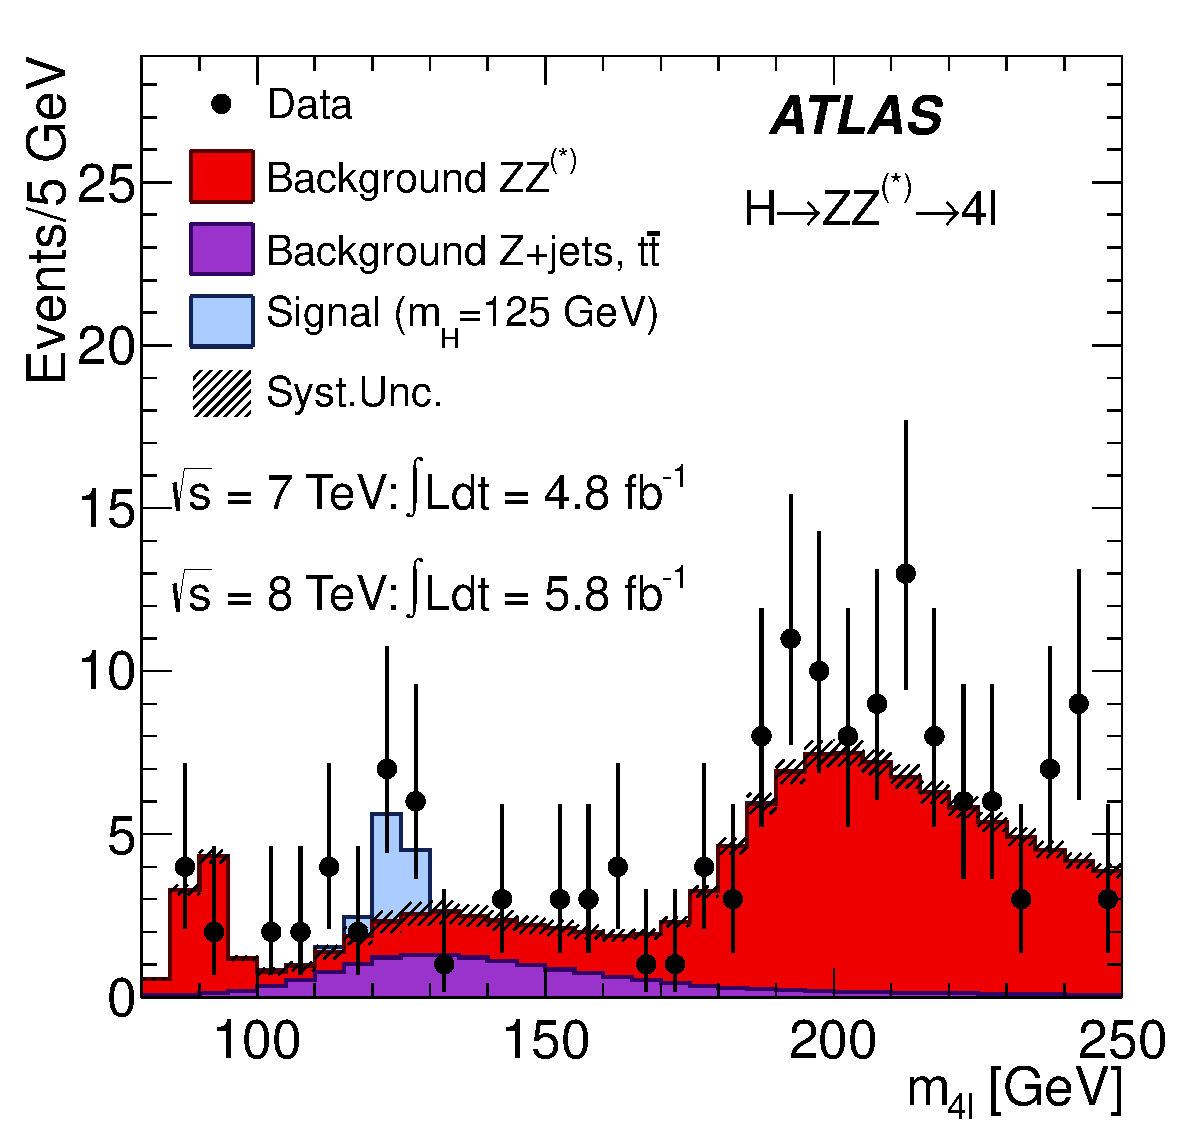
\includegraphics[width=0.27\textwidth]{higgs_discovery/fig_002}}
      % };

      \node[anchor=east] at (1.0, 0.93){%
        \fcolorbox{headergray}{white}{
          \begin{minipage}{0.35\textwidth}
            CERN seminar (July 4, 2012)\\[-0.5em]
            {\tiny Credit:~CERN (photo), HIGG-2012-27 (plot)}
          \end{minipage}
        }
      };

      % \node[align=center] at (0.55,0.15){%
      %   \fcolorbox{headergray}{white}{$m_{H} \approx \SI{125}{\GeV}$};
      % };

      \node[align=center] at (0.165,0.133){%
        \textcolor{black}{$m_{H} \approx \SI{125}{\GeV}$}
      };
    \end{tikzpicture}
  \end{frame}
}


% ------------------------------------------------------------------------------

\begin{frame}{The Higgs Boson Self-Coupling}
  Higgs potential after symmetry breaking:
  \begin{center}
    \begin{tabular}{ccccccc}
      $V(H)$ & $=$ & ${\color{Red} \lambda v^2 H^2}$ & $+$ & ${\color{Blue} \lambda v H^3}$ & $+$ & ${\color{Green} \frac{\lambda}{4} H^4}$ \\[1.2em]
             && \onslide<2->{\raisebox{1.85em}{
\includegraphics[scale=1.0]{feynman_graphs_talk/higgs_massterm}}}
             && \onslide<3->{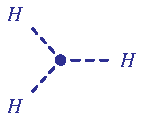
\includegraphics[scale=1.0]{feynman_graphs_talk/higgs_hhh}}
             && \onslide<4->{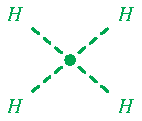
\includegraphics[scale=1.0]{feynman_graphs_talk/higgs_hhhh}} \\[1.2em]
             && \onslide<2->{\color{Red}mass term}
             && \onslide<3->{\color{Blue}trilinear self-coupling}
             && \onslide<4->{\color{Green}quartic self-coupling} \\[1.5em]
             && \onslide<2->{\color{Red}\checkmark}
             && \onslide<3->{\color{Blue}?}
             && \onslide<4->{\color{Green}?}
    \end{tabular}
  \end{center}

  % \onslide<5->{%
  %   \setlength{\fboxrule}{1pt}
  %   \begin{tikzpicture}[remember picture,overlay,shift=(current page.south
  %     west),x=(current page.south east),y=(current page.north west)]

  %     \filldraw[white,opacity=0.7](0.0,0.15) rectangle (1.0,0.85);

  %     \node[align=center] at (0.5,0.5){%
  %       \fcolorbox{headergray}{white}{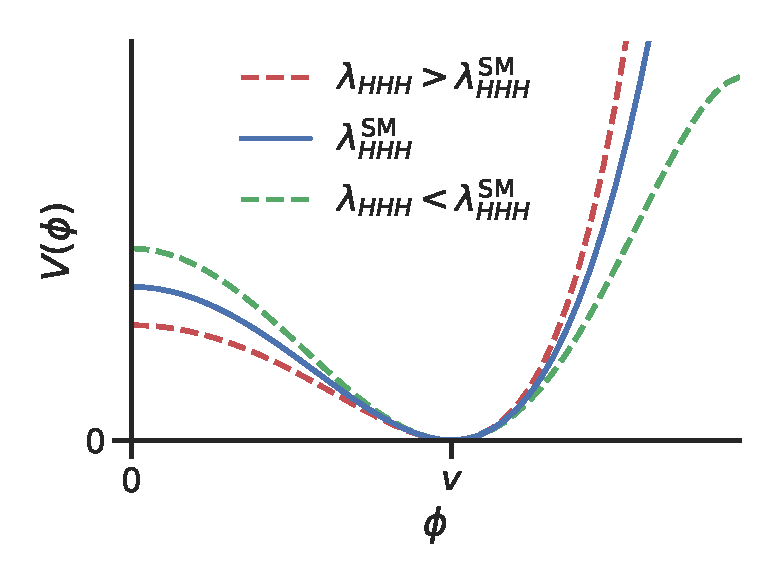
\includegraphics[width=0.5\textwidth]{higgs_potential_variation}}
  %     };

  %     \node[align=center] at (0.542,0.42){%
  %       \huge ?
  %     };
  %   \end{tikzpicture}
  % }
\end{frame}

% ------------------------------------------------------------------------------

\begin{frame}{Higgs Boson Pair Production in the SM}
  \vspace*{0.5em}

  \textbf{Dominant production mode:}

  \vspace*{0.5em}

  \fbox{%
    \noindent\begin{minipage}{\dimexpr 0.25\textwidth - 2\fboxsep}
      \centering
      \textbf{Gluon--gluon fusion}\\[0.5\baselineskip]
      $\sigma_{\HH}^{gg\text{F}} = \SI{31}{\femto\barn}$
  \end{minipage}%
  \begin{minipage}{\dimexpr 0.75\textwidth - 2\fboxsep}
    \vspace*{0.5em}

    \hspace*{0.05\textwidth}
    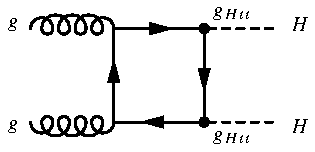
\includegraphics[scale=0.85]{feynman_graphs/di_higgs_box}%
    \hfill%
    \raisebox{0.35em}{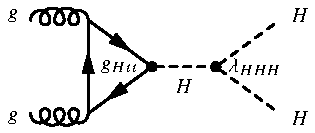
\includegraphics[scale=0.85]{feynman_graphs/di_higgs_triangle}}%
    \hspace*{0.05\textwidth}

    \vspace*{0.5em}
  \end{minipage}
  }

  % \vspace*{2em}

  % \onslide<2->{%
  % \fbox{%
  %   \noindent\begin{minipage}{\dimexpr 0.25\textwidth - 2\fboxsep}
  %     \centering
  %     \textbf{Vector boson fusion}\\[0.5\baselineskip]
  %     $\sigma_{\HH}^{\text{VBF}} = \SI{1.7}{\femto\barn}$
  %   \end{minipage}%
  %   \begin{minipage}{\dimexpr 0.75\textwidth - 2\fboxsep}
  %     \hspace*{0.04\textwidth}%
  %     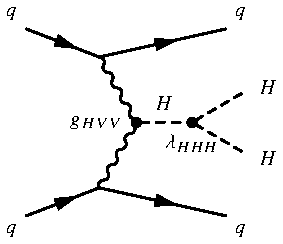
\includegraphics[width=0.3\textwidth]{feynman_graphs/di_higgs_vbf_kvklam}%
  %     \hfill%
  %     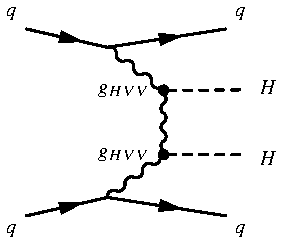
\includegraphics[width=0.3\textwidth]{feynman_graphs/di_higgs_vbf_kvkv}%
  %     \hfill%
  %     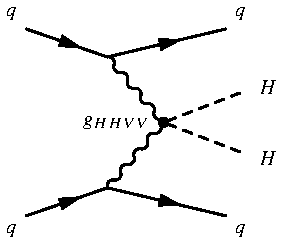
\includegraphics[width=0.3\textwidth]{feynman_graphs/di_higgs_vbf_ktwov}%
  %     \hspace*{0.04\textwidth}
  %   \end{minipage}
  % }
  % }

  \vspace*{1.0em}
  {\scriptsize In $pp$ collisions at $\sqrt{s} = \SI{13}{\TeV}$}
\end{frame}




% ------------------------------------------------------------------------------

\begin{frame}{The ATLAS Experiment at the LHC}
  \centering

  \only<1>{%
    \begin{overpic}[scale=0.95]{lhc_atlas/lhc_atlas_1}
      \put(0,52){Run~2 (2015--2018)}
      \put(0,48){$\sqrt{s} = \SI{13}{\TeV}$}
    \end{overpic}
  }
  \only<2>{%
    \begin{overpic}[scale=0.95]{lhc_atlas/lhc_atlas_2}
      \put(0,52){Run~2 (2015--2018)}
      \put(0,48){$\sqrt{s} = \SI{13}{\TeV}$}
      \put(23.5,52){$\int L \, \text{d}t = \SI{139}{\per\femto\barn}$}
    \end{overpic}
  }
\end{frame}

% ------------------------------------------------------------------------------

\begin{frame}{Final States of Searches for \allbold{\HH} Production}
  \begin{columns}[onlytextwidth]
    \column{0.5\textwidth}

    \textbf{Most promising
      channels (SM):}\\
    $b\bar{b}b\bar{b}$, \bbtautau, $b\bar{b}\gamma\gamma$
    \begin{itemize}
    \item Trade-off between branching ratio \& ``cleanliness'' of final state
    \end{itemize}

    \column{0.5\textwidth}
    \centering

    \allbold{\small $HH$-system branching ratios:}

    \vspace*{0.5em}

    \begin{overpic}[width=0.9\textwidth]{theory/di_higgs_branching_ratio}
      \put(29.5, 51.7){\Large $\color{white}{\star}$}
      \put(29.5, 29.6){\Large $\color{black}{\star}$}
      \put(29.5, 7.4){\Large $\color{black}{\star}$}
    \end{overpic}
  \end{columns}
\end{frame}

% ------------------------------------------------------------------------------

\begin{frame}{The \allbold{\bbtautau} Final State}

  \begin{columns}[onlytextwidth]
    \column{0.4\textwidth}

    % \textbf{Advantages:}
    % \begin{itemize}
    %   \setlength{\itemsep}{0.5em}
    % \item Large $H \to b\bar{b}$ branching ratio
    % \item Distinct signature of $H \to \tau^+\tau^-$
    % \end{itemize}

    % \vspace{1em}
    % \pause

    \textbf{Channels:}
    \begin{itemize}
      \setlength{\itemsep}{0.5em}
    \item<1-> \lephad channel\\
      $\mathcal{B}(\tau^+\tau^- \to \lephad) \approx \SI{45.6}{\percent}$

    \item<2-> \hadhad channel\\
      $\mathcal{B}(\tau^+\tau^- \to \hadhad) \approx \SI{42.0}{\percent}$
    \end{itemize}

    \column{0.6\textwidth} \centering
    % \begin{overlayarea}{\textwidth}{0.5cm}
    %   \centering
    %   \only<1>{\lephad}%
    %   \only<2>{\hadhad}
    % \end{overlayarea}

    \hspace*{0.03\textwidth}%
    \only<1>{\vspace*{-1pt}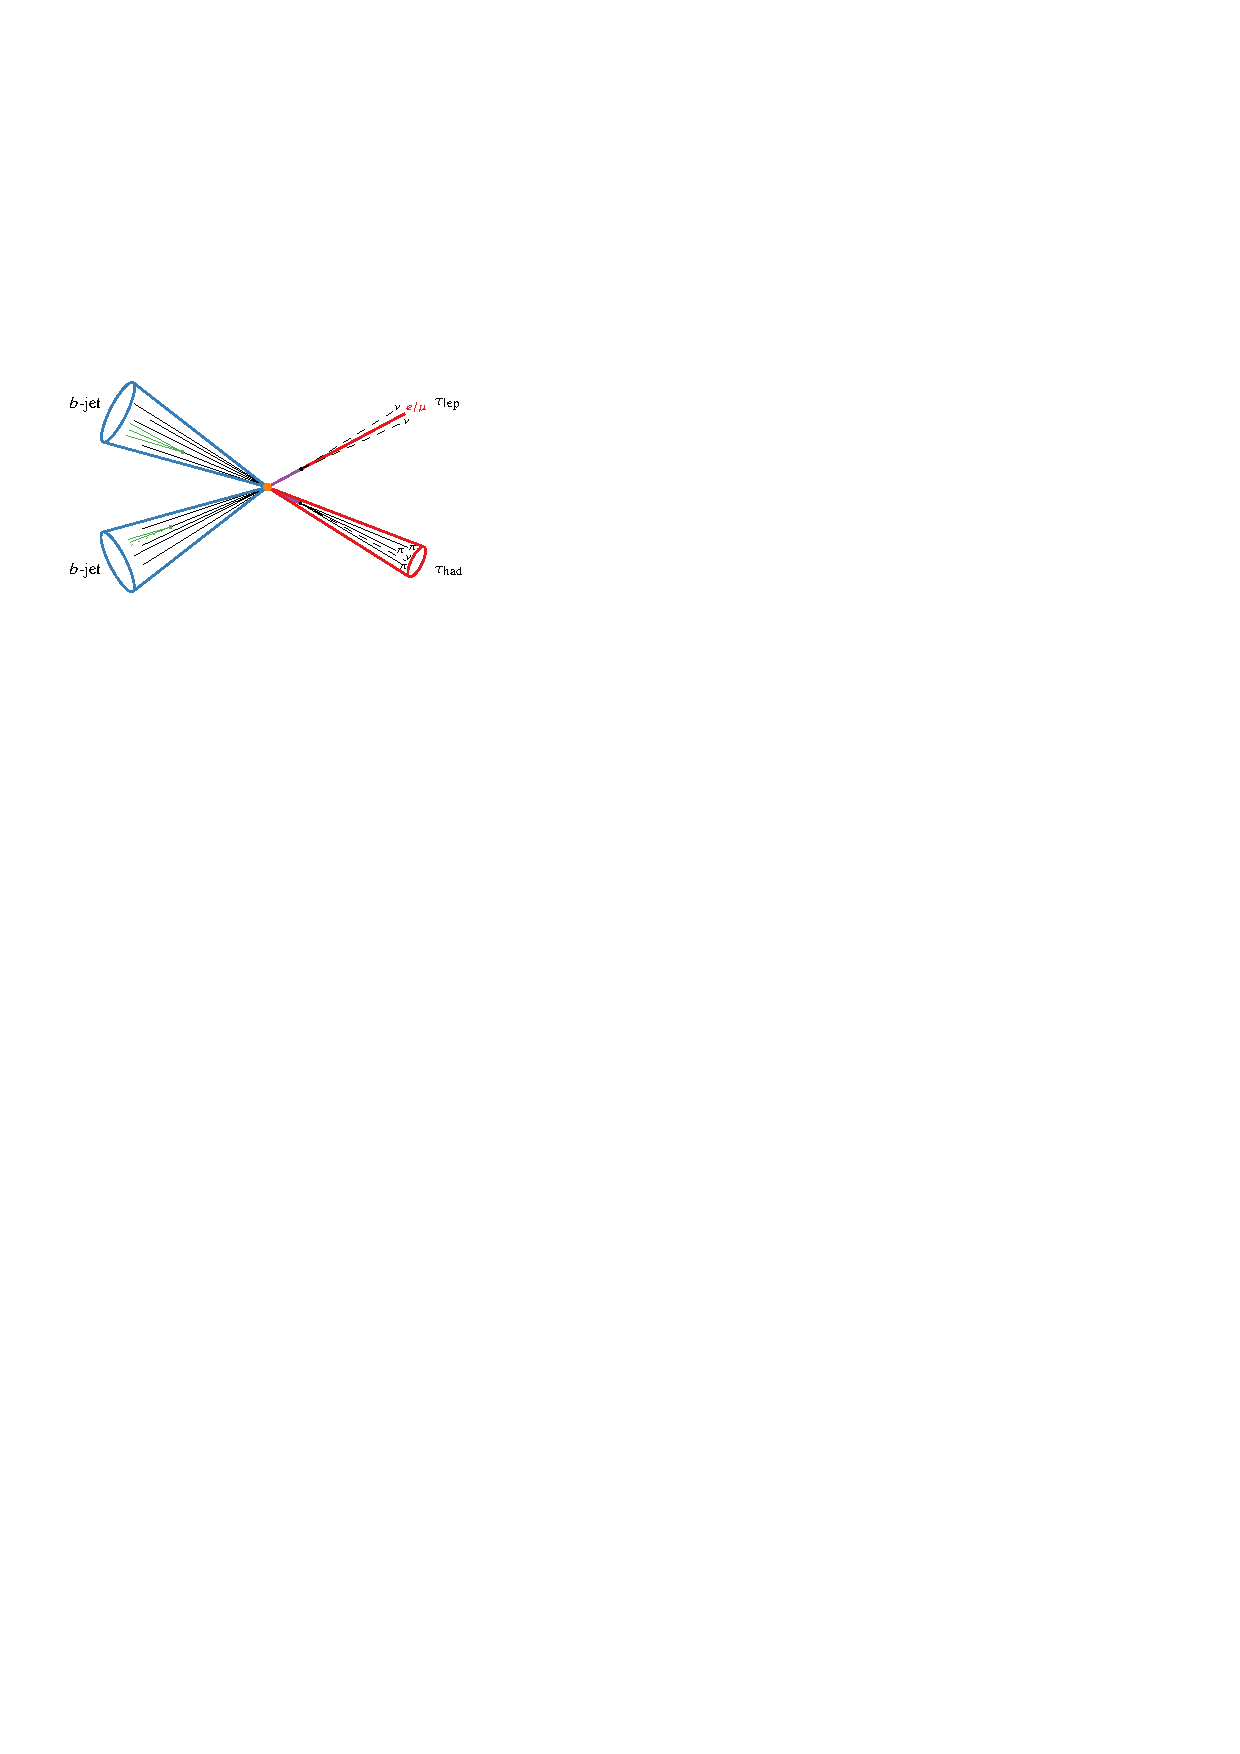
\includegraphics[width=0.97\textwidth]{final_state/final_state_lephad}}%
    \only<2>{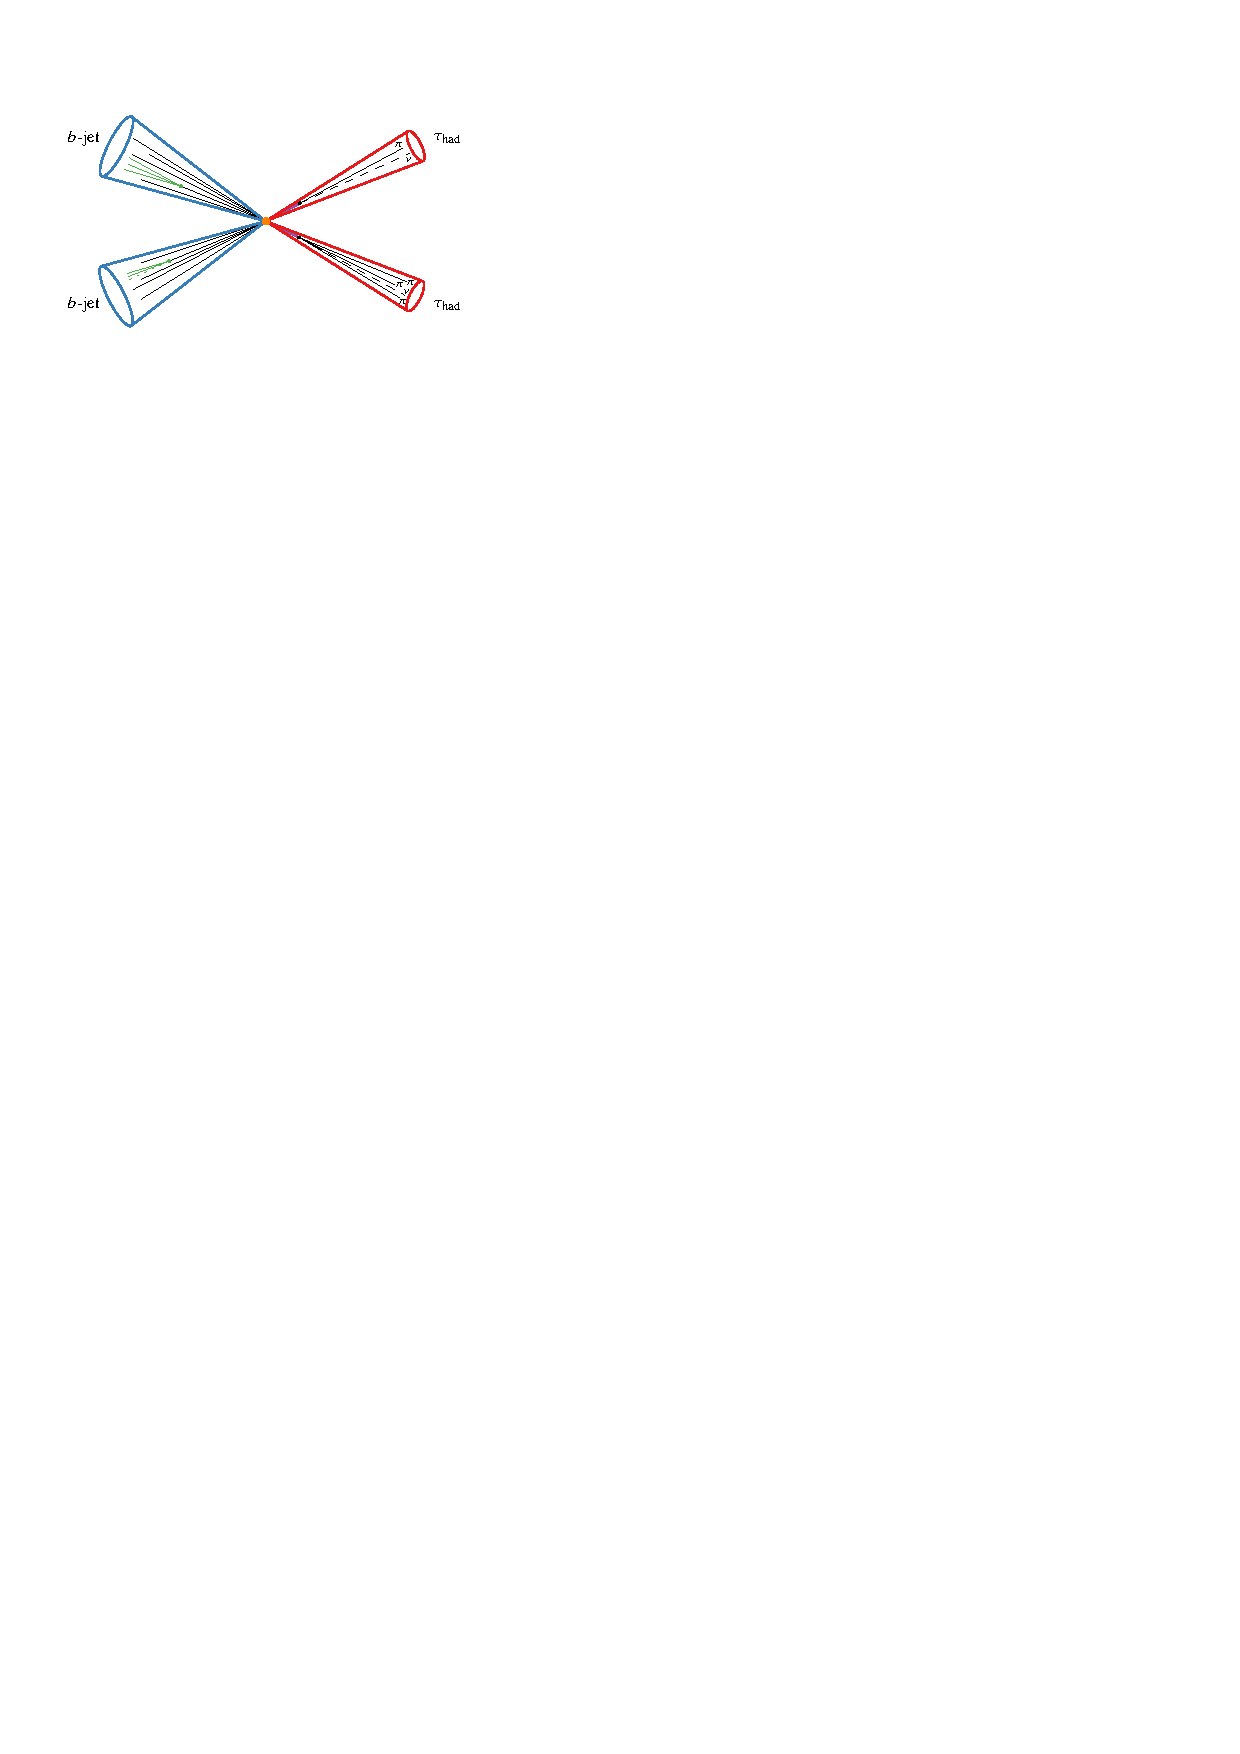
\includegraphics[width=0.97\textwidth]{final_state/final_state_hadhad}}
  \end{columns}
\end{frame}

% ------------------------------------------------------------------------------

\begin{frame}[standout]
  Tau Identification
\end{frame}

% ------------------------------------------------------------------------------

\begin{frame}{Tau Identification}
  \vspace*{1em}

  \begin{columns}
    \column{0.45\textwidth} \centering
    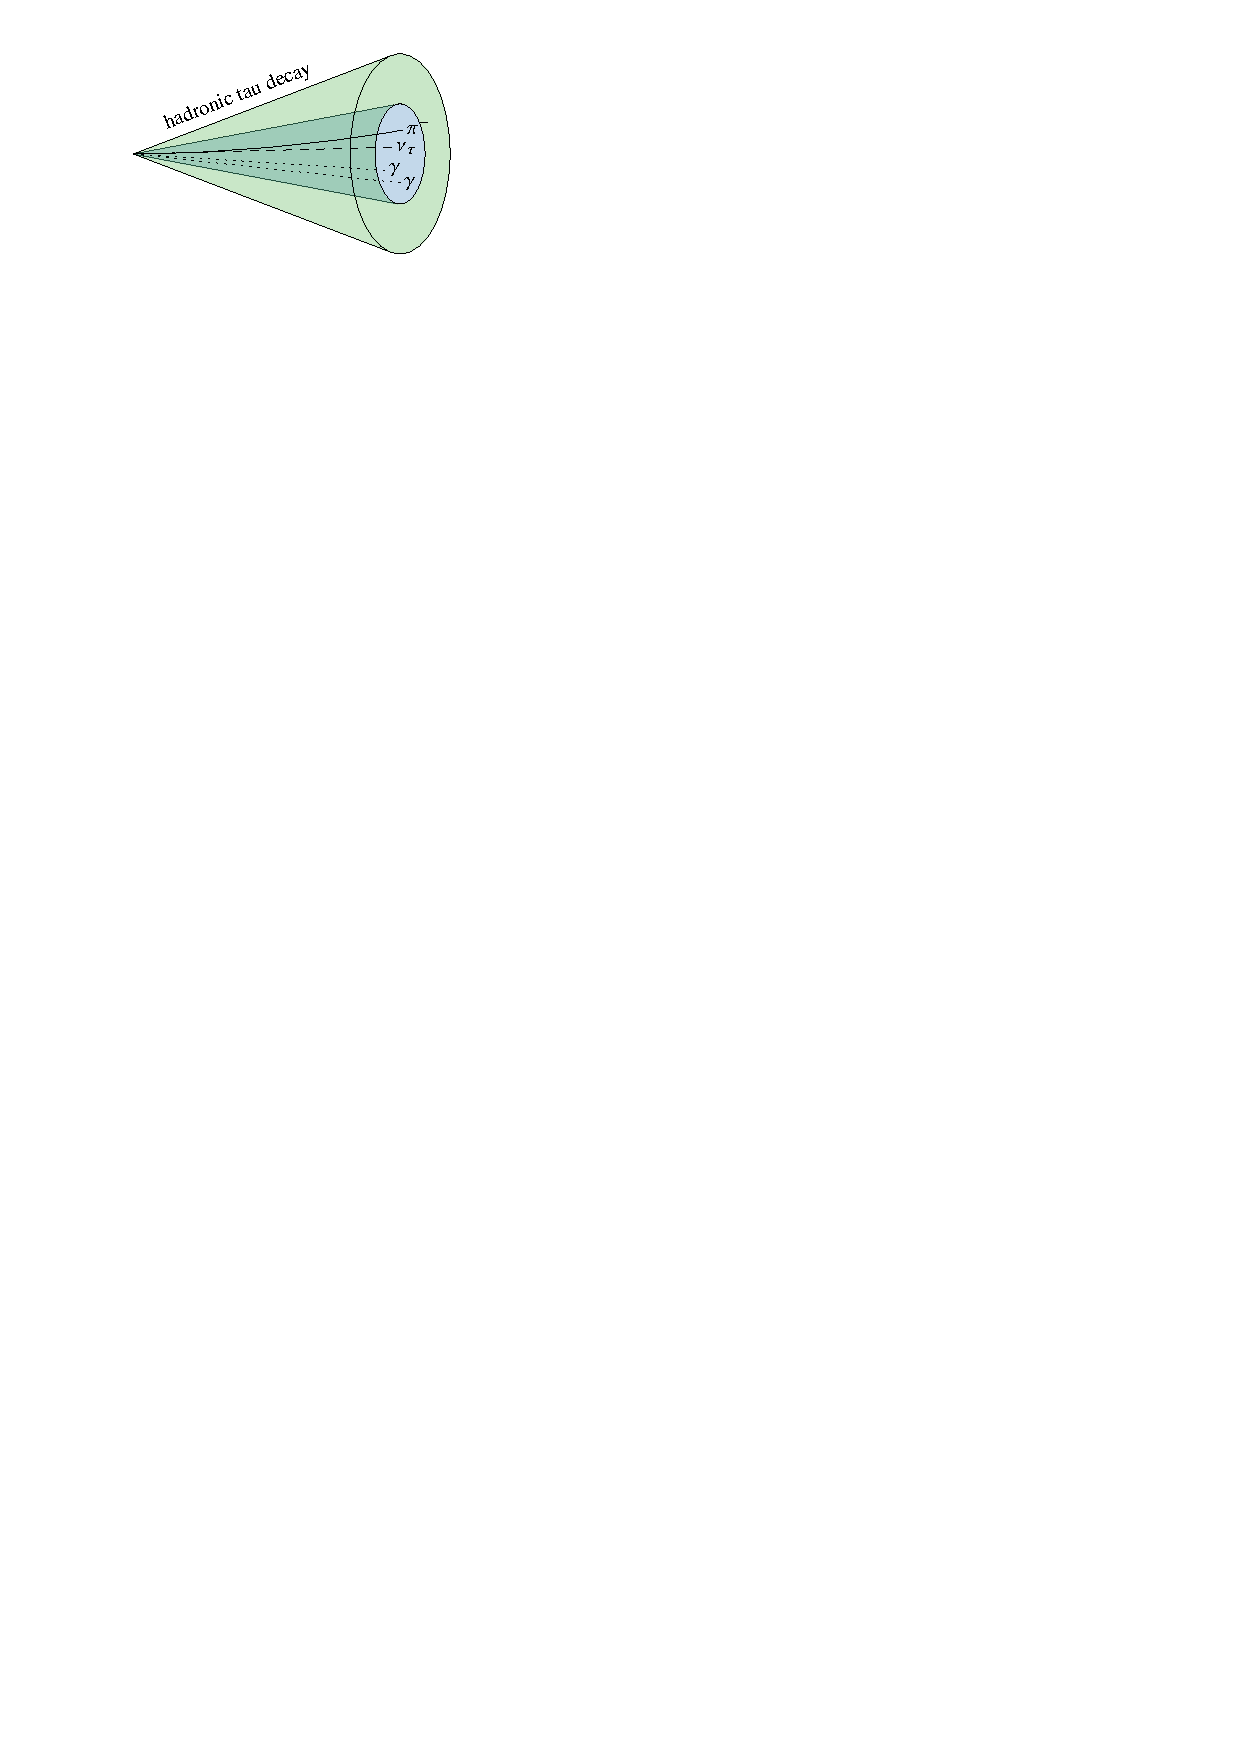
\includegraphics[width=0.75\textwidth]{tauid/cone_tauhad}

    \column{0.10\textwidth}
    \centering

    vs.

    \column{0.45\textwidth}
    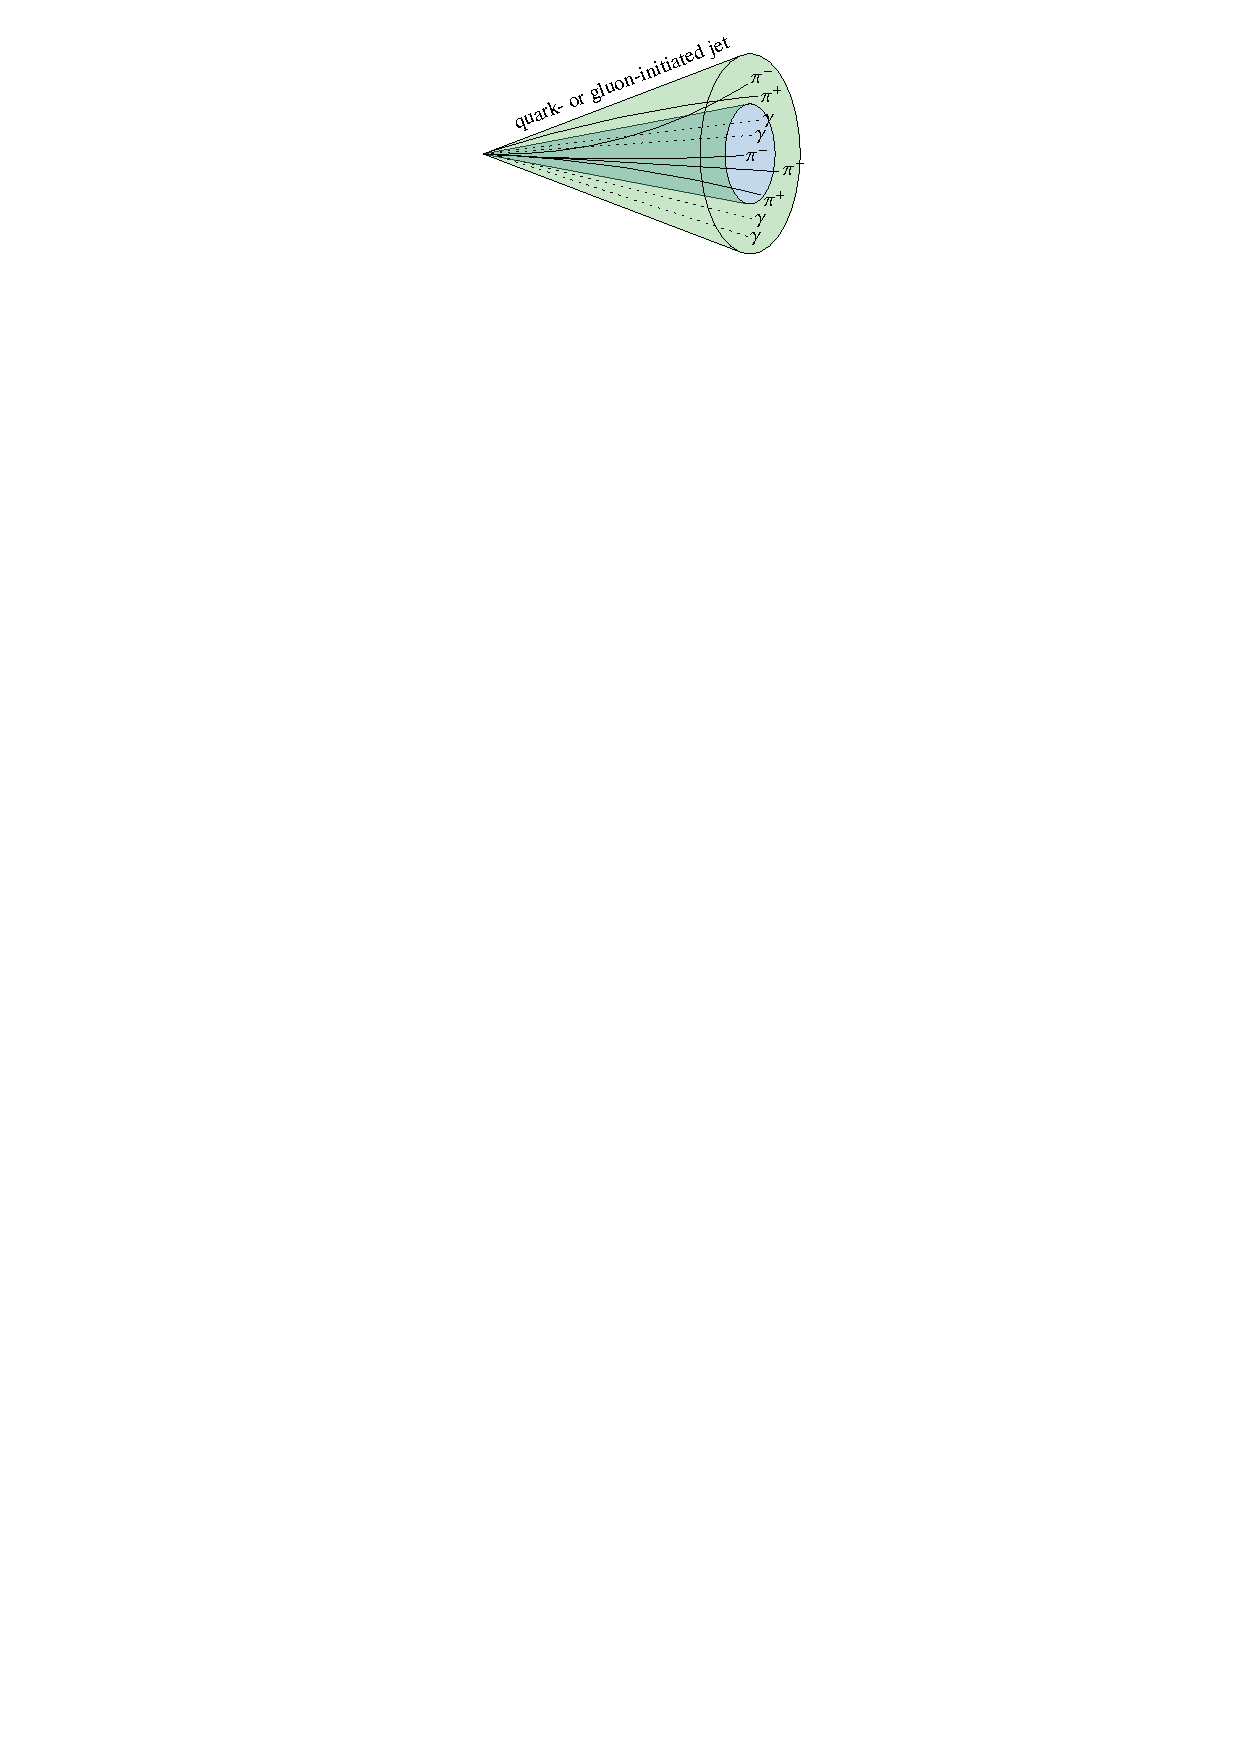
\includegraphics[width=0.75\textwidth]{tauid/cone_qgjet}
  \end{columns}

  \vspace*{0.5em}

  \textbf{Characteristic features:}%

  \begin{columns}[onlytextwidth]
    \column{0.5\textwidth}

    \begin{itemize}
    \item Particle multiplicity
    \item $\tau$ lepton mass ($m_\tau \approx \SI{1.78}{\GeV}$)
    \end{itemize}

    \column{0.5\textwidth}

    \begin{itemize}
    \item Isolation
    \item $\tau$ lepton lifetime ($c\tau \approx \SI{87}{\micro\meter}$)
    \end{itemize}
  \end{columns}

  \vspace*{1.25em}

  \textbf{\ra Classification problem:\ use machine learning techniques}

  % \onslide<2->{%
  %   \tikz[overlay, remember picture, shift=(current page.south west), x=(current
  %   page.south east), y=(current page.north west), ]{ \node[align=center] at
  %     (0.5,0.678) {%
  %       \setlength{\fboxrule}{1pt}%
  %       \fcolorbox{headergray}{mygray}{%
  %         \begin{minipage}{0.75\textwidth}
  %           \centering \vspace*{0.6em} \textbf{Machine learning techniques}

  %           Simulated $\gamma^* \rightarrow \tauhad \tauhad$ for ``signal''

  %           Simulated di-jet events for ``background'' \vspace*{0.6em}
  %         \end{minipage}
  %       }
  %     };
  %   }
  % }
  %     % Optional help grid lines \draw[step=.1, opacity=0.3, thick, red] (0,0)
  %     % grid (1,1); }}
\end{frame}

% ------------------------------------------------------------------------------

\begin{frame}{Tau Identification:\ Input Variables}

  \begin{minipage}[c][2.2cm][c]{0.25\textwidth}
    \centering

    
\includegraphics[scale=1]{tauid/high_level_icon}
  \end{minipage}%
  \begin{minipage}[c][2.2cm][c]{0.75\textwidth}
    Purposefully engineered features\\[0.5\baselineskip]
    \textbf{Inputs:}\ invariant masses, isolation variables, \dots
  \end{minipage}%

  % ---
  \pause
  % ---

  \begin{minipage}[c][2.2cm][c]{0.25\textwidth}
    \centering

    
\includegraphics[scale=1]{tauid/track_icon}
  \end{minipage}%
  \begin{minipage}[c][2.2cm][c]{0.75\textwidth}
    Tracks associated to the \tauhadvis\\[0.5\baselineskip]
    % within $\dR < 0.4$ of \tauhadvis axis\\[0.5\baselineskip]
    \textbf{Inputs:}\ $\pT$, $\Delta \phi$, $\Delta \eta$, impact parameters,
    \dots
  \end{minipage}%

  % ---

  \begin{minipage}[c][2.2cm][c]{0.25\textwidth}
    \centering

    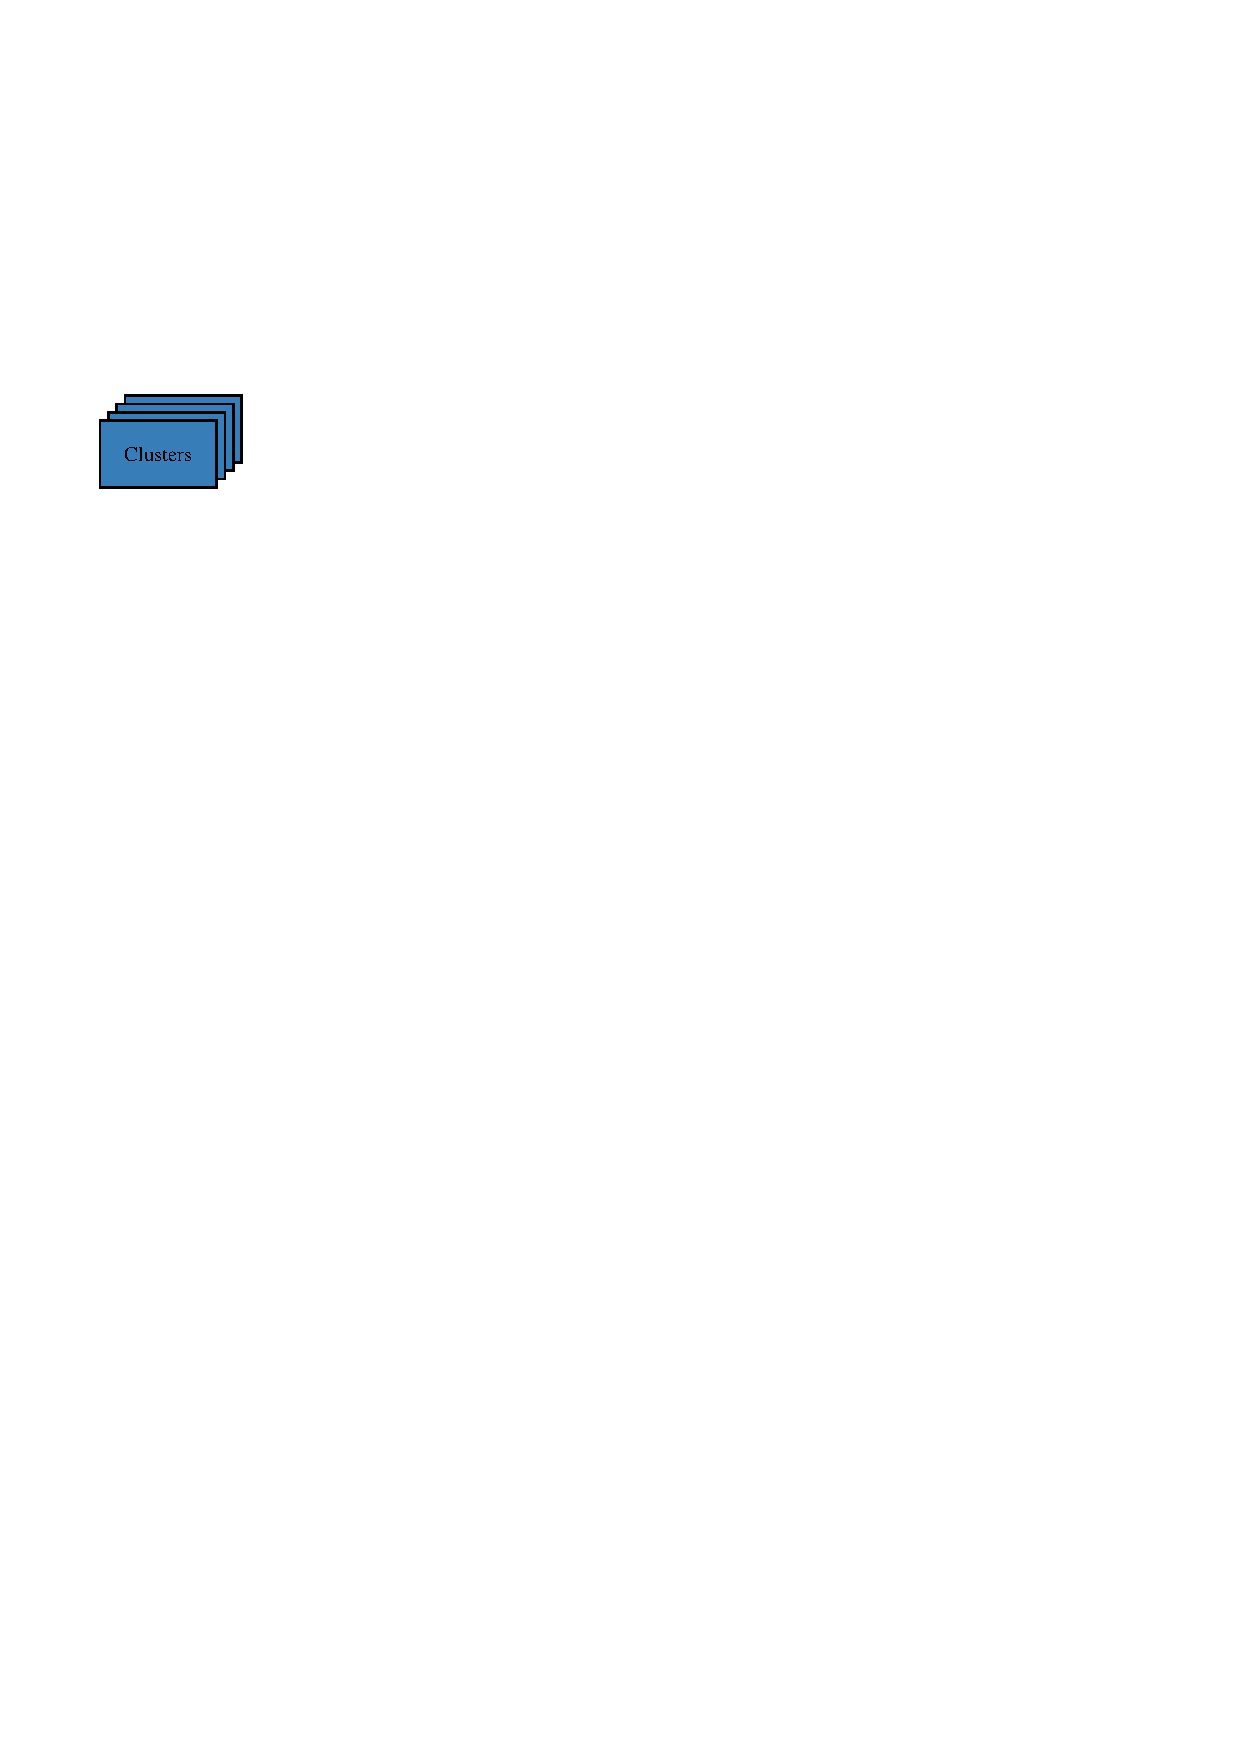
\includegraphics[scale=1]{tauid/cluster_icon}
  \end{minipage}%
  \begin{minipage}[c][2.2cm][c]{0.75\textwidth}
    % Clusters associated to jet seeding the \tauhadvis\\[0.5\baselineskip]
    Clusters associated to the \tauhadvis\\[0.5\baselineskip]
    \textbf{Inputs:}\ $\ET$, $\Delta \phi$, $\Delta \eta$, geometrical cluster
    moments
  \end{minipage}
\end{frame}

% ------------------------------------------------------------------------------

% 4. slide: How does it look in the grand scheme?

% \begin{frame}{Tau Identification: High-Level Variables}
%   \begin{columns}[onlytextwidth]
%     \column{0.25\textwidth} \centering

%     
\includegraphics[scale=1]{tauid/high_level_icon}

%     \column{0.75\textwidth}

%     \begin{columns}[onlytextwidth]
%       \column{0.5\textwidth}
%       \centering

%       $p_{\text{T}}$-fraction of \emph{isolation} tracks\\[0.2em]

%       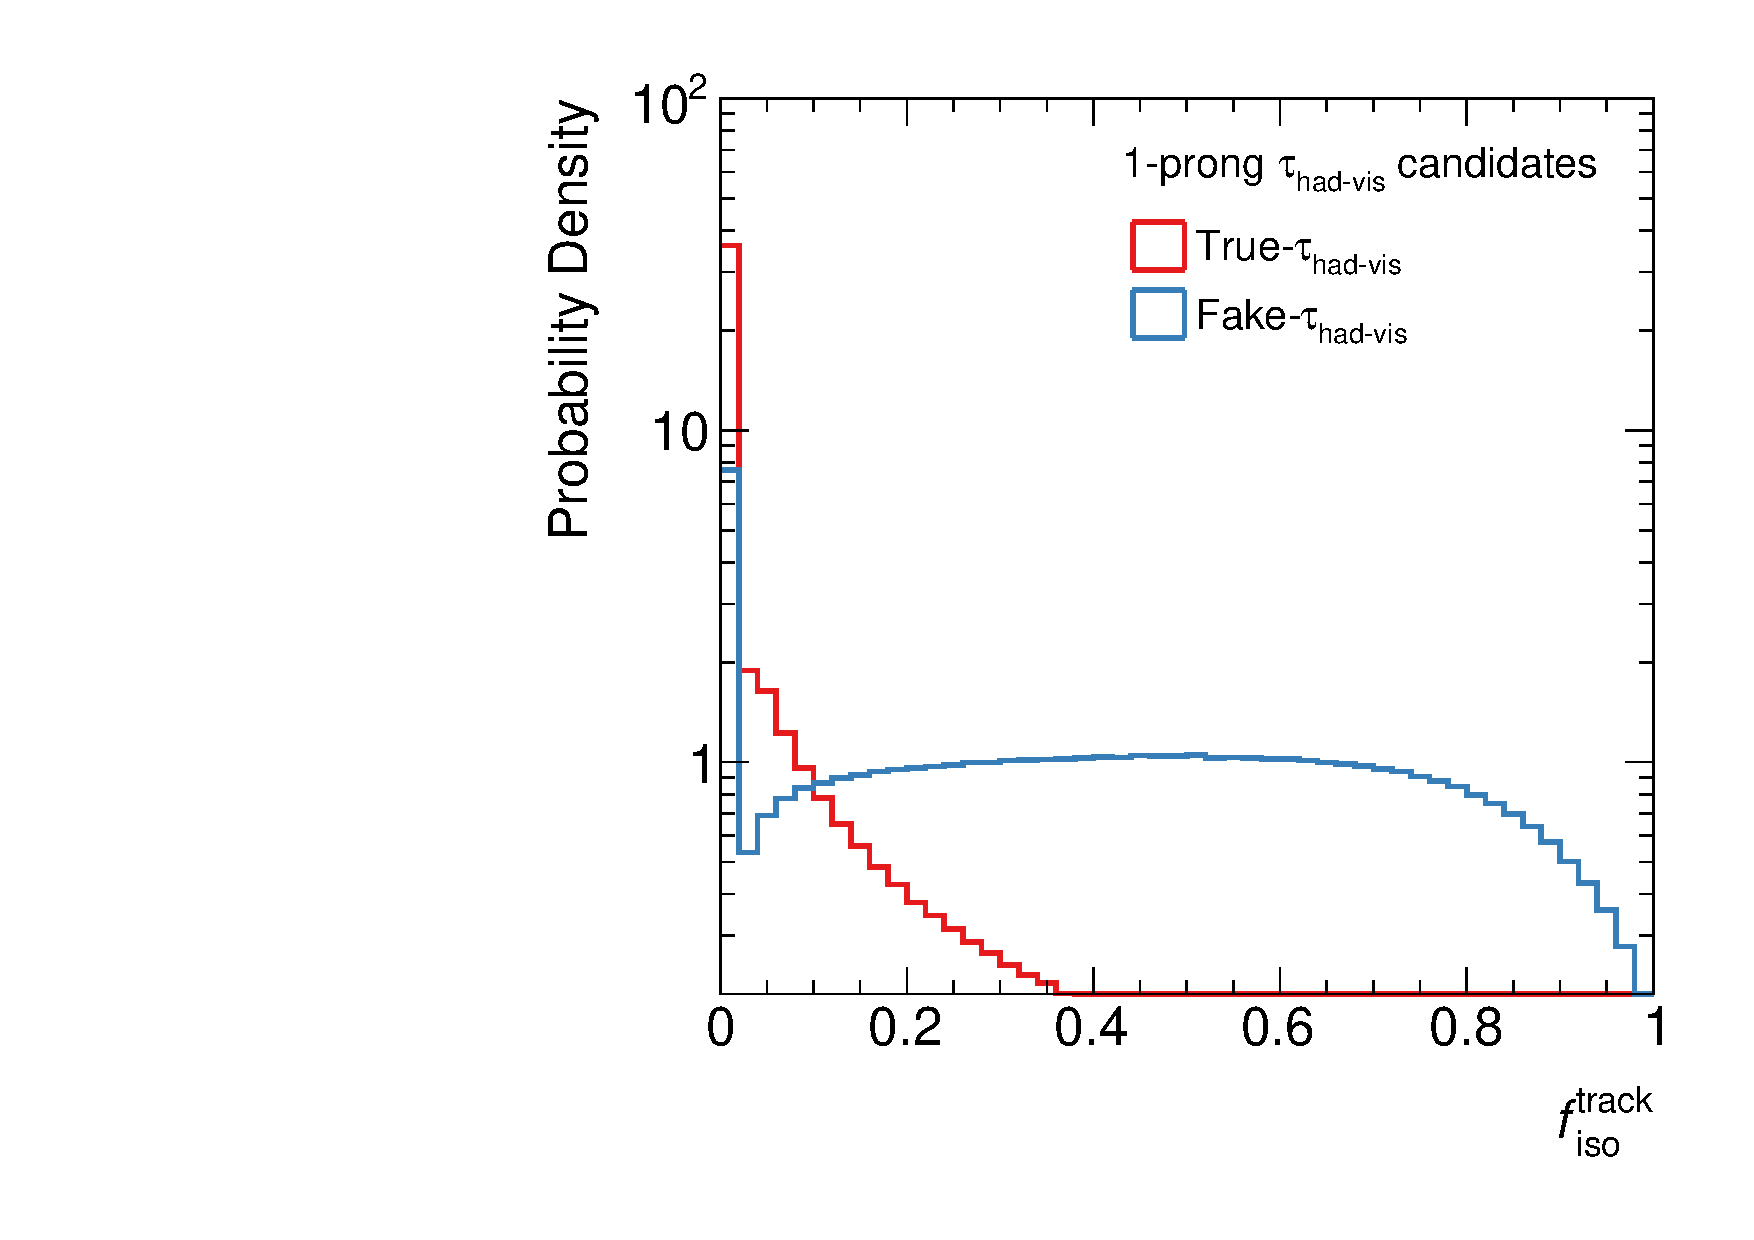
\includegraphics[width=0.9\textwidth]{tauid/invars/invars_sumpttrkfrac_1P}

%       \column{0.5\textwidth}
%       \centering

%       \only{Invariant mass of \emph{core} tracks\\[0.2em]}

%       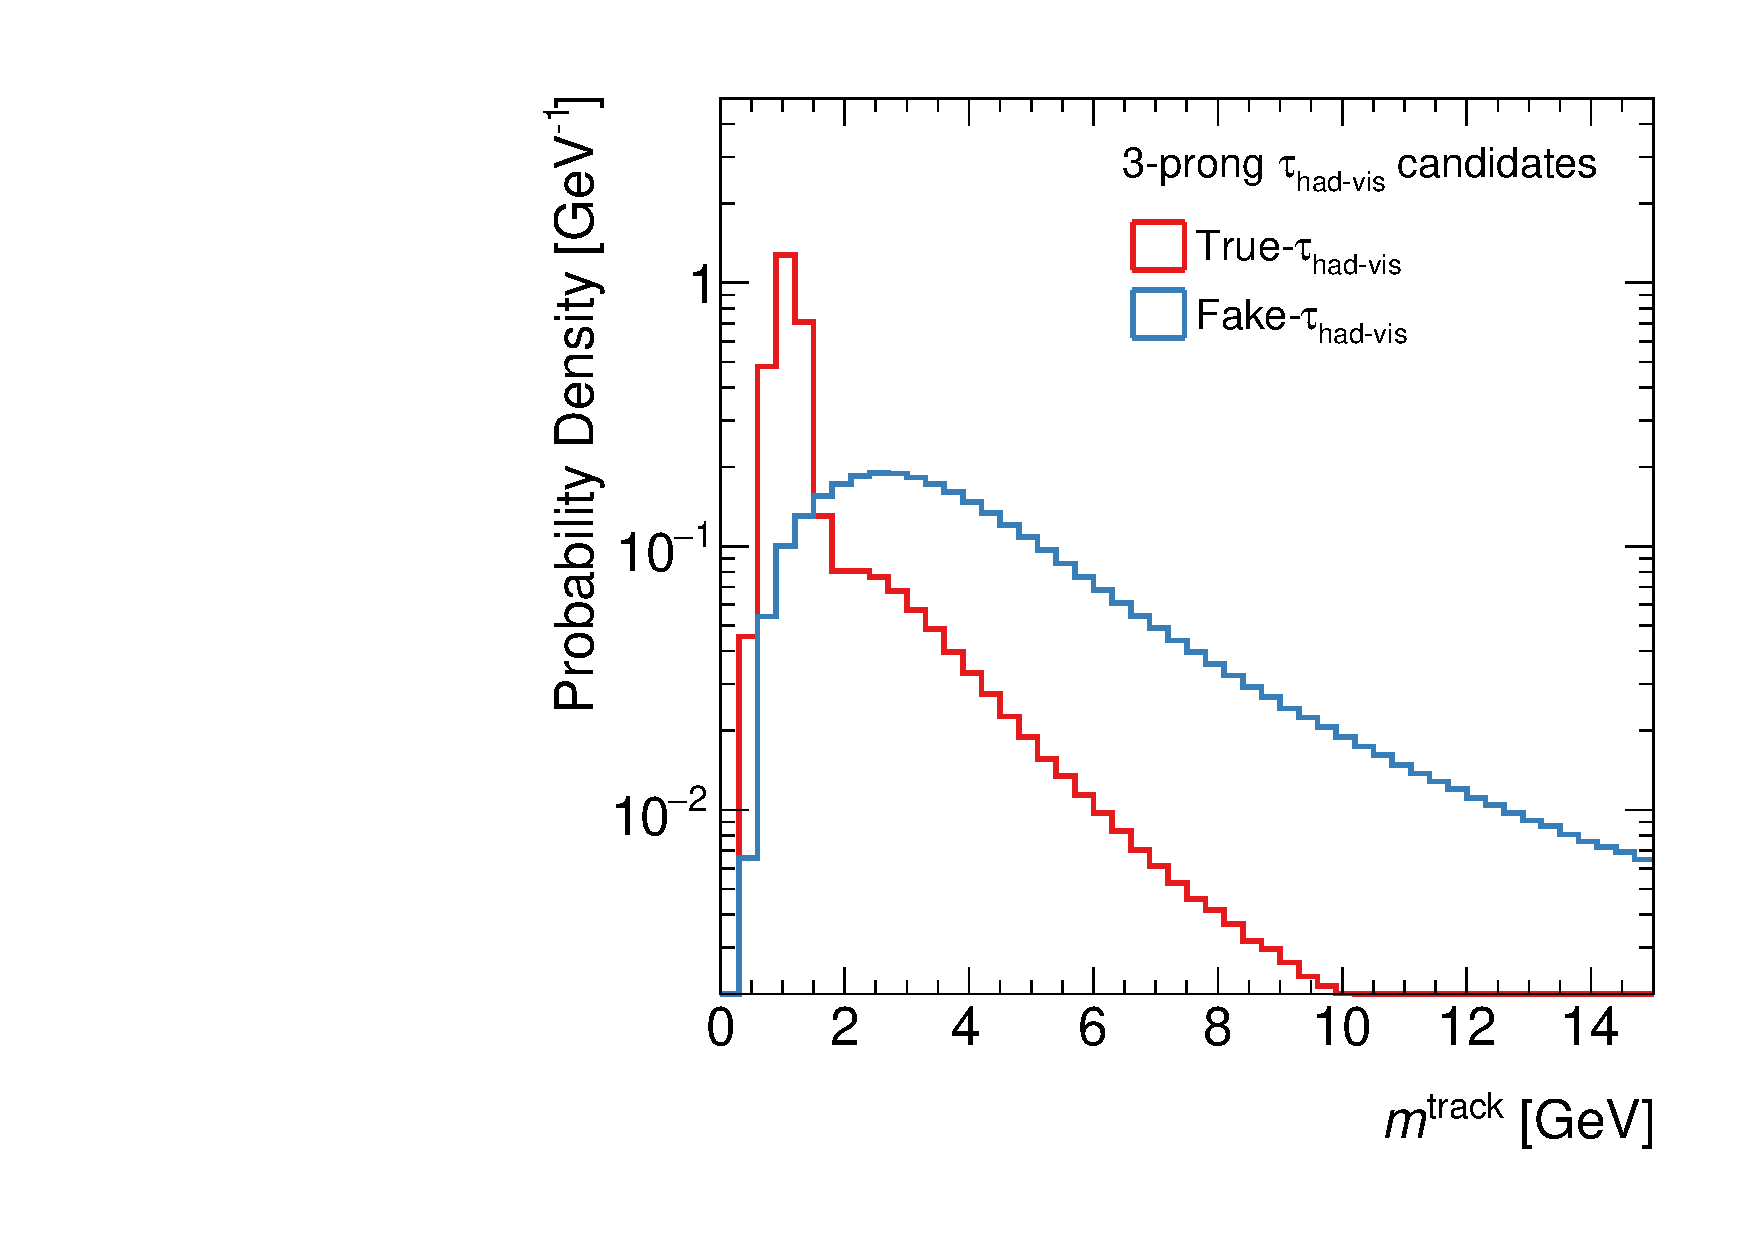
\includegraphics[width=0.9\textwidth]{tauid/invars/invars_masstrksys_3P}
%     \end{columns}

%     \vspace*{0.5em}

%     \begin{itemize}
%     \item Total 11 discriminating variables considered
%     \item Previously used in \emph{Boosted Decision Trees} (BDTs) for Tau-ID
%     \end{itemize}
%   \end{columns}
% \end{frame}

% ------------------------------------------------------------------------------

% \begin{frame}{Previous Tau Identification Approach}
%     \begin{center}
%     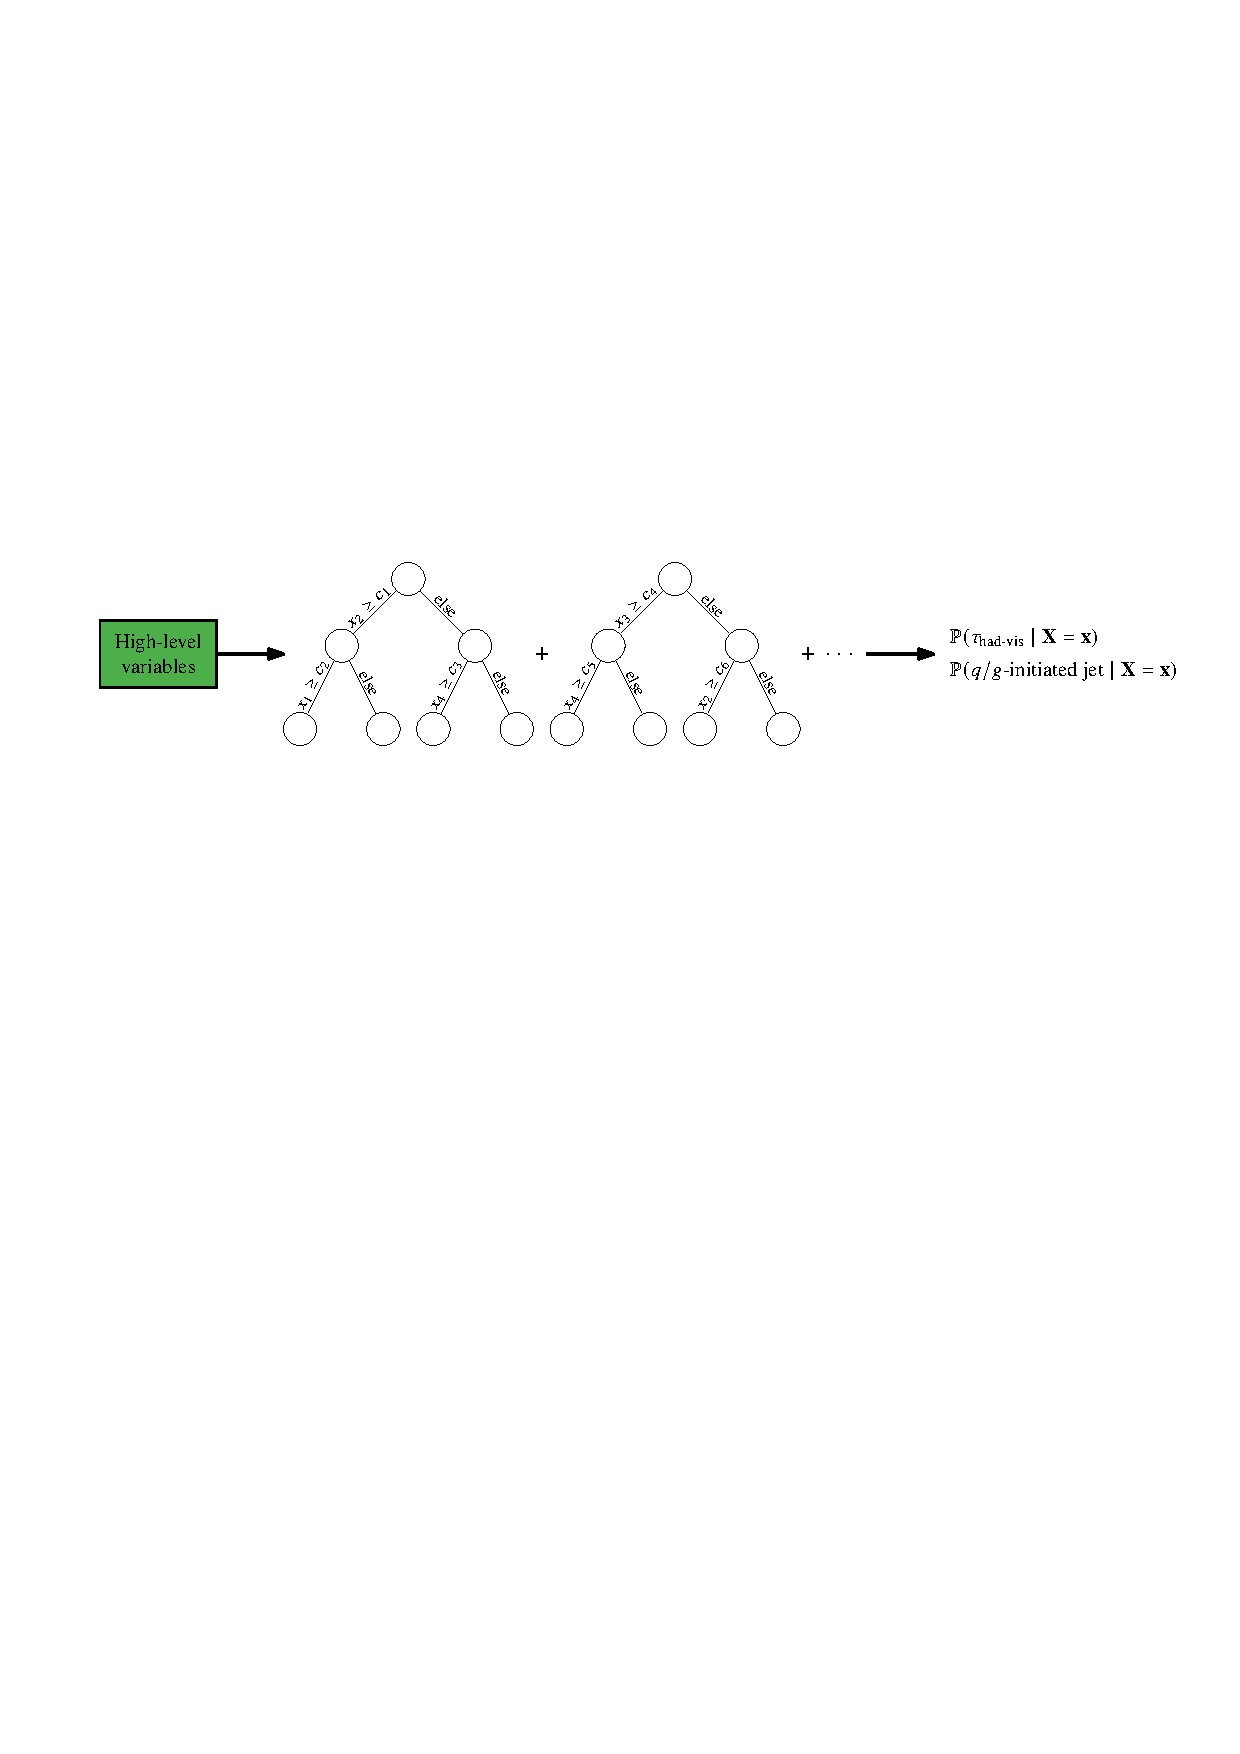
\includegraphics[scale=0.75]{tauid/bdt_approach}
%   \end{center}

%   Using Boosted Decision Trees.
% \end{frame}

% ------------------------------------------------------------------------------

% \begin{frame}{Tau Identification with RNN}
%   \begin{columns}[onlytextwidth]
%     \column{0.25\textwidth} \centering

%     
\includegraphics[scale=1]{tauid/track_icon}

%     \column{0.75\textwidth}

%     {\centering
%       $p_{\text{T}}$ of leading and sub-leading track\\[0.17em]
%     }

%     \begin{columns}[onlytextwidth]
%       \column{0.5\textwidth} \centering

%       \includegraphics<1>[width=0.9\textwidth]{tauid/invars/invars_trk0relpt_1P}

%       \column{0.5\textwidth}
%       \centering

%       \includegraphics<1>[width=0.9\textwidth]{tauid/invars/invars_trk1relpt_1P}
%     \end{columns}

%     \vspace*{0.5em}

%     \begin{itemize}
%     \item Up to 10 tracks within $\Delta R < 0.4$ of tau axis
%     \item
%     \end{itemize}
%   \end{columns}
% \end{frame}

% ------------------------------------------------------------------------------

% \begin{frame}{Tau Identification with RNN}
%   \begin{columns}[onlytextwidth]
%     \column{0.25\textwidth} \centering

%     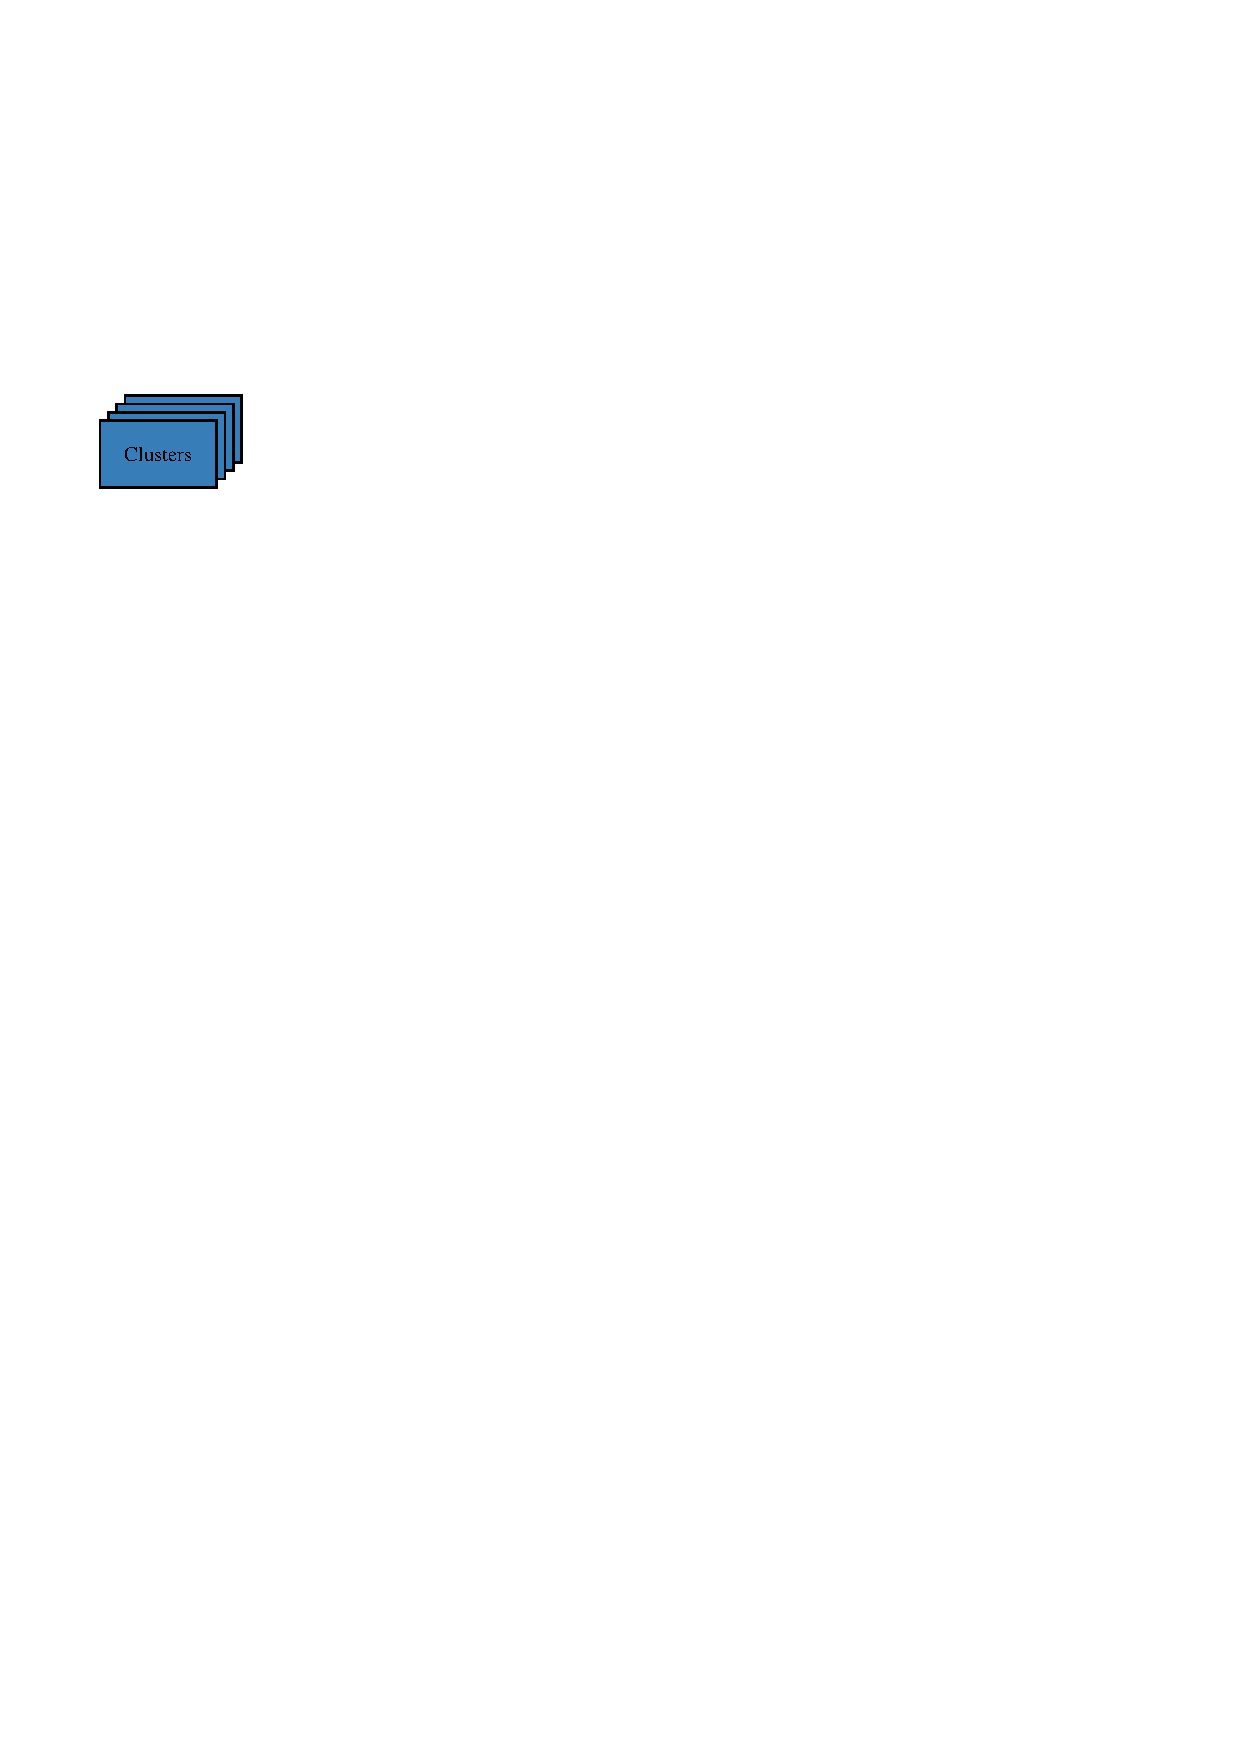
\includegraphics[scale=1]{tauid/cluster_icon}

%     \column{0.75\textwidth}

%     {\centering
%       $E_{\text{T}}$ of leading and sub-leading cluster\\[0.17em]
%     }

%     \begin{columns}[onlytextwidth]
%       \column{0.5\textwidth} \centering

%       \includegraphics<1>[width=0.9\textwidth]{tauid/invars/invars_cls0relet_3P}

%       \column{0.5\textwidth}
%       \centering

%       \includegraphics<1>[width=0.9\textwidth]{tauid/invars/invars_cls1relet_3P}
%     \end{columns}

%     \vspace*{0.5em}

%     \begin{itemize}
%     \item Up to 6 clusters associated to the jet seed
%     \item
%     \end{itemize}
%   \end{columns}
% \end{frame}

% ------------------------------------------------------------------------------

\begin{frame}{Tau Identification:\ Network Architecture}
  \begin{center}
    \begin{overpic}[width=\textwidth]{tauid/rnn_approach}
      % \put(55,35){\textbf{Lala}}

      \put(36,-1.5){%
        \parbox{3.0in}{\color{orange_cb}Recurrent neural network~(RNN)
          architecture to process sequences of tracks/clusters}%
      }
    \end{overpic}
  \end{center}
\end{frame}

% ------------------------------------------------------------------------------

% \begin{frame}{Tau Identification:\ Performance}
%   \vspace*{0.5em}
%   \begin{columns}[onlytextwidth]
%     \column{0.5\textwidth} \centering\footnotesize

%     \begin{tabular}{lcc}
%       \toprule
%       & \multicolumn{2}{c}{\textbf{Rejection Improvement}}\\
%       \textbf{Working Point} & {\hspace*{0.8em}1-prong\hspace*{0.8em}} & {\hspace*{0.8em}3-prong\hspace*{0.8em}} \\
%       \midrule
%       Very Loose (VL) & +85\,\% & +40\,\% \\
%       Loose (L)       & +75\,\% & +50\,\% \\
%       Medium (M)      & +80\,\% & +60\,\% \\
%       Tight (T)       & +80\,\% & +80\,\% \\
%       \bottomrule
%     \end{tabular}

%     \vspace*{1.75em}

%     \column{0.5\textwidth}

%     \begin{overpic}[width=1.0\textwidth]{tauid/roc_incl_witherrors}
%       \put(51,55){\footnotesize\color{blue_cb}T}
%       \put(62.3,48.5){\footnotesize\color{blue_cb}M}
%       \put(74.5,42.5){\footnotesize\color{blue_cb}L}
%       \put(88.5,33){\footnotesize\color{blue_cb}VL}

%       \put(64.5,34.2){\scriptsize\color{red_cb}T}
%       \put(73.5,25){\footnotesize\color{red_cb}M}
%       \put(82,21.8){\footnotesize\color{red_cb}L}
%       \put(88.5,16){\footnotesize\color{red_cb}VL}
%     \end{overpic}
%   \end{columns}

%   \begin{itemize}
%     \setlength{\itemsep}{0.5em}

%   \item Recommended identification algorithm for analyses of the Run~2 dataset

%   \item Adopted for tau identification in the high-level trigger (end of Run~2
%     \& Run~3)

%   \end{itemize}
% \end{frame}

\begin{frame}{Tau Identification:\ Performance Improvement}

  %\begin{columns}[onlytextwidth]
  %  \column{0.6\textwidth}

  \vspace*{1em}

  \begin{center}
    \begin{overpic}[width=0.6\textwidth]{tauid/roc_incl_witherrors}
      % \put(51,55){\footnotesize\color{blue_cb}\onslide<1>{T}}
      % \put(62.3,48.5){\footnotesize\color{blue_cb}\onslide<1>{M}}
      % \put(74.5,42.5){\footnotesize\color{blue_cb}\onslide<1>{L}}
      % \put(88.5,33){\footnotesize\color{blue_cb}\onslide<1>{VL}}

      % \put(64.5,34.2){\scriptsize\color{red_cb}\onslide<1>{T}}
      % \put(73.5,25){\footnotesize\color{red_cb}\onslide<1>{M}}
      % \put(82,21.8){\footnotesize\color{red_cb}\onslide<1>{L}}
      % \put(88.5,16){\footnotesize\color{red_cb}\onslide<1>{VL}}

      \put(19,50.5){\onslide<2->{\rotatebox{-26}{\small\color{red_cb}\textbf{80\,\% rej.\
              improvement}}}}

      \put(42,60){\onslide<2->{\rotatebox{-26}{\small\color{blue_cb}\textbf{40--80\,\% rej.\
              improvement}}}}

    \end{overpic}
  \end{center}
    %\column{0.4\textwidth}

    % \begin{itemize}
    %   \setlength{\itemsep}{1em}

    % \item<2-> Default identification algorithm for analyses of the Run~2 dataset

    % \item<2-> Adopted for use in the high-level trigger (end of Run~2 \& Run~3)

    % \end{itemize}
  % \end{columns}
\end{frame}

% ------------------------------------------------------------------------------

\begin{frame}[standout]
  Search for Higgs Boson Pair Production

  \vspace*{1.5em}

  
\includegraphics[width=0.6\textwidth]{final_state/final_state_hadhad_inverted}
\end{frame}

% ------------------------------------------------------------------------------

\begin{frame}{Event Selection}
  \begin{center}
    \begin{tabular}{c@{\hskip 2em}c@{\hskip 3em}c}
      \toprule
      \textcolor{Blue}{\hadhad} & \textcolor{lhred}{\lephad (SLT)} & \textcolor{lhred}{\lephad (LTT)} \\
      \midrule
      \textcolor{Blue}{single- \& di-\tauhadvis triggers} & \textcolor{lhred}{single-$\ell$ triggers} & \textcolor{lhred}{$\ell+\tauhadvis$ triggers} \\
      \textcolor{Blue}{exactly two $\tauhadvis$} & \multicolumn{2}{c}{\textcolor{lhred}{exactly one $\tauhadvis$}} \\
      \textcolor{Blue}{no $e$ or $\mu$} & \multicolumn{2}{c}{\textcolor{lhred}{exactly one $e$ or $\mu$}} \\
                                  %& \multicolumn{2}{c}{\textcolor{lhred}{$m_{bb} < \SI{150}{\GeV}$}} \\
      \midrule
      %\multicolumn{3}{c}{trigger-dependent \pT cuts on $e$/$\mu$/$\tauhadvis$ and jets} \\
      \multicolumn{3}{c}{$m_{\tau\tau} > \SI{60}{\GeV}$} \\
      \multicolumn{3}{c}{2 $b$-tagged jets} \\
      \multicolumn{3}{c}{OS electric charge of $e / \mu / \tauhadvis$ and \tauhadvis} \\
      \bottomrule
    \end{tabular}
  \end{center}

  \onslide<1>{
    \begin{tikzpicture}[remember picture,overlay,shift=(current page.south
      west),x=(current page.south east),y=(current page.north west)]
      \filldraw[white](0.08,0.1) rectangle (0.92,0.48);
    \end{tikzpicture}
  }
  \onslide<2>{}

  % \begin{minipage}[c]{0.45\textwidth}
  %   \centering
  %   \small

  %   Acceptance of non-res.\ $HH$ (SM):

  %   \vspace{1em}

  %   \begin{tabular}{lc}
  %     \toprule
  %     Channel & $(\mathcal{A} \times \varepsilon)^\text{ggF+VBF}_{\text{SM } HH}$ \\
  %     \midrule
  %     \hadhad & 4.0\,\% \\
  %     \lephad (SLT) & 4.0\,\% \\
  %     \lephad (LTT) & 0.97\,\% \\
  %     \bottomrule
  %   \end{tabular}
  % \end{minipage}%
  % \begin{minipage}[c]{0.55\textwidth}
  %   \centering
  %   \small

  %   %Acceptance of narrow scalar resonances:

  %   %\vspace{0.4em}

  %   \begin{overpic}[width=0.9\textwidth]{selection/acceptance_resonant}
  %     %\put(54.5,68){\scriptsize ATLAS-CONF-2021-030}
  %   \end{overpic}
  % \end{minipage}

  % \onslide<2->{
  %   \tikz[overlay, remember picture,
  %   shift=(current page.south west),
  %   x=(current page.south east), y=(current page.north west),
  %   ]{
  %     \node[align=center]at (0.5,0.678) {
  %       \setlength{\fboxrule}{1pt}
  %       \fcolorbox{headergray}{mygray}{%
  %         \begin{minipage}{0.75\textwidth}
  %           \vspace*{0.6em}
  %           \begin{itemize}
  %             \setlength{\itemsep}{1em}
  %           \item Close to \alert{two-fold improvement in signal acceptance} compared to previous publication\\
  %             {\scriptsize (Phys. Rev. Lett. \textbf{121}, 191801)}

  %           \item Driven by \alert{improved reconstruction and identification
  %             of $\tauhad$ and $b$-jets}\\
  %             {\scriptsize (ATL-PHYS-PUB-2017-003, ATL-PHYS-PUB-2017-013, ATL-PHYS-PUB-2019-033)}

  %           \end{itemize}
  %           \vspace*{0.8em}
  %         \end{minipage}
  %       }
  %     };
  %     % Optional help grid lines
  %     % \draw[step=.1, opacity=0.3, thick, red] (0,0) grid (1,1);
  % } }
\end{frame}

% ------------------------------------------------------------------------------


% ------------------------------------------------------------------------------

% \begin{frame}{Signal Acceptance Improvement}
%   \begin{center}
%     \begin{tabular}{l@{\hskip 2em}c@{\hskip 2em}c}
%       \toprule
%       & \allbold{This Analysis} & Previously \\
%       \cmidrule{2-3}
%       Channel & $(\mathcal{A} \times \varepsilon)^{gg\text{F+VBF}}_{\text{SM } HH}$ & $(\mathcal{A} \times \varepsilon)^{gg\text{F}}_{\text{SM } HH}$ \\
%       \midrule
%       \hadhad & 4.0\,\%\phantom{7} & 1.9\,\% \\
%       \lephad (SLT) & 4.0\,\%\phantom{7} & \multirow{2}{*}{\hspace*{-1.05em}\bigg\} 3.2\,\%}\\
%       \lephad (LTT) & 0.97\,\% & \\
%       \bottomrule
%     \end{tabular}
%   \end{center}

%   \vspace*{1em}

%   \alert{Signal acceptance improvement of \SIrange{50}{100}{\percent}} compared
%   to previous publication {\scriptsize (Phys.~Rev.~Lett.~\textbf{121},~191801)}
% \end{frame}

% ------------------------------------------------------------------------------

% \begin{frame}{Background Estimation: Overview}
%     \begin{minipage}{0.5\textwidth}
%     \centering

%     \begin{overpic}[width=0.65\textwidth]{mhh_hadhad}
%       \put(56,94){\tiny arXiv:2209.10910}
%     \end{overpic}
%   \end{minipage}%
%   \begin{minipage}{0.5\textwidth}
%     \centering

%     \begin{overpic}[width=0.65\textwidth]{mhh_lephad}
%       \put(56,94){\tiny arXiv:2209.10910}
%     \end{overpic}
%   \end{minipage}

%   \centering

%   \resizebox{0.8\textwidth}{!}{%
%     \begin{tabular}{lcc}
%       \toprule
%       Background & \hadhad channel & \lephad channel \\
%       \midrule
%       \ttbar & \multicolumn{2}{c}{\textcolor{toporange}{Simulation (normalised in fit)}} \\[0.1em]
%       Z+jets & \multicolumn{2}{c}{\allbold{\textcolor{zjetsgreen}{Simulation (normalised in fit -- dedicated CR)}}} \\[0.1em]
%       Jet \ra fake-\tauhadvis (\ttbar) & \allbold{\textcolor{topfakered}{Simulation + scale factors}} & \multirow{2}{*}{\textcolor{fakeblue}{Combined fake factor method}} \\[0.1em]
%       Jet \ra fake-\tauhadvis (multi-jet) & \allbold{\textcolor{fakeblue}{Fake factor method}} & \\[0.1em]
%       Single Higgs boson / Other & \multicolumn{2}{c}{Simulation} \\[0.1em]
%       \bottomrule
%     \end{tabular}
%   }

%   % Dominant backgrounds:
%   % Z+jets: 18\,\%
%   % Top quark: 39\,\%
%   % fakes (ttbar + multijet): 40\,\%

%   % Dominant backgrounds:
%   % ttbar: 62\,\%
%   % Fakes: 34\,\%
%   % Z+jets: 2\,\%
% \end{frame}



% ------------------------------------------------------------------------------

\begin{frame}{Anatomy of High-Energy Physics Plots}
  \begin{tikzpicture}[remember picture,overlay,shift=(current page.south
      west),x=(current page.south east),y=(current page.north west)]

      \node (plot) at (0.5, 0.45) {%
        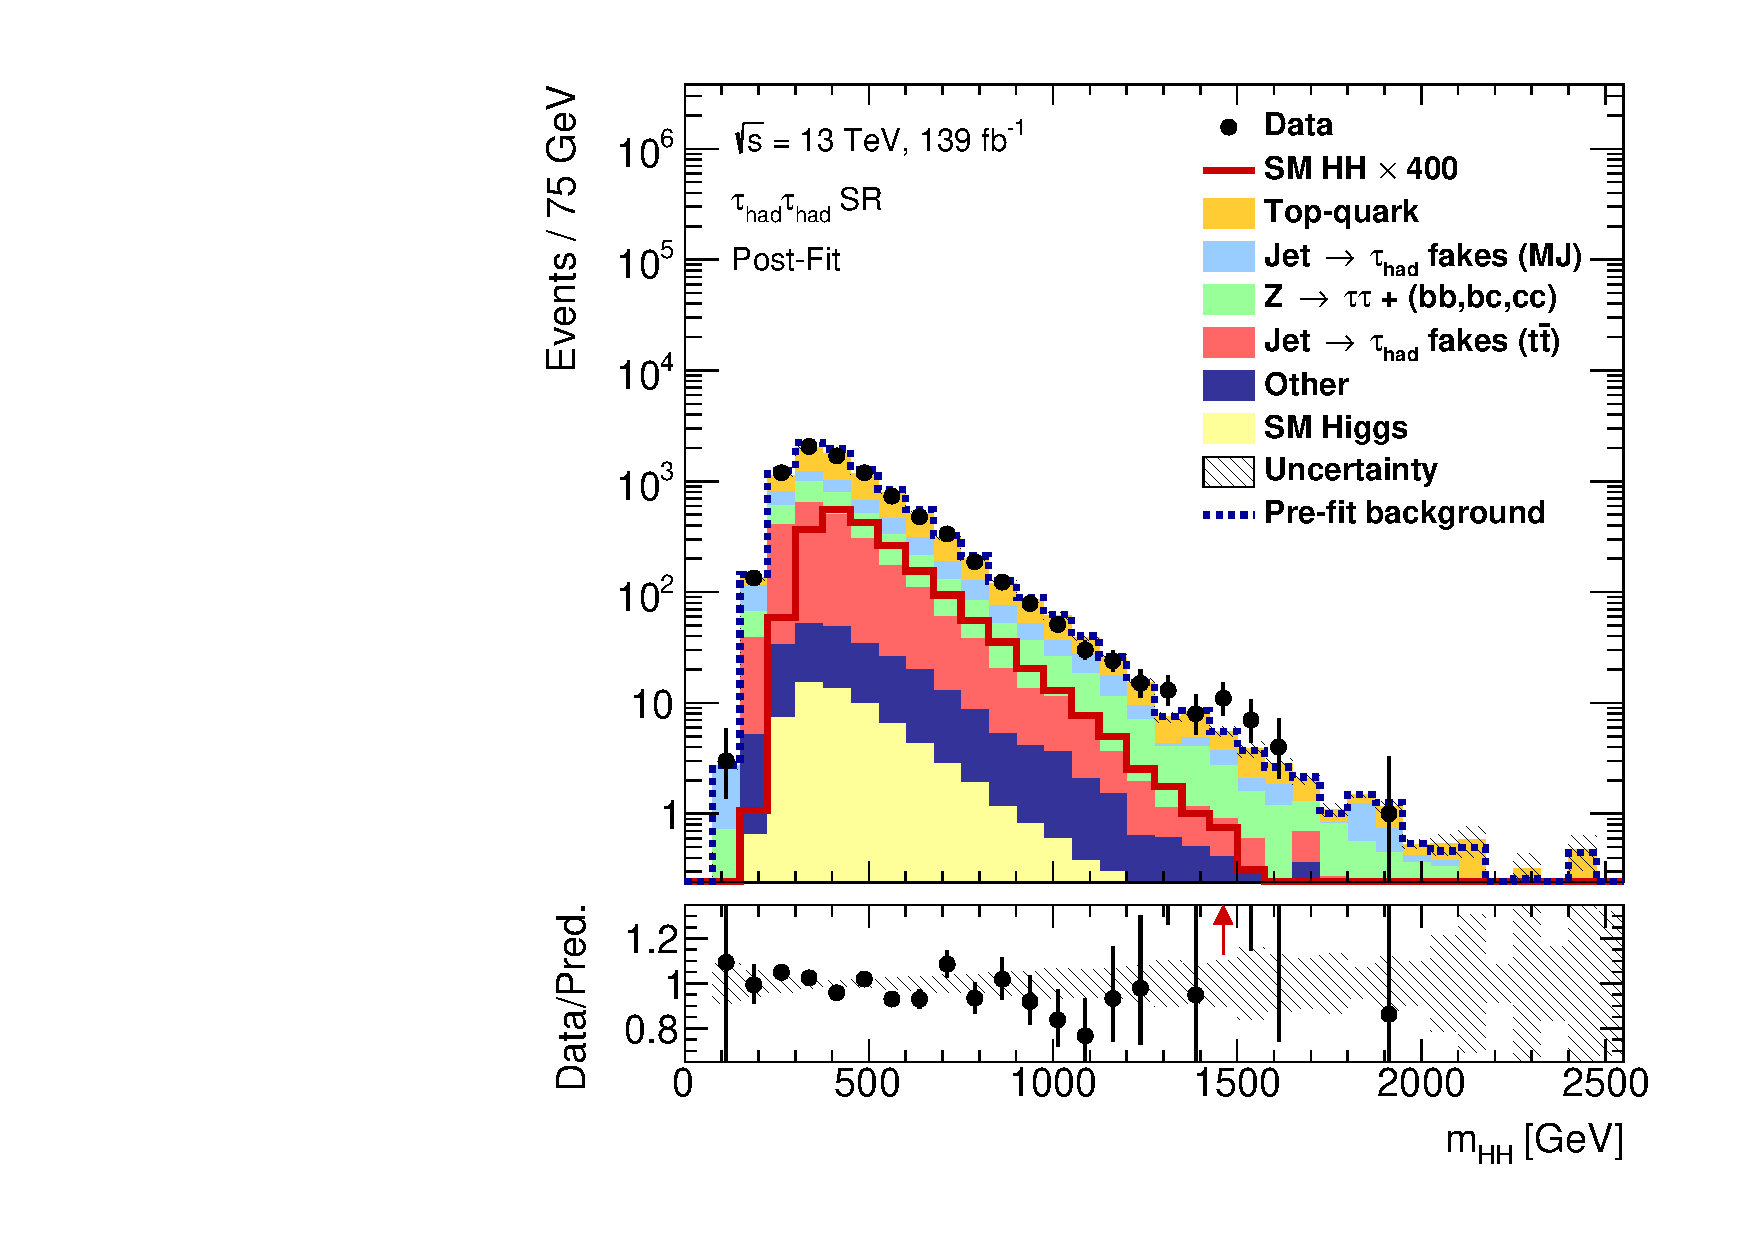
\includegraphics[width=0.5\textwidth]{results_nonres/postfit_mvainputs/Region_BMin0_incJet1_distmHH_J2_Y2015_DLLOS_T2_SpcTauHH_L0_GlobalFit_conditionnal_mu0log}%
      };

      \node at (0.515, 0.85) {\allbold{SR of the \hadhad Channel}};

      \onslide<2->{%
        \draw[stealth-, line width=2pt, color=Black] (0.555, 0.38) -- (0.75, 0.5)%
        node[right]{\allbold{Observed Data}};

        \draw[stealth-, line width=2pt, color=Black] (0.4, 0.445) -- (0.29,
        0.445)%
        node[left, align=center]{\allbold{Estimated Backgrounds}};

        \draw[stealth-, line width=2pt, color=Red] (0.53, 0.32) -- (0.75, 0.32)%
        node[right, align=center]{\allbold{SM \HH Signal}\\[-0.25ex](overlaid \& scaled)};

      %   \draw[stealth-, line width=2pt, color=Black] (0.265, 0.185) -- (0.21,
      %   0.185)%
      %   node[left, align=center]{
      %     \allbold{Ratio of Data \&}\\[-0.25ex]
      %     \allbold{$B$-only Prediction}};
      }
  \end{tikzpicture}
\end{frame}

% ------------------------------------------------------------------------------

\begin{frame}{Backgrounds in the \hadhad Channel}
  \begin{tikzpicture}[remember picture,overlay,shift=(current page.south
    west),x=(current page.south east),y=(current page.north west)]

    \node (plot) at (0.5, 0.45) {%
      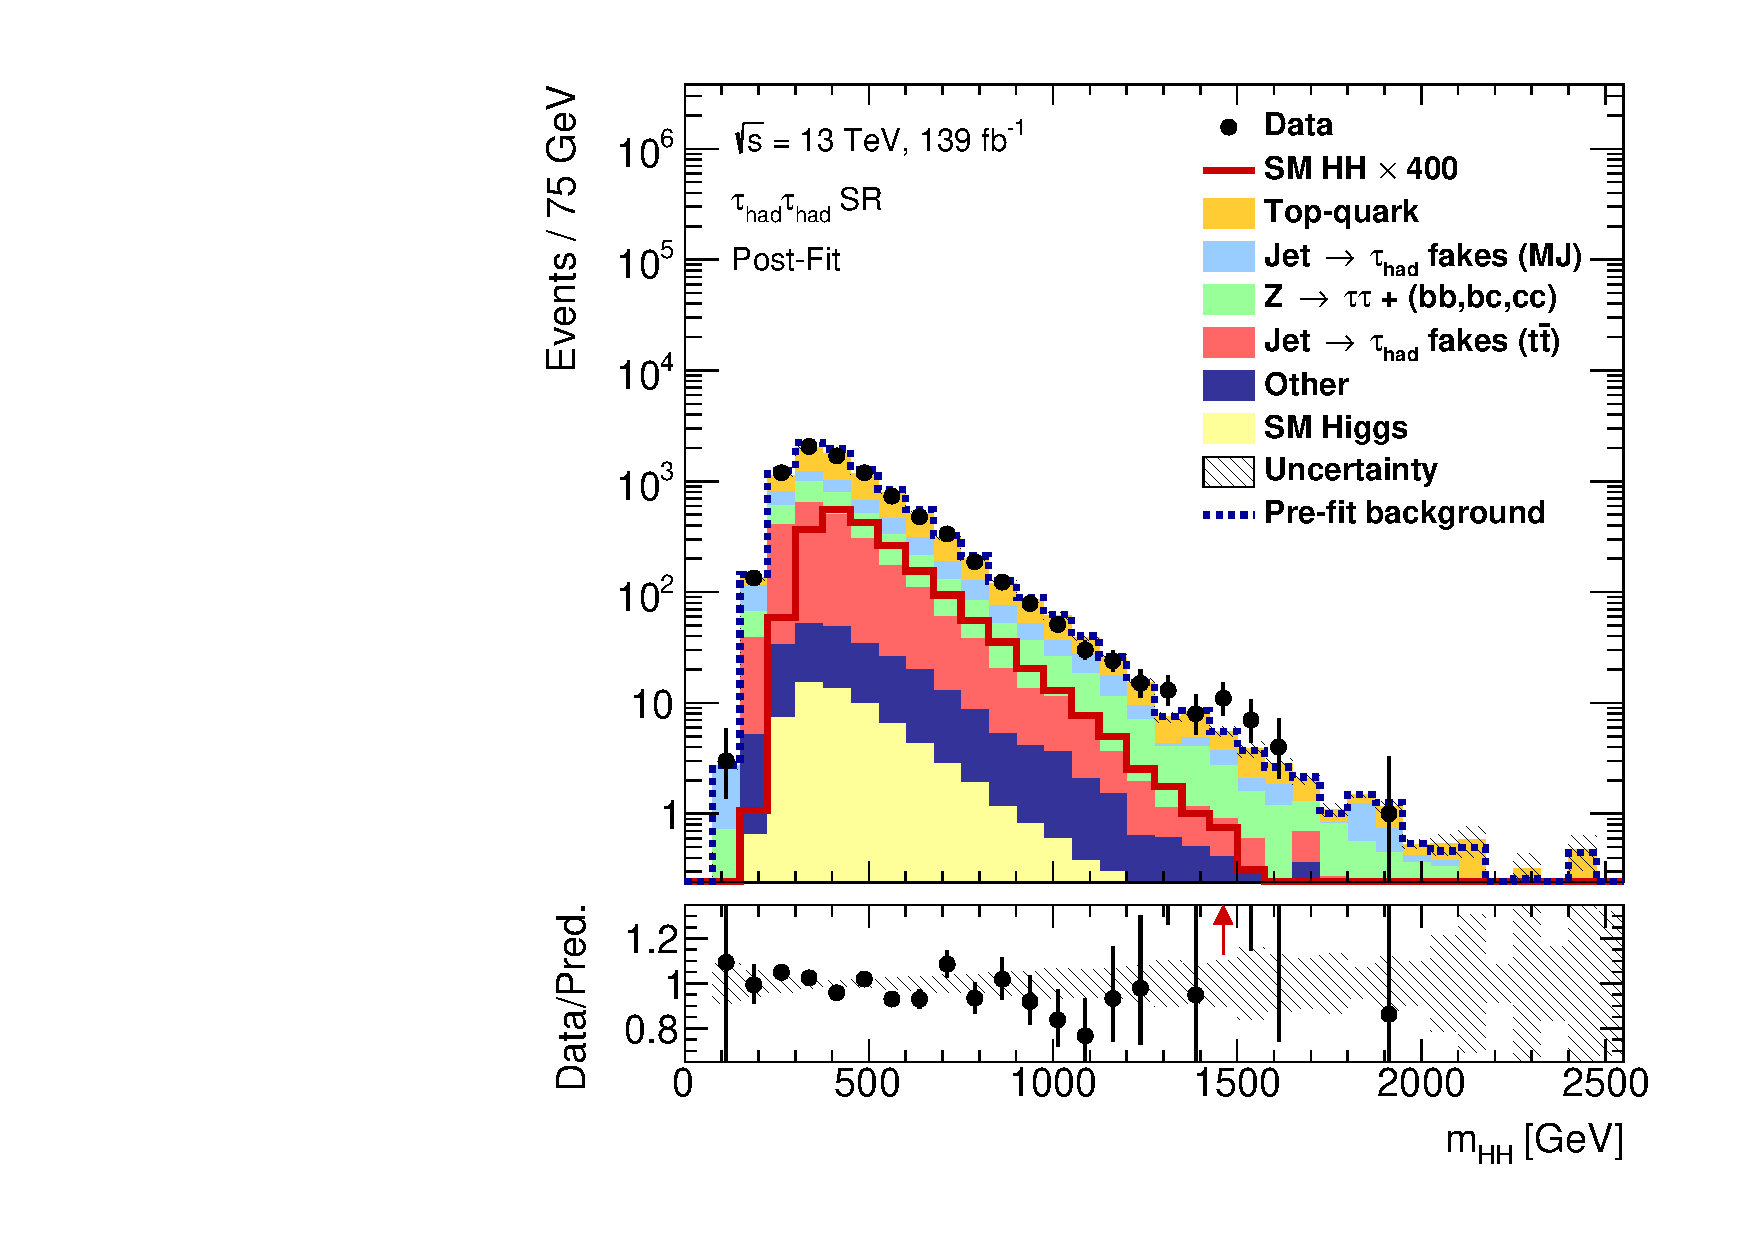
\includegraphics[width=0.5\textwidth]{results_nonres/postfit_mvainputs/Region_BMin0_incJet1_distmHH_J2_Y2015_DLLOS_T2_SpcTauHH_L0_GlobalFit_conditionnal_mu0log}%
    };

    \node at (0.515, 0.85) {\allbold{SR of the \hadhad Channel}};

    \onslide<1>{%
      \draw[stealth-, line width=2pt, color=Black] (0.4, 0.445) -- (0.29,
      0.445)%
      node[left, align=center]{\allbold{Estimated Backgrounds}};
    }

    % ------------------------------------------------------------------
    % REAL TAU BACKGROUNDS
    % ------------------------------------------------------------------
    \onslide<2->{%
      \node[align=left] at (0.855, 0.65) {\allbold{Bkg.\ with real \tauhadvis}};

      \draw[stealth-, line width=2pt, color=toporange] (0.53, 0.38) -- (0.745, 0.5)%
      node[right, align=center]{\allbold{\ttbar with true \tauhadvis}\\[-0.25ex](\SI{39}{\percent})};

      \draw[stealth-, line width=2pt, color=zjetsgreen] (0.54, 0.32) -- (0.805, 0.32)%
      node[right, align=center]{\allbold{$Z$ + jets}\\[-0.25ex](\SI{18}{\percent})};
    }

    % ------------------------------------------------------------------
    % FAKE TAU BACKGROUNDS
    % ------------------------------------------------------------------
    \onslide<3->{%
      \node[align=left] at (0.15, 0.55) {\allbold{Bkg.\ with mis-id.\ \tauhadvis}};

      \draw[stealth-, line width=2pt, color=topfakered] (0.35, 0.41) -- (0.26,
      0.41)%
      node[left, align=center]{\allbold{\ttbar with fake \tauhadvis}\\[-0.25ex](\SI{25}{\percent})};

      \draw[stealth-, line width=2pt, color=fakeblue] (0.335, 0.31) -- (0.205,
      0.24)%
      node[left, align=center]{\allbold{Multi-jet}\\[-0.25ex](\SI{15}{\percent})};
    }

    \onslide<4->{%
      \filldraw[white,opacity=0.7](0.0,0.063) rectangle (1.0,0.88);

      \node[align=center] at (0.512,0.7){%
        \setlength{\fboxrule}{1pt}
        \fcolorbox{headergray}{white}{%
          \begin{minipage}[c]{0.45\textwidth}
            \vspace*{0.25em}

            \begin{tabular}{lS[table-format=4.2(3)]}
              \textbf{Exp.\ Signal:} & 5.16 +- 0.84 \\
              \textbf{Exp.\ Background:} & 8414 +- 90
            \end{tabular}

            \vspace*{1em}

            % \hspace*{0.6em}$S / \sqrt{B} = 0.06$ \ra \alert{little signal sensitivity}
            \hspace*{0.6em} \ra \alert{little signal sensitivity}

            \vspace*{0.25em}
          \end{minipage}
        }
      };
    }
  \end{tikzpicture}
\end{frame}

% ------------------------------------------------------------------------------

% What to mention:
% - H masses most important for SM HH (resolution below 18 GeV)
% - mHH most important for resonant search for intermediate to high masses (resolution 10%)

% ------------------------------------------------------------------------------

\begin{frame}{Signal Extraction}
  \begin{columns}[onlytextwidth]
    \column{0.5\textwidth}

    \textbf{Signal/background classification using machine learning:}
    \begin{itemize}
    \item Boosted decision trees (\hadhad)
    \item Neural networks (\lephad)
    \end{itemize}

    \vspace*{2em}

    \textbf{Classification scores are used for statistical interpretation.}

    % Most relevant backgrounds at high score:\\
    % Z+jets (36\,\%), Fake-\tauhadvis (21\,\%), Single Higgs boson (19\,\%),
    % Top-quark (17\,\%)

    \column{0.5\textwidth}
    \centering

    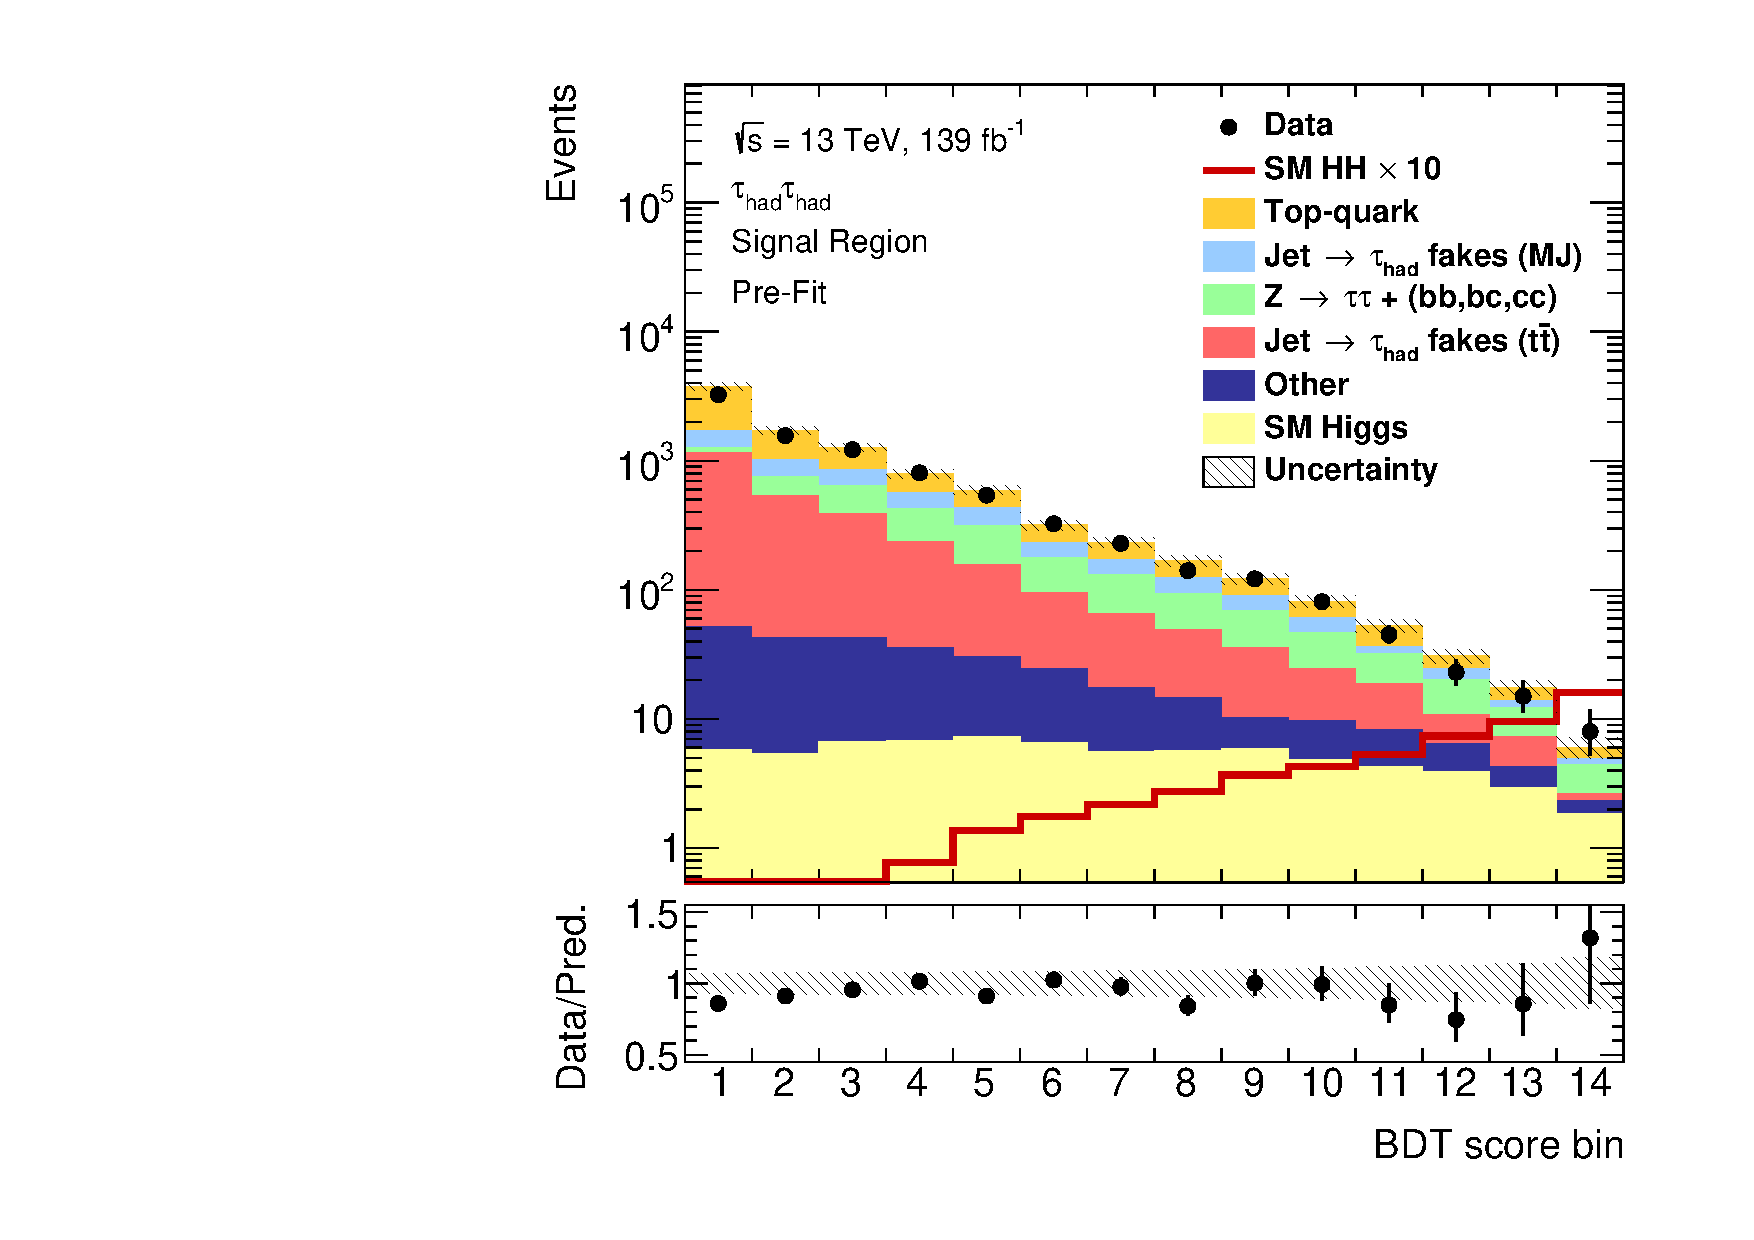
\includegraphics[width=0.9\textwidth]{mva/prefit/Region_BMin0_incJet1_distSMBDT_J2_Y2015_DLLOS_T2_SpcTauHH_L0_Prefitlog}
  \end{columns}
  \tikz[overlay, remember picture, shift=(current page.south west), x=(current
  page.south east), y=(current page.north west), ]{%
    \draw[stealth-, line width=1.5pt, color=Blue] (0.58,0.13) -- (0.735,0.13);
    \node at (0.6575, 0.13 - 0.03) {\footnotesize \color{Blue} background-like};
    \draw[-stealth, line width=1.5pt, color=Red] (0.755,0.13) -- (0.91,0.13);
    \node at (0.8325, 0.13 - 0.03) {\footnotesize \color{Red} signal-like};
  }
\end{frame}



% Verbally mention some features:
% - Only one NN needed for a continuously varying classification task
% - Ability to interpolate
% - Up to 20% improvement in signal sensitivity compared to previous approach

% ------------------------------------------------------------------------------

% \begin{frame}{Statistical Analysis}
%   \begin{center}
%     \begin{tabular}{l@{\hskip 1em}cccc}
%       \toprule
%       &\multicolumn{4}{c}{\textbf{Discriminant used in channel}} \\
%       \cmidrule{2-5}
%       \textbf{Search} & \hadhad & \lephad SLT & \lephad LTT & $Z+\text{HF}$ CR \\
%       \midrule
%       SM~\HH Production & {\color{red_cb}BDT} & {\color{purple_cb}NN} & {\color{purple_cb}NN} & {\color{green_cb}$m_{\ell\ell}$} \\
%       Resonant \HH Production & {\color{blue_cb}$\text{PNN}(m_{X})$} & {\color{blue_cb}$\text{PNN}(m_{X})$} & {\color{blue_cb}$\text{PNN}(m_{X})$} & {\color{green_cb}$m_{\ell\ell}$} \\
%       \bottomrule
%     \end{tabular}
%   \end{center}

%   % \vspace*{1em}

%   % {\footnotesize
%   %   \textbf{Statistical Model:}\\[0.5em]
%   %   \begin{itemize}
%   %     \setlength{\itemsep}{0.5em}

%   %   \item Models the binned distributions of discriminants in all channels

%   %   \item Processes with free normalisation: signal, \ttbar, $Z+\text{HF}$

%   %     % \item Additional d.o.f.\ to account for experimental \& theory uncertainties
%   %   \item Additional d.o.f.\ to account for uncertainties

%   %   \end{itemize}
%   % }
% \end{frame}

% ------------------------------------------------------------------------------

\begin{frame}[standout]
  Results of the SM~\allbold{\HH} Search

  \vspace*{1.5em}

  
\includegraphics[scale=1.0]{feynman_graphs/di_higgs_box_inverted}%
  \hspace*{2em}%
  \raisebox{0.32em}{
\includegraphics[scale=1.0]{feynman_graphs/di_higgs_triangle_inverted}}
\end{frame}



% ------------------------------------------------------------------------------

\begin{frame}{Results of the SM \allbold{\HH} Search}
  \vspace*{0.5em}
  \begin{columns}
    \column{0.333\textwidth}
    \centering

    \allbold{\hadhad channel}

    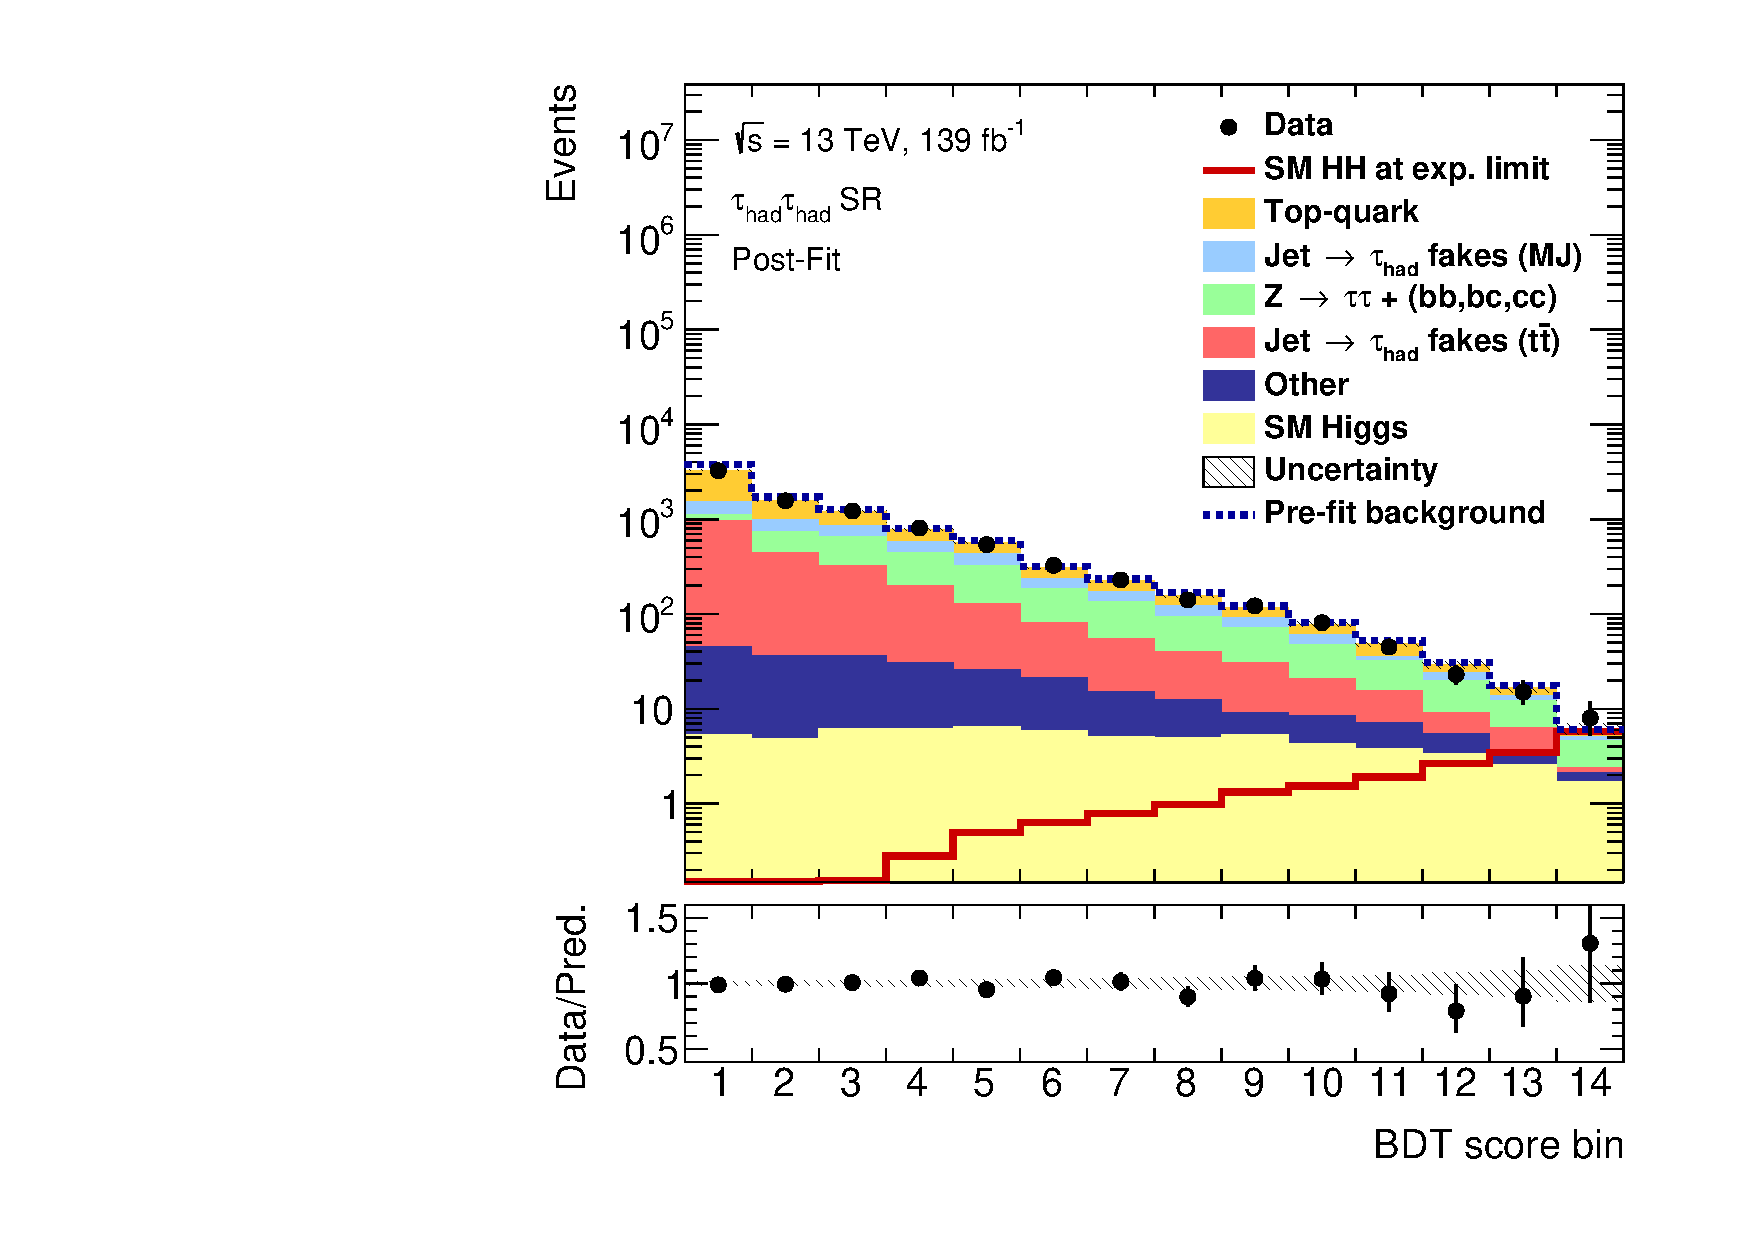
\includegraphics[width=\textwidth, trim=0.5em 0 2.5em 0, clip]{results_nonres/postfit/Region_BMin0_incJet1_distSMBDT_J2_Y2015_DLLOS_T2_SpcTauHH_L0_GlobalFit_conditionnal_mu0log}

    \column{0.333\textwidth}
    \centering

    \allbold{\lephad SLT channel}

    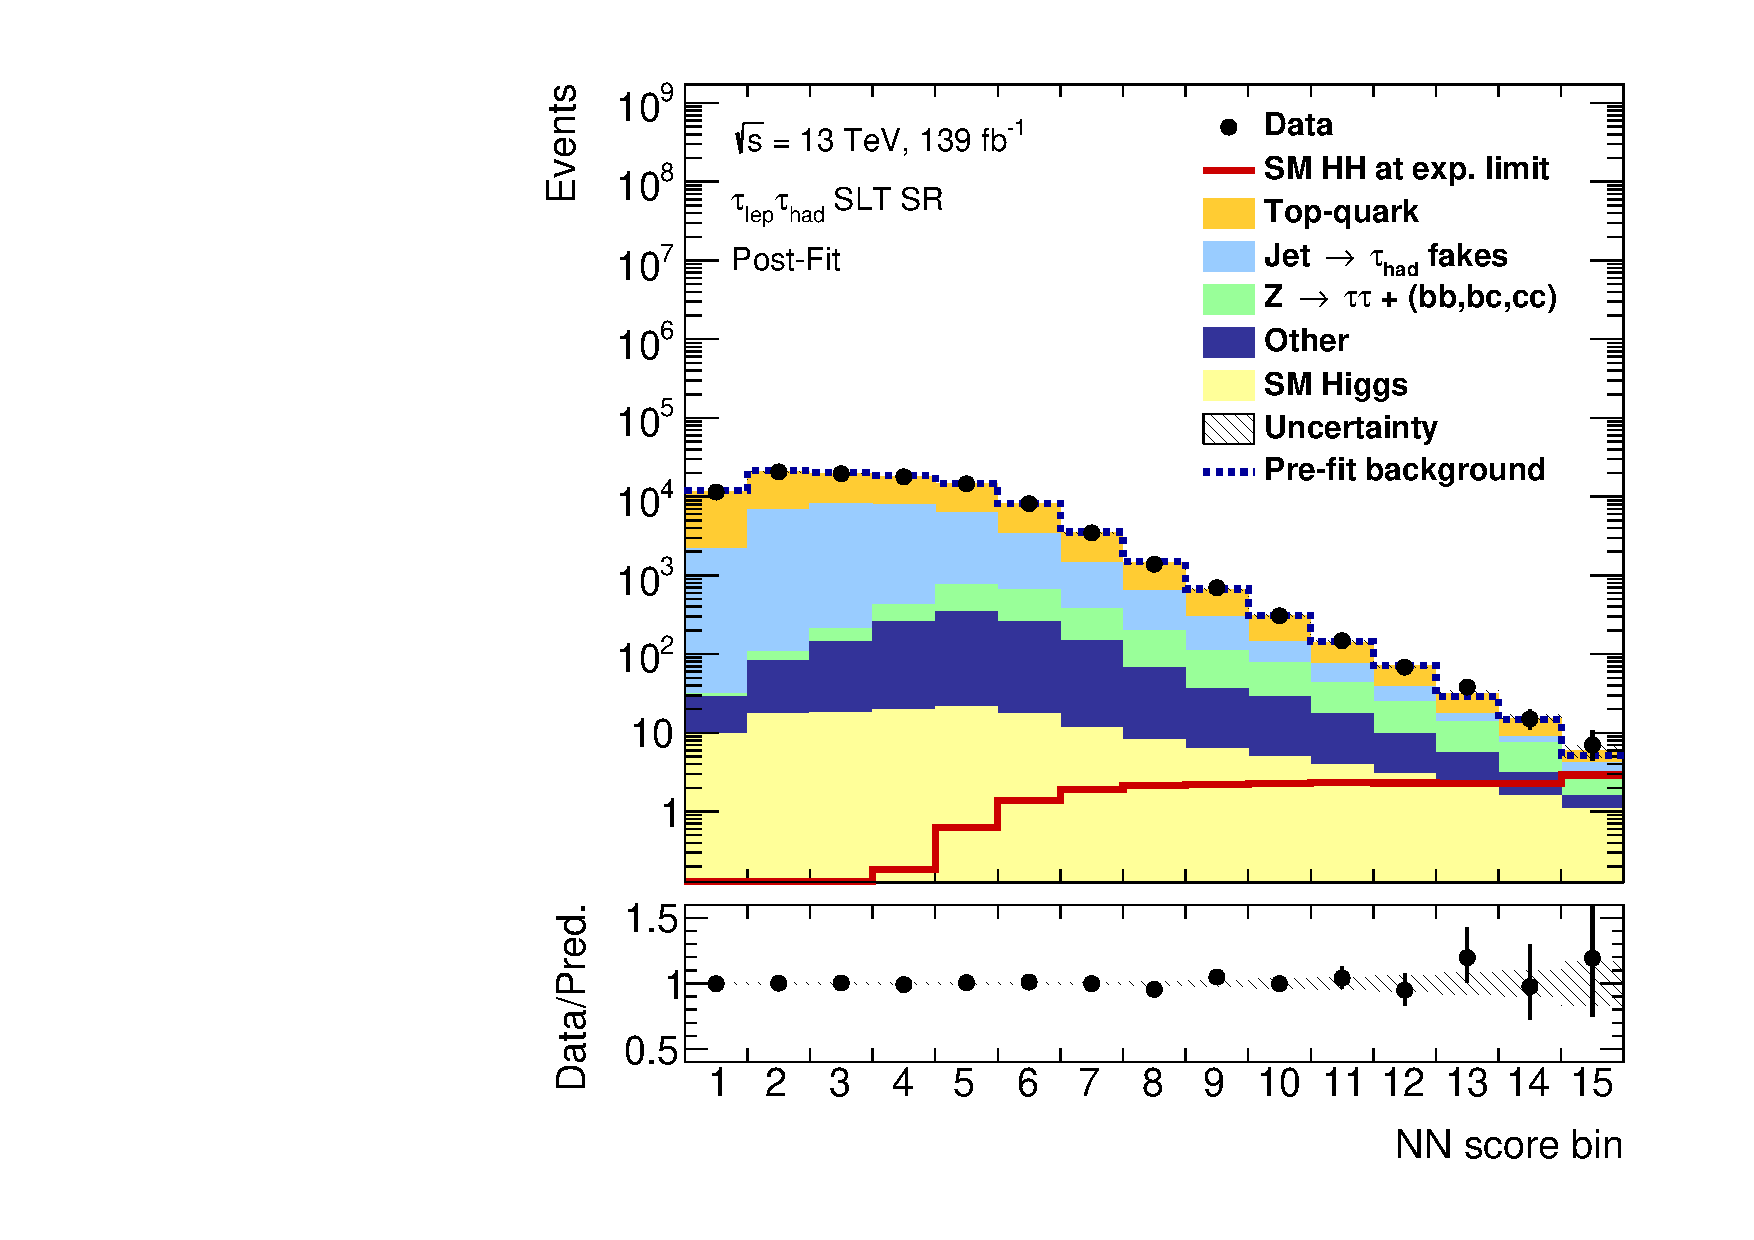
\includegraphics[width=\textwidth, trim=0.5em 0 2.5em 0, clip]{results_nonres/postfit/Region_BMin0_incJet1_distNN_J2_DSM_T2_SpcTauLH_Y2015_LTT0_L1_GlobalFit_conditionnal_mu0log}

    \column{0.333\textwidth}
    \centering

    \allbold{\lephad LTT channel}

    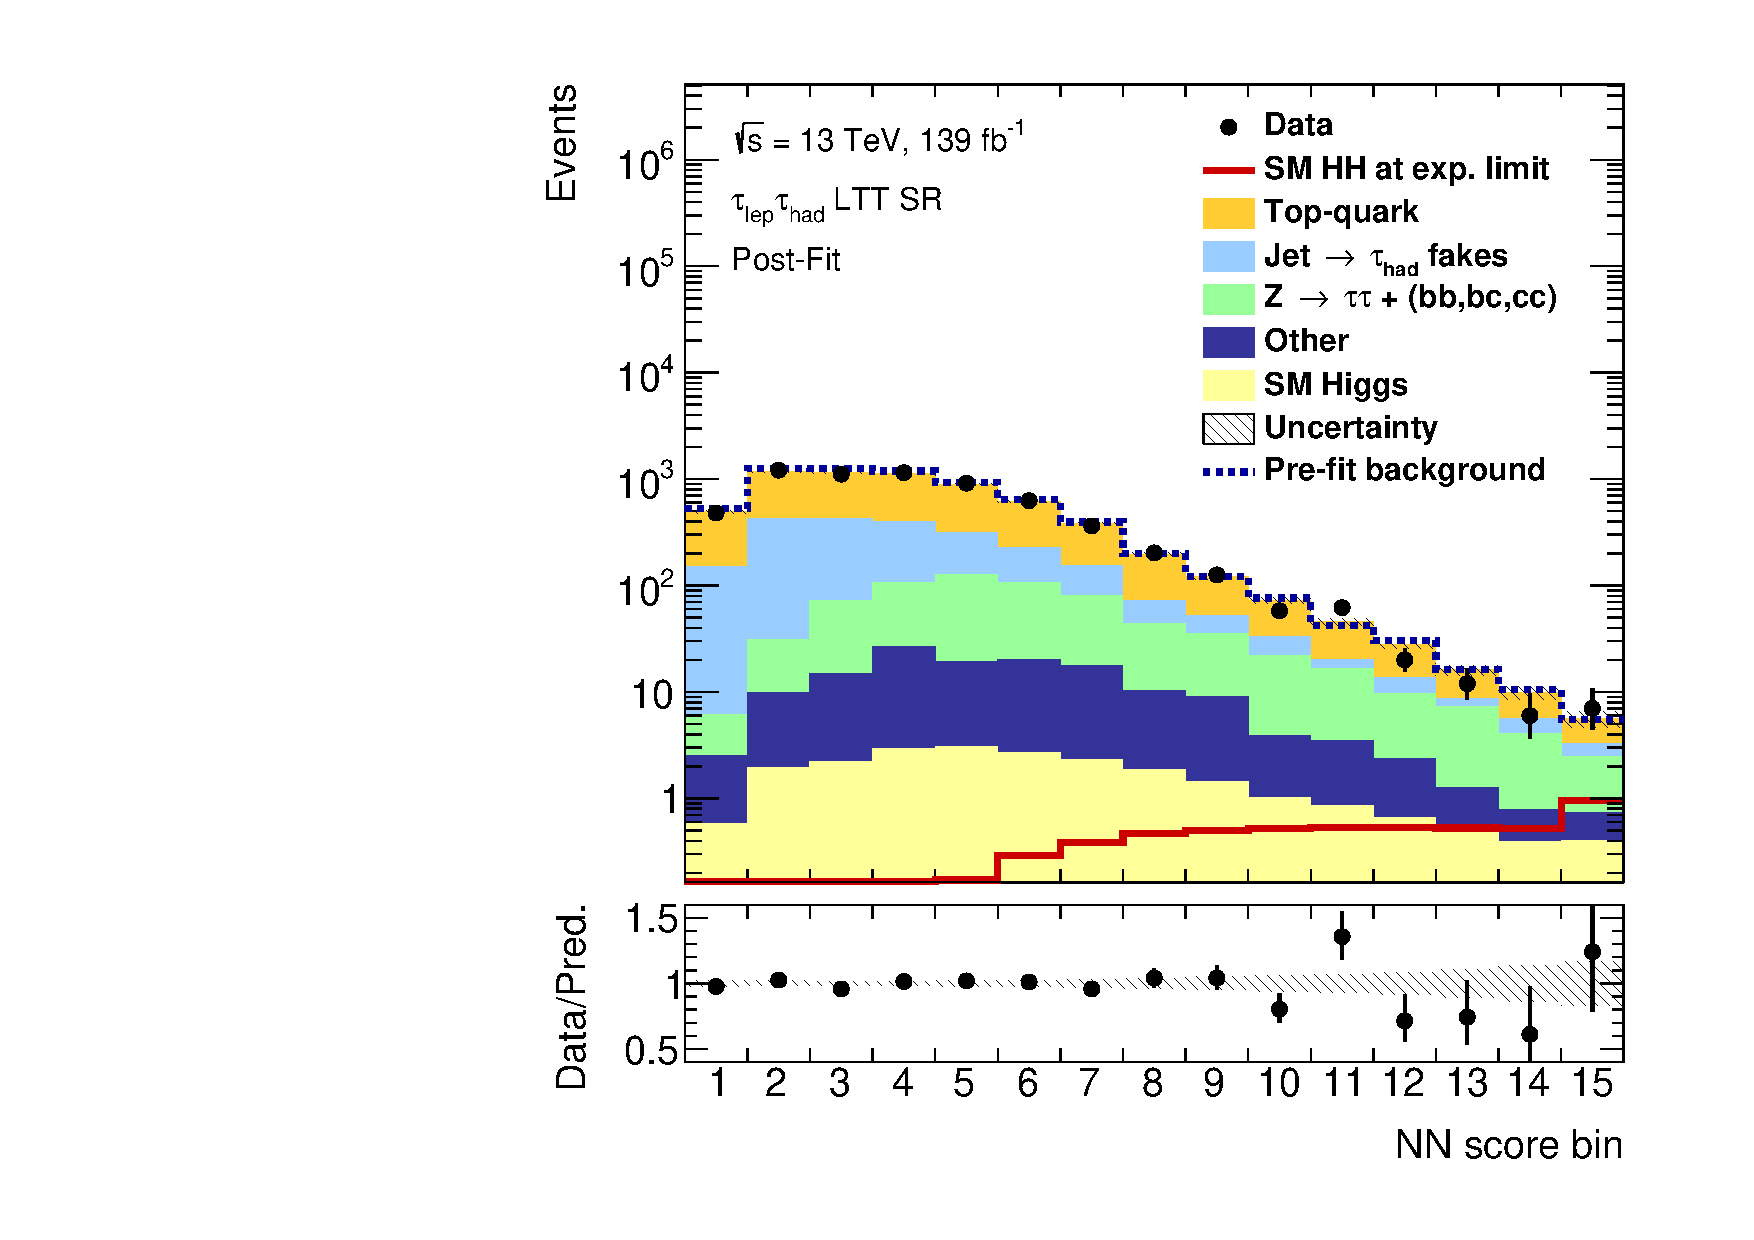
\includegraphics[width=\textwidth, trim=0.5em 0 2.5em 0, clip]{results_nonres/postfit/Region_BMin0_incJet1_distNN_J2_DSM_T2_SpcTauLH_Y2015_LTT1_L1_GlobalFit_conditionnal_mu0log}
  \end{columns}

  \vspace*{0.5em}

  \begin{itemize}
    \setlength{\itemsep}{0.75em}

  \item Agreement between background-only model and data
    ($p_0 = \SI{27}{\percent}$)

  \item Fit of signal+background model: $\hat{\mu} = 0.9^{+1.8}_{-1.5}$

  \end{itemize}
\end{frame}

% ------------------------------------------------------------------------------

\begin{frame}{Upper Limits on the SM~\boldmath{$HH$} Signal Strength}
  \vspace*{0.25em}
  \begin{center}
    \only<1>{%
      \begin{overpic}[width=0.5\textwidth]{discussion/results_139ifb_onlybbtautau}
        \put(68,85){\footnotesize arXiv:2211.01216}
      \end{overpic}
    }%
    \only<2->{%
      \begin{overpic}[width=0.5\textwidth]{discussion/results_139ifb}
        \put(68,85){\footnotesize arXiv:2211.01216}
      \end{overpic}
    }
  \end{center}

  \vspace*{-0.25em}

  \onslide<2>{\allbold{Most sensitive channel to SM~$HH$ production to date!}}

  \begin{tikzpicture}[remember picture,overlay,shift=(current page.south
    west),x=(current page.south east),y=(current page.north west)]
    \onslide<2>{%
      \draw[stealth-, line width=1pt, color=Black] (0.72, 0.5) -- (0.78, 0.5)%
      node[align=center, right]{%
        \scriptsize \bbyy re-analysis:\\[-0.4ex]
        \scriptsize 4.0 (obs.), 5.0 (exp.)\\[-0.4ex]
        \scriptsize arXiv:2310.12301
      };
    }
  \end{tikzpicture}
\end{frame}

% ------------------------------------------------------------------------------

% \begin{frame}[standout]
%   Beyond the Standard Model
% \end{frame}

% ------------------------------------------------------------------------------

% \begin{frame}{Beyond the Standard Model}
%   \begin{columns}[onlytextwidth]
%     \column{0.5\textwidth}

%     \textbf{Shortcomings of the SM:}
%     \begin{itemize}
%     \item Dark Matter \& Dark Energy
%     \item Gravitation
%     \item \dots
%     \end{itemize}

%     \column{0.5\textwidth}

%     \vspace*{0.1em}

%     \hspace*{0.35\textwidth}%
%     \begin{overpic}[scale=1,trim=0 0.3cm 0 0, clip]{energy_content/content}
%       \put(-70,37){\parbox{1.05in}{\small Energy density of the universe:}}
%       \put(80, 0){\tiny Planck 2018 results}
%     \end{overpic}
%     % Ordinary matter 4.9 % Dark matter 26.8 % Dark energy 68.3 %
%   \end{columns}

% \end{frame}

% ------------------------------------------------------------------------------

% \pause
%   \vspace*{1.2em}
%   %\hrule
%   \vspace*{1.2em}
%   \begin{columns}
%     \column{0.4\textwidth} \centering

%     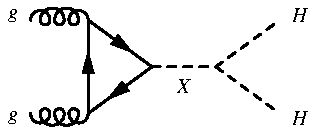
\includegraphics[width=0.8\textwidth]{feynman_graphs/di_higgs_resonant}

%     \column{0.6\textwidth}

%     \allbold{Search for scalars $X$ decaying to $HH$:}
%     \begin{itemize}
%       \setlength{\itemsep}{0.3em}
%     \item E.g.\ extended Higgs sector models
%     \item Mass range:\ $\SI{251}{\GeV} \leq m_{X} \leq \SI{1.6}{\TeV}$
%     %\item Negligible decay width
%     \end{itemize}
%   \end{columns}

% ------------------------------------------------------------------------------

\begin{frame}[standout]
  Constraining the Higgs Boson Self-Coupling

  \vspace*{1.5em}

  \hspace*{-7.5em}%
  \begin{overpic}[scale=1.0]{feynman_graphs/di_higgs_effective_inverted}
    \put(112,20){$\klambda = \lambda_{HHH} / \lambda_{HHH}^{\normalfont\text{SM}}$}
  \end{overpic}

  \begin{tikzpicture}[remember picture,overlay,shift=(current page.south
    west),x=(current page.south east),y=(current page.north west)]

    \draw[stealth-, line width=1pt, color=white] (0.443, 0.47) -- (0.443, 0.3)%
    node[align=center, below]{%
      \footnotesize New Physics?
    };
  \end{tikzpicture}
\end{frame}

% Notes: What if new physics changes the Higgs Boson self-coupling?
%
% - Heavy new particles might contribute (reduce to effective coupling)
%
% - Reinterpret the SM~\HH search \ra limits on xsec vs.\ $\kappa_{\lambda}$

% ------------------------------------------------------------------------------

% \begin{frame}{Constraining the Higgs Boson Self-Coupling}
% \end{frame}

% ------------------------------------------------------------------------------

\begin{frame}{Constraining the Higgs Boson Self-Coupling}
  \begin{columns}[onlytextwidth]
    \column{0.49\textwidth}

    \allbold{Reinterpretation of the SM~\HH search:}
    \begin{itemize}
      \setlength{\itemsep}{0.5em}
    \item Same background model \& discriminants
    \item Signal:~non-resonant \HH production with anomalous \klambda
    \end{itemize}

    \vspace*{1.5em}

    \onslide<3->{
      \allbold{\klambda constraints:}\\[-1.5\baselineskip]
      \begin{align*}
        \klambda &\in [-2.4, 9.2] \quad (\text{observed})\\
        \klambda &\in [-2.0, 9.0] \quad (b\text{-only expectation})
      \end{align*}
    }

    % \vspace*{1em}

    % {\footnotesize
    %   \textbf{Limitations:}\\
    %   Fixed single Higgs boson production cross sections \& Higgs boson
    %   branching ratios
    % }

    \column{0.02\textwidth}

    \column{0.49\textwidth} \centering

    \vspace*{0.1em}

    \onslide<2->{
      \allbold{Upper limits on $\sigma(pp \to HH)$ at~95\,\%~CL}

      \vspace*{0.7em}

      \begin{overpic}[width=0.95\textwidth]{self_coupling/klam_scan_result}
        \put(64,74){\tiny ATLAS-CONF-2021-052}
      \end{overpic}
      % Observed:~$\klambda \in [-2.4, 9.2]$
      % Expected:~$\klambda \in [-2.0, 9.0]$
    }
  \end{columns}

  % Limitations
  %
  % - Does not account for xsec / BR changes for single higgs
  %
  % - Not a statistically proper confidence interval
\end{frame}

% TODO: How are the cross section uncertainties treated when giving the limit?
%
% Looks like signal uncertainties are ignored, i.e. the limits are read off from
% the central value of the xsec prediction.

% ------------------------------------------------------------------------------

\begin{frame}[standout]
  Resonant \allbold{\HH} Production

  \vspace*{1.5em}

  \begin{overpic}[scale=1.0]{feynman_graphs/di_higgs_resonant_inverted}
  \end{overpic}
\end{frame}

% ------------------------------------------------------------------------------

% \begin{frame}{Resonant \allbold{\HH} Production}
%   \vspace*{0.1em}
%   \begin{columns}[onlytextwidth]
%     \column{0.5\textwidth}
%     \centering

%     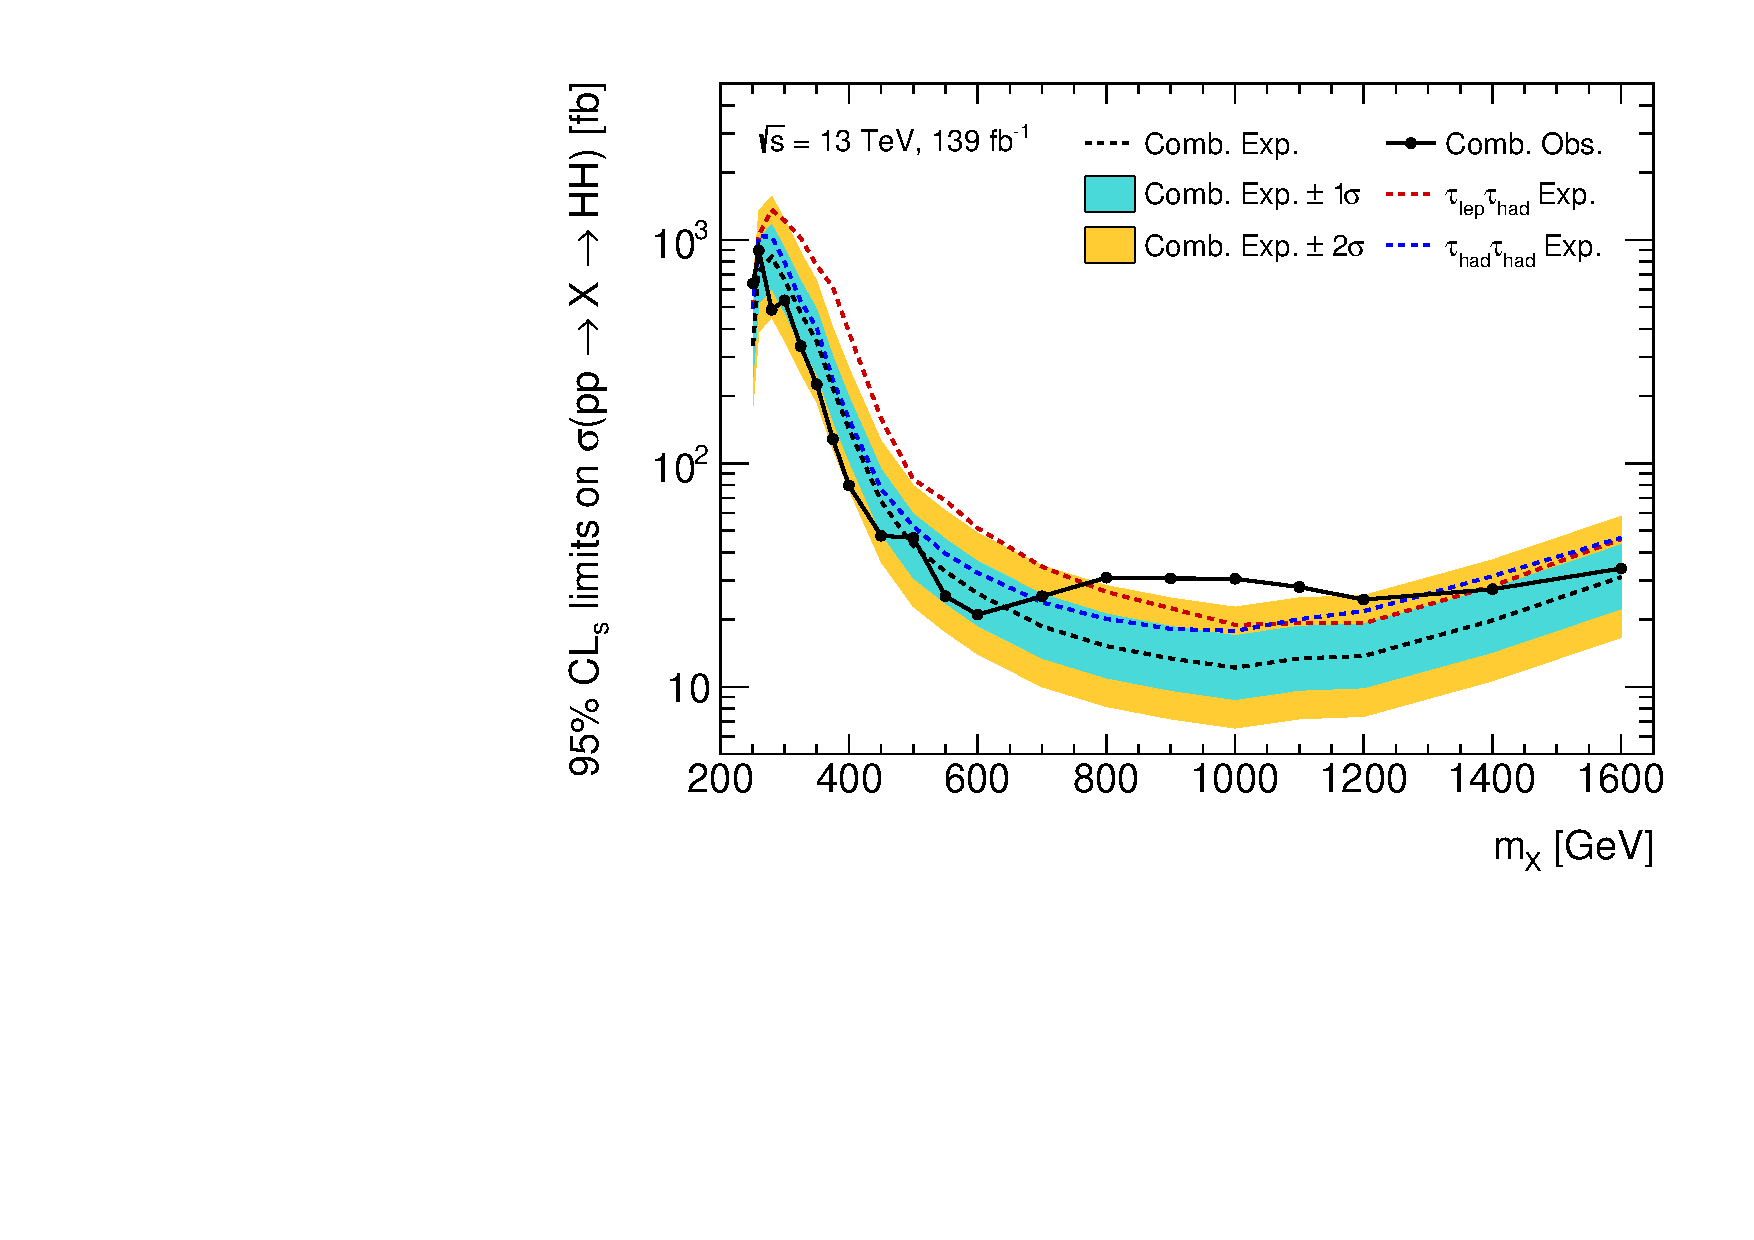
\includegraphics[width=0.9\textwidth]{results_res/resonant_upper_limits}

%     \column{0.5\textwidth}
%     \centering

%     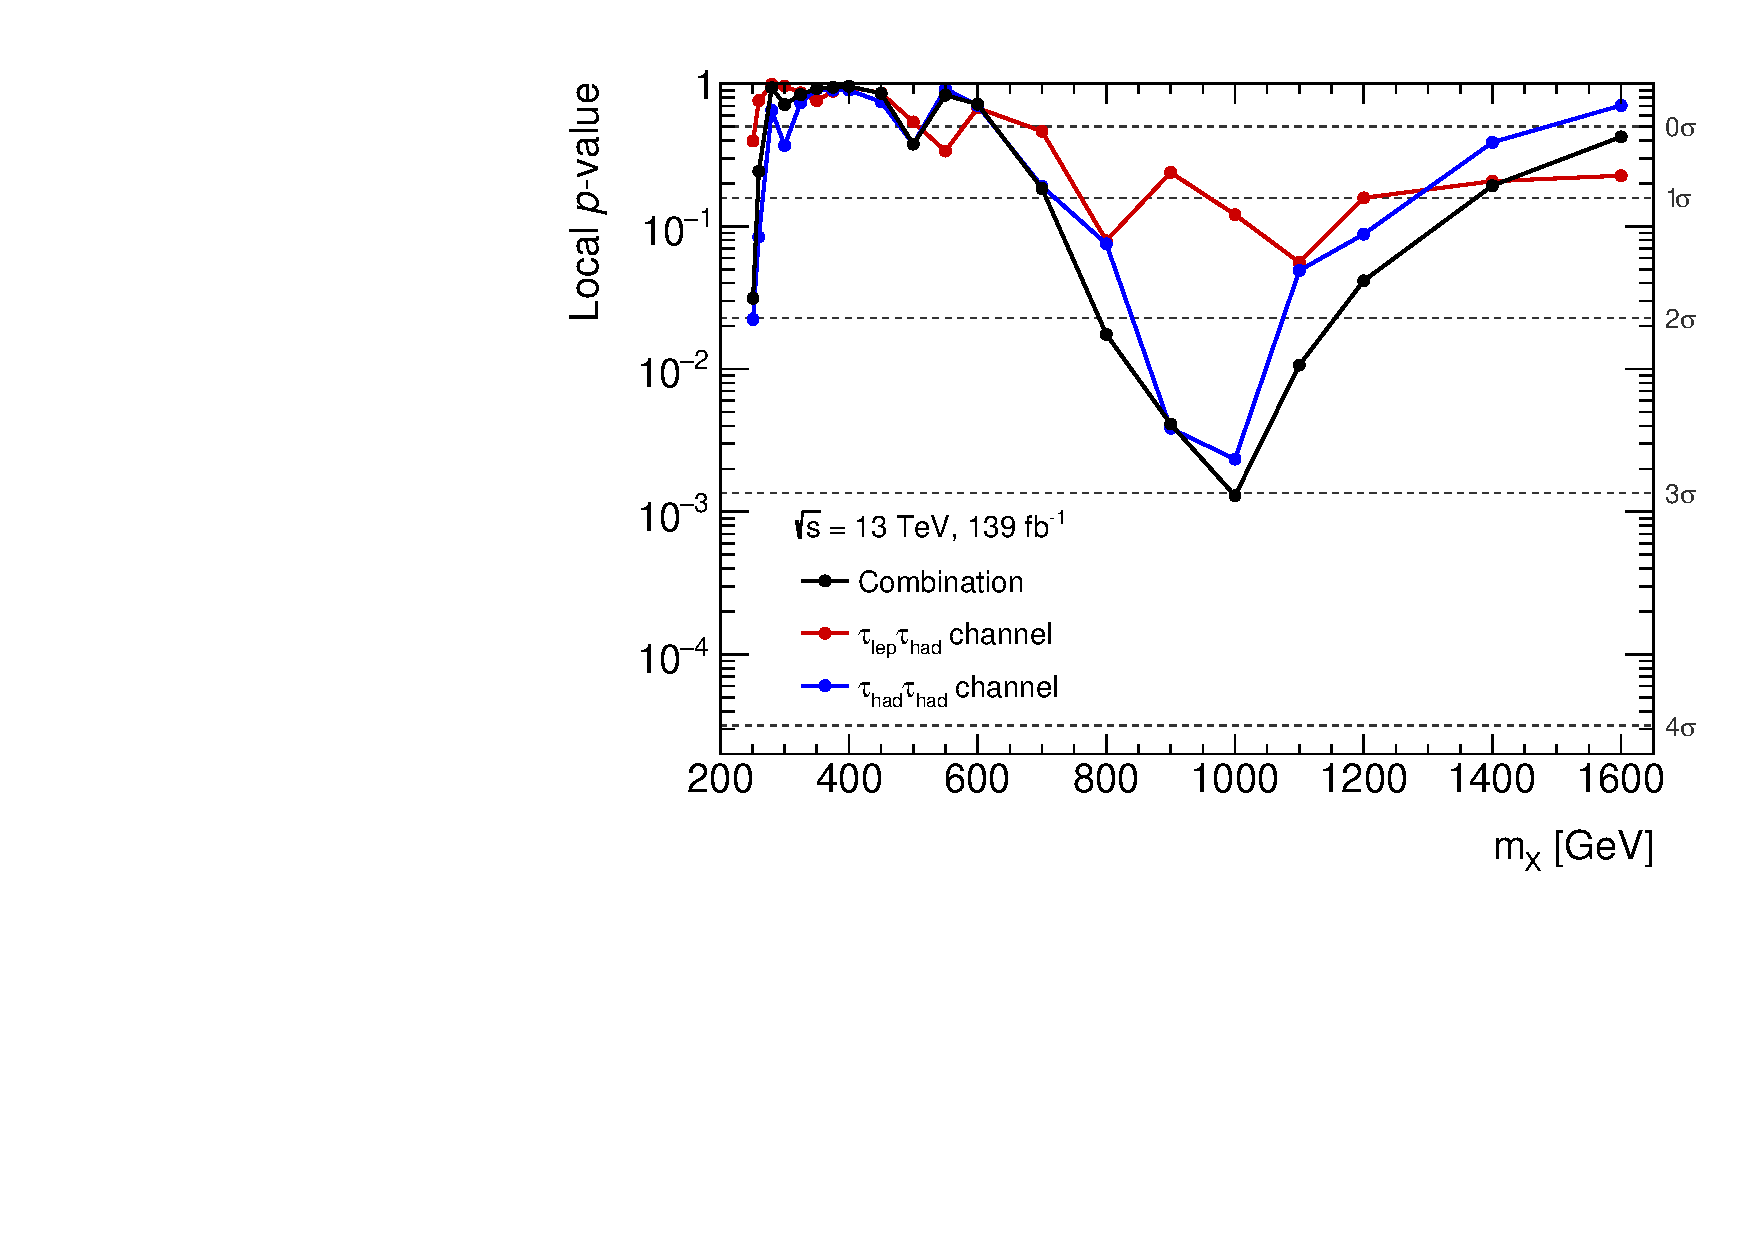
\includegraphics[width=0.9\textwidth]{results_res/resonant_comb_pvalues}
%   \end{columns}

%   Excess observed for $m_{X} = \SI{1000}{\GeV}$:
%   \begin{itemize}
%   \item Localised in \hadhad channel
%   \item Expect 6.3 background events but observed 14 events
%   \item Local (global) significance of $3.1\sigma$ ($2.0\sigma$)
%   \end{itemize}

%   Best fit xsec:
%   $\hat{\sigma}(pp \to X \to HH) = \left( 17.4^{+7.5}_{-6.5}
%   \right)\si{\femto\barn}$

%   \only<2>{%
%     \tikz[overlay, remember picture, shift=(current page.south west), x=(current
%     page.south east), y=(current page.north west), ]{ \node[align=center] at
%       (0.35,0.6) {%
%         \setlength{\fboxrule}{1pt}%
%         \fcolorbox{headergray}{mygray}{%
%           \begin{minipage}{0.333\textwidth}
%             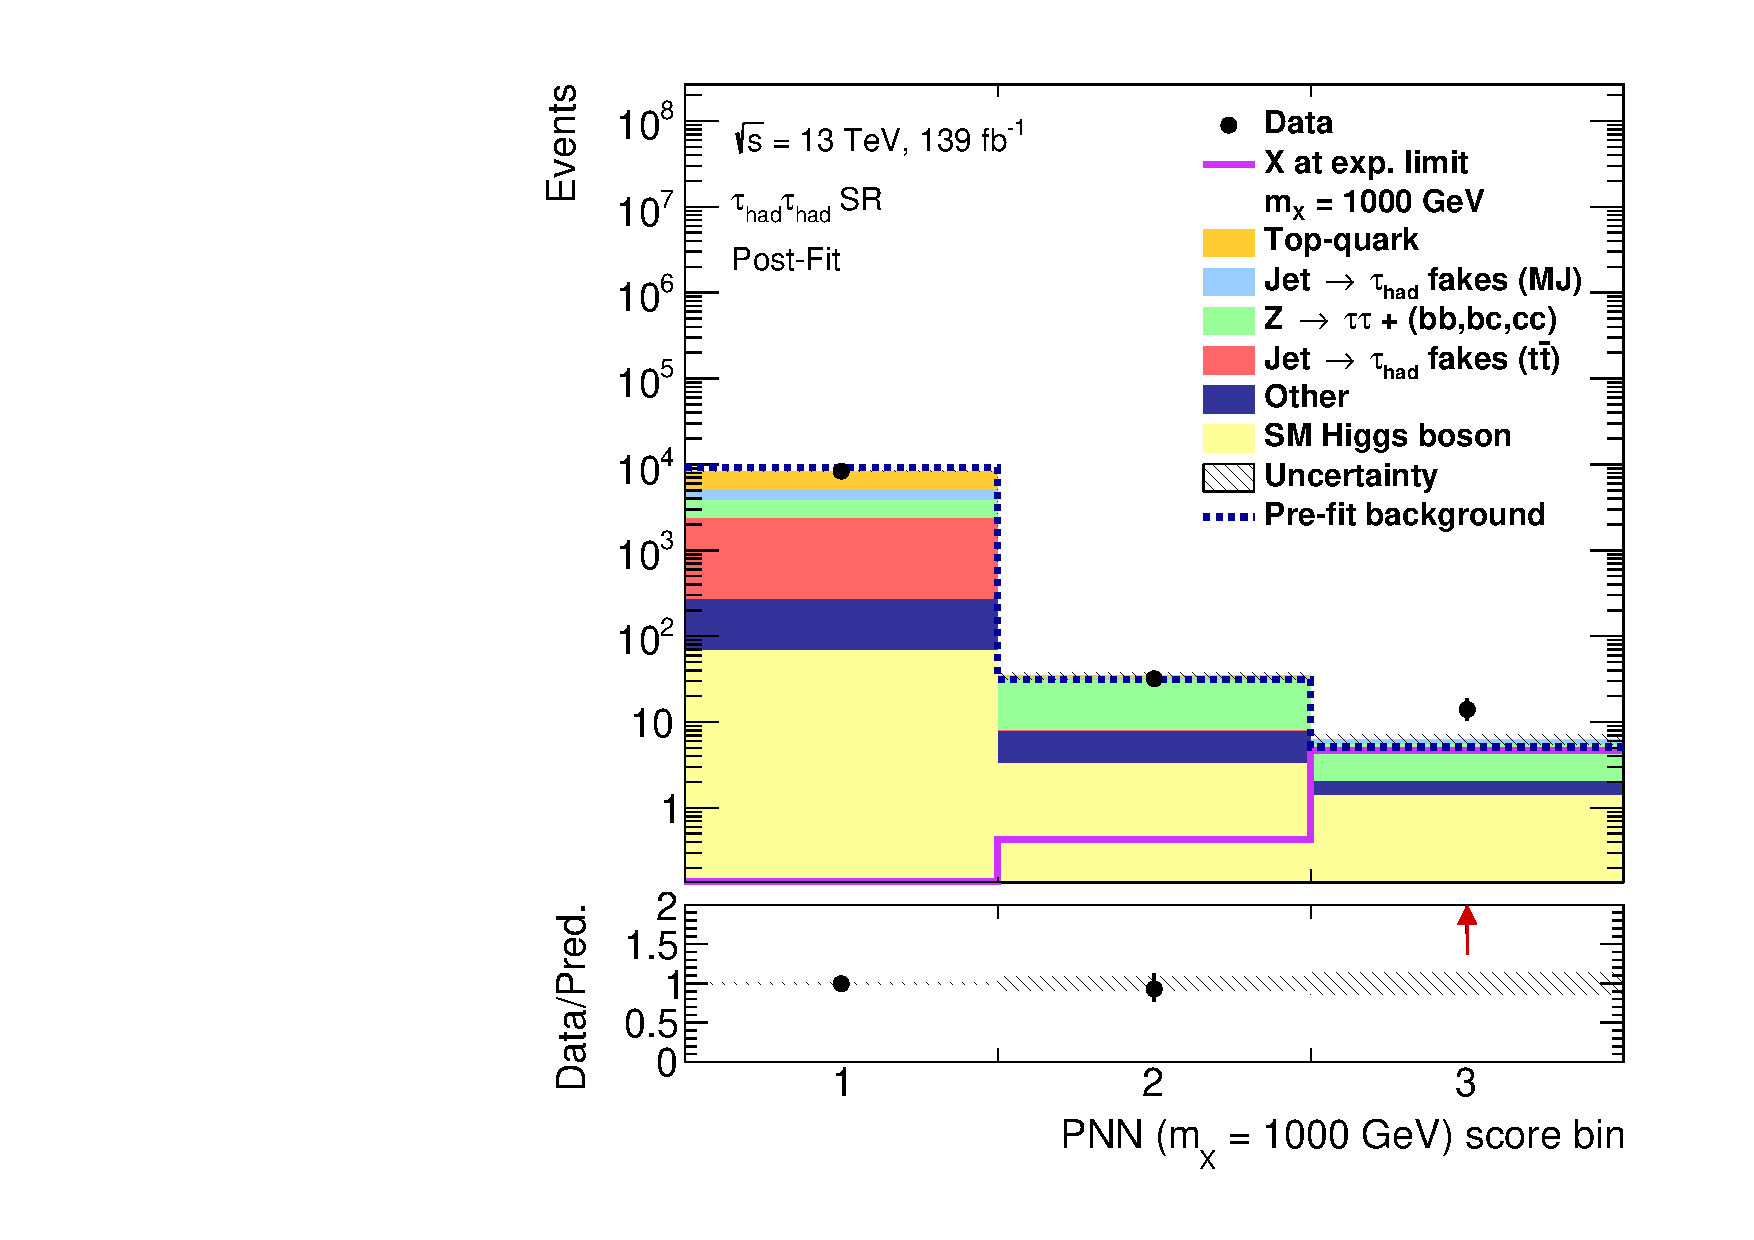
\includegraphics[width=\textwidth]{results_res/postfit/Region_BMin0_incJet1_distPNN1000_J2_Y2015_DLLOS_T2_SpcTauHH_L0_GlobalFit_conditionnal_mu0log}
%           \end{minipage}
%         }
%       };
%       \draw[-stealth, line width=1pt, color=Red] (0.44,0.554) -- (0.76,0.59);
%     }
%   }
% \end{frame}

% ------------------------------------------------------------------------------

% ------------------------------------------------------------------------------

\begin{frame}{Signal Extraction Revisited}
  \begin{columns}[onlytextwidth]
    \column{0.6\textwidth}

    \vspace*{0.2em}

    \textbf{Multiple signal hypotheses considered:}
    \begin{itemize}
    \item 20 mass points ($\SI{251}{\GeV} \leq m_{X} \leq \SI{1.6}{\TeV}$)
    \item Kinematic properties of signal changes with $m_{X}$
    \end{itemize}

    %\vspace*{0.75em}

    %\onslide<2->{\textbf{Previously:} 1 BDT per mass point}

    \vspace*{1.5em}

    %\onslide<2->{\textbf{Now:} Parameterised Neural Network (PNN)}
    \onslide<2->{\textbf{Parameterised Neural Network (PNN)}}


    \vspace*{1em}

    \onslide<2->{%
      \begin{overpic}[width=0.45\textwidth]{pnn_sketch}
        \put(85,25){\footnotesize \parbox[t]{0.47\textwidth}{Solves
            parameter-dependent classification problem}}
        \put(85,4){\tiny EPJC
          \textbf{77} (2016) 235}
      \end{overpic}
    }

    \column{0.4\textwidth}
    \centering

    \hspace*{1em}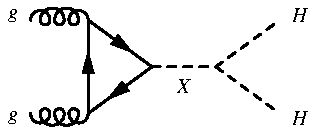
\includegraphics[width=0.75\textwidth]{feynman_graphs/di_higgs_resonant}

    \vspace*{2em}

    \hspace*{1em}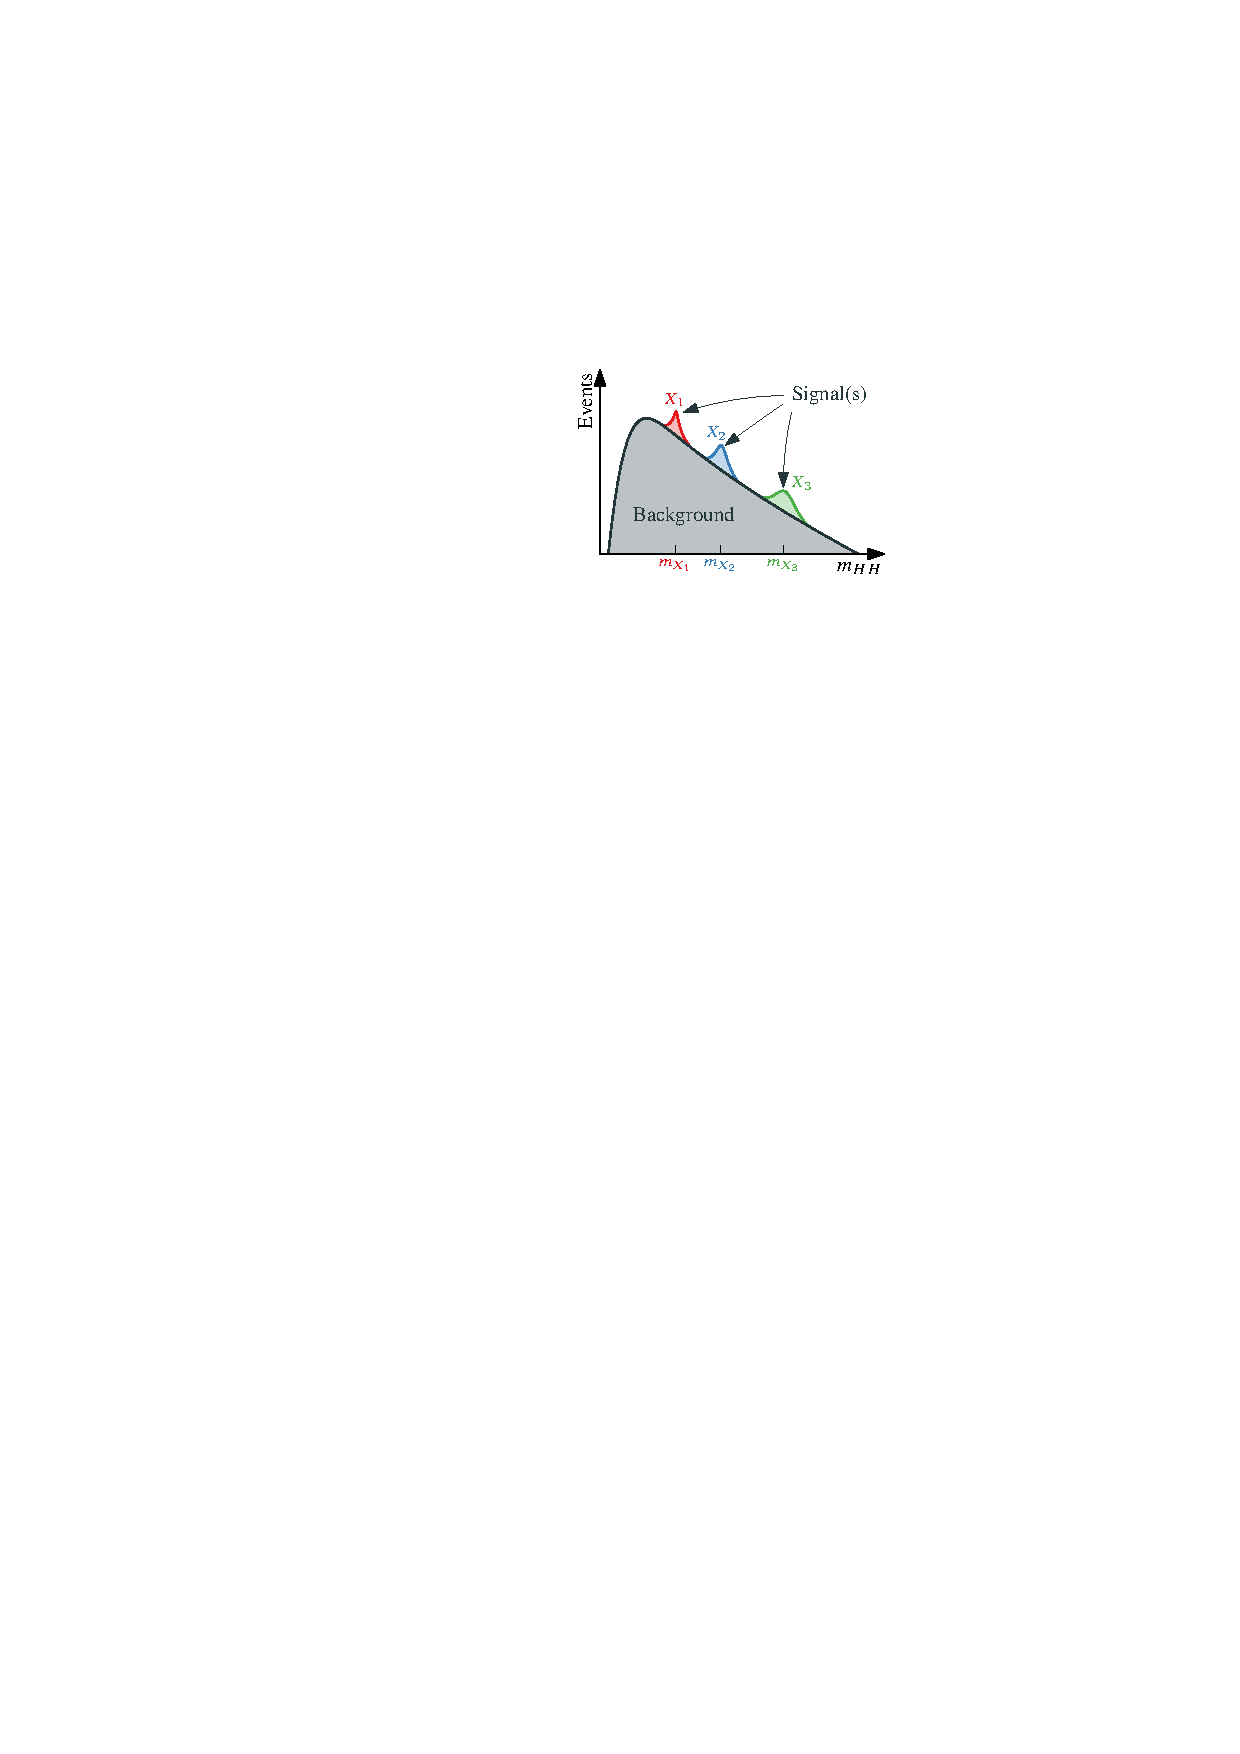
\includegraphics[width=0.95\textwidth]{resonant_signal_extraction_illustration}
  \end{columns}
\end{frame}

% ------------------------------------------------------------------------------

\begin{frame}{Discovery Tests (Resonant \allbold{\HH} Production)}
  \vspace*{0.5em}
  \begin{columns}[onlytextwidth, b]
    \column{0.5\textwidth}
    \centering

    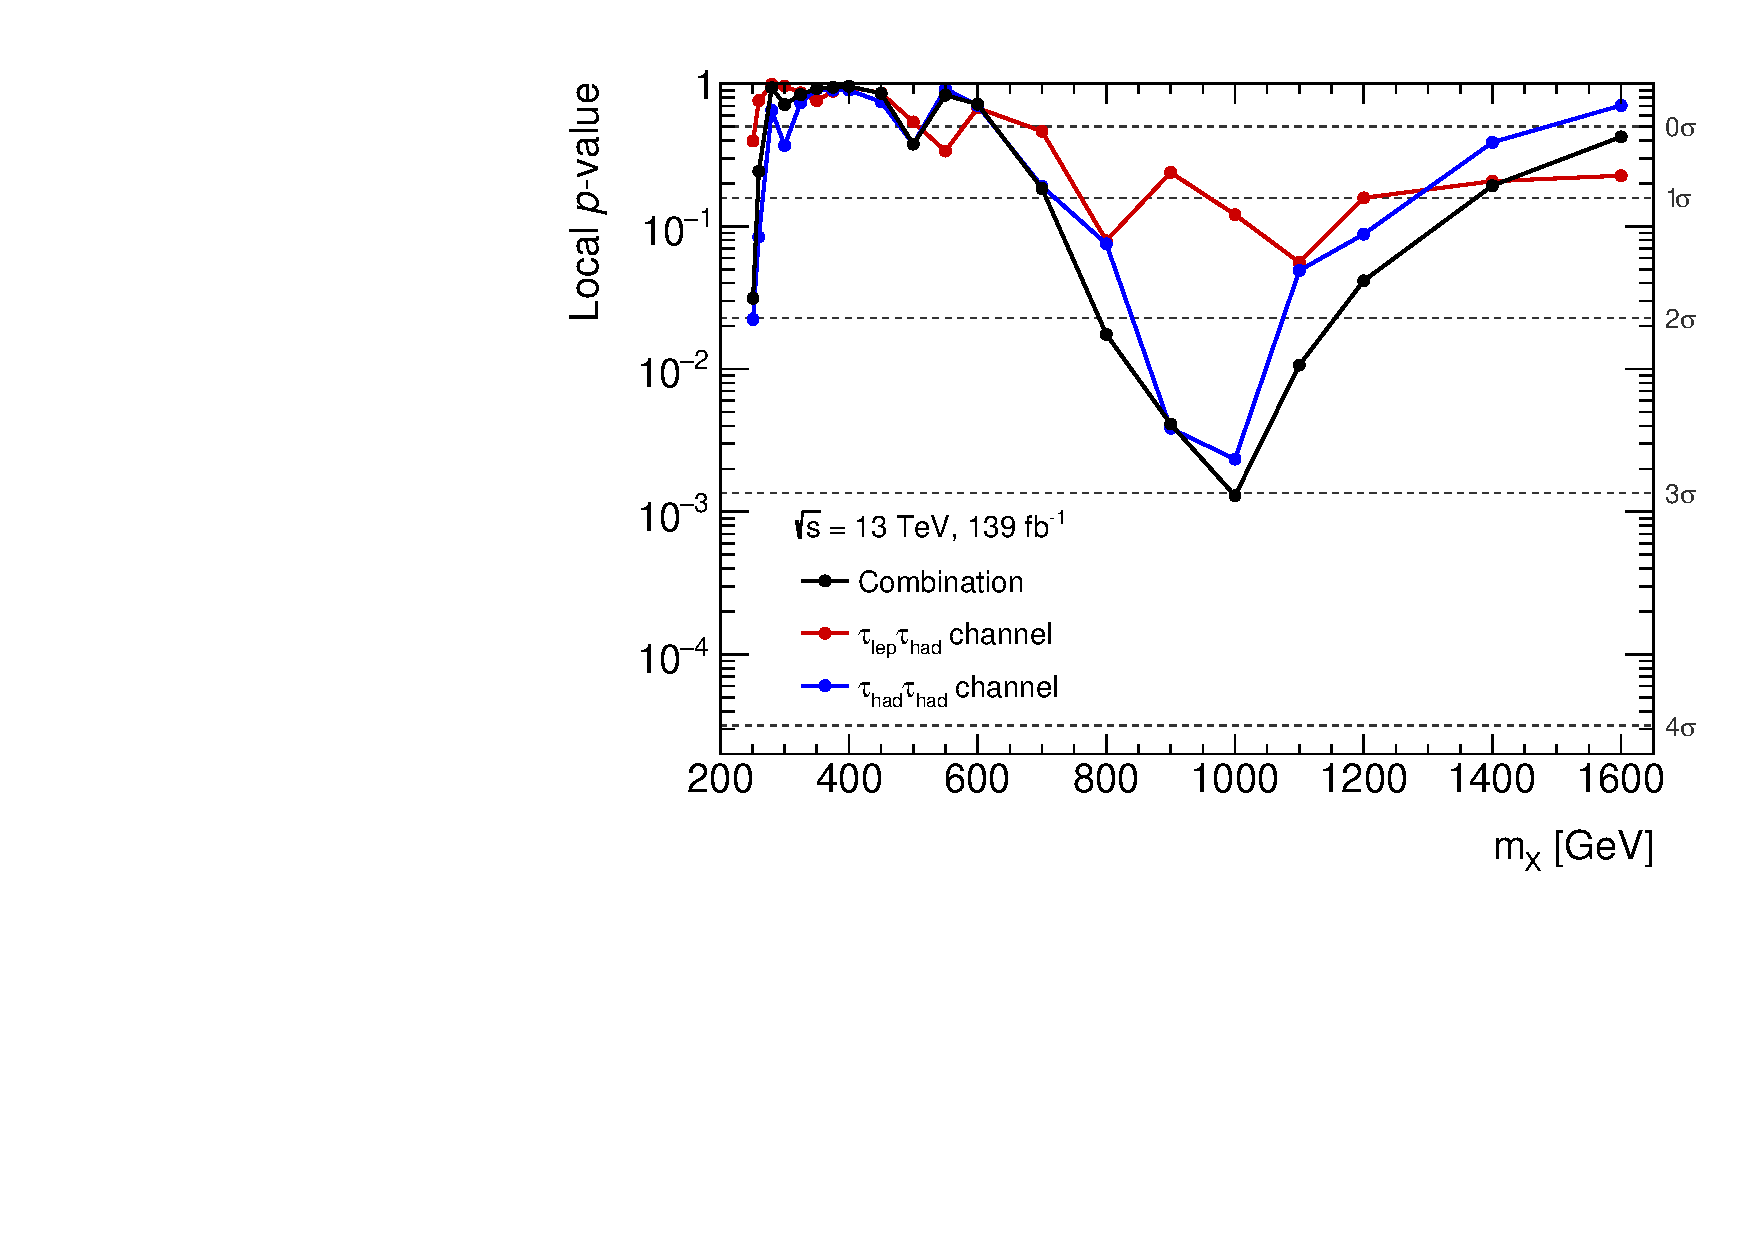
\includegraphics[width=1.0\textwidth, trim=0 0.3em 0 1em]{results_res/resonant_comb_pvalues}

    \column{0.5\textwidth}
    \centering

    \onslide<2->{%
      \hspace*{0.14\textwidth}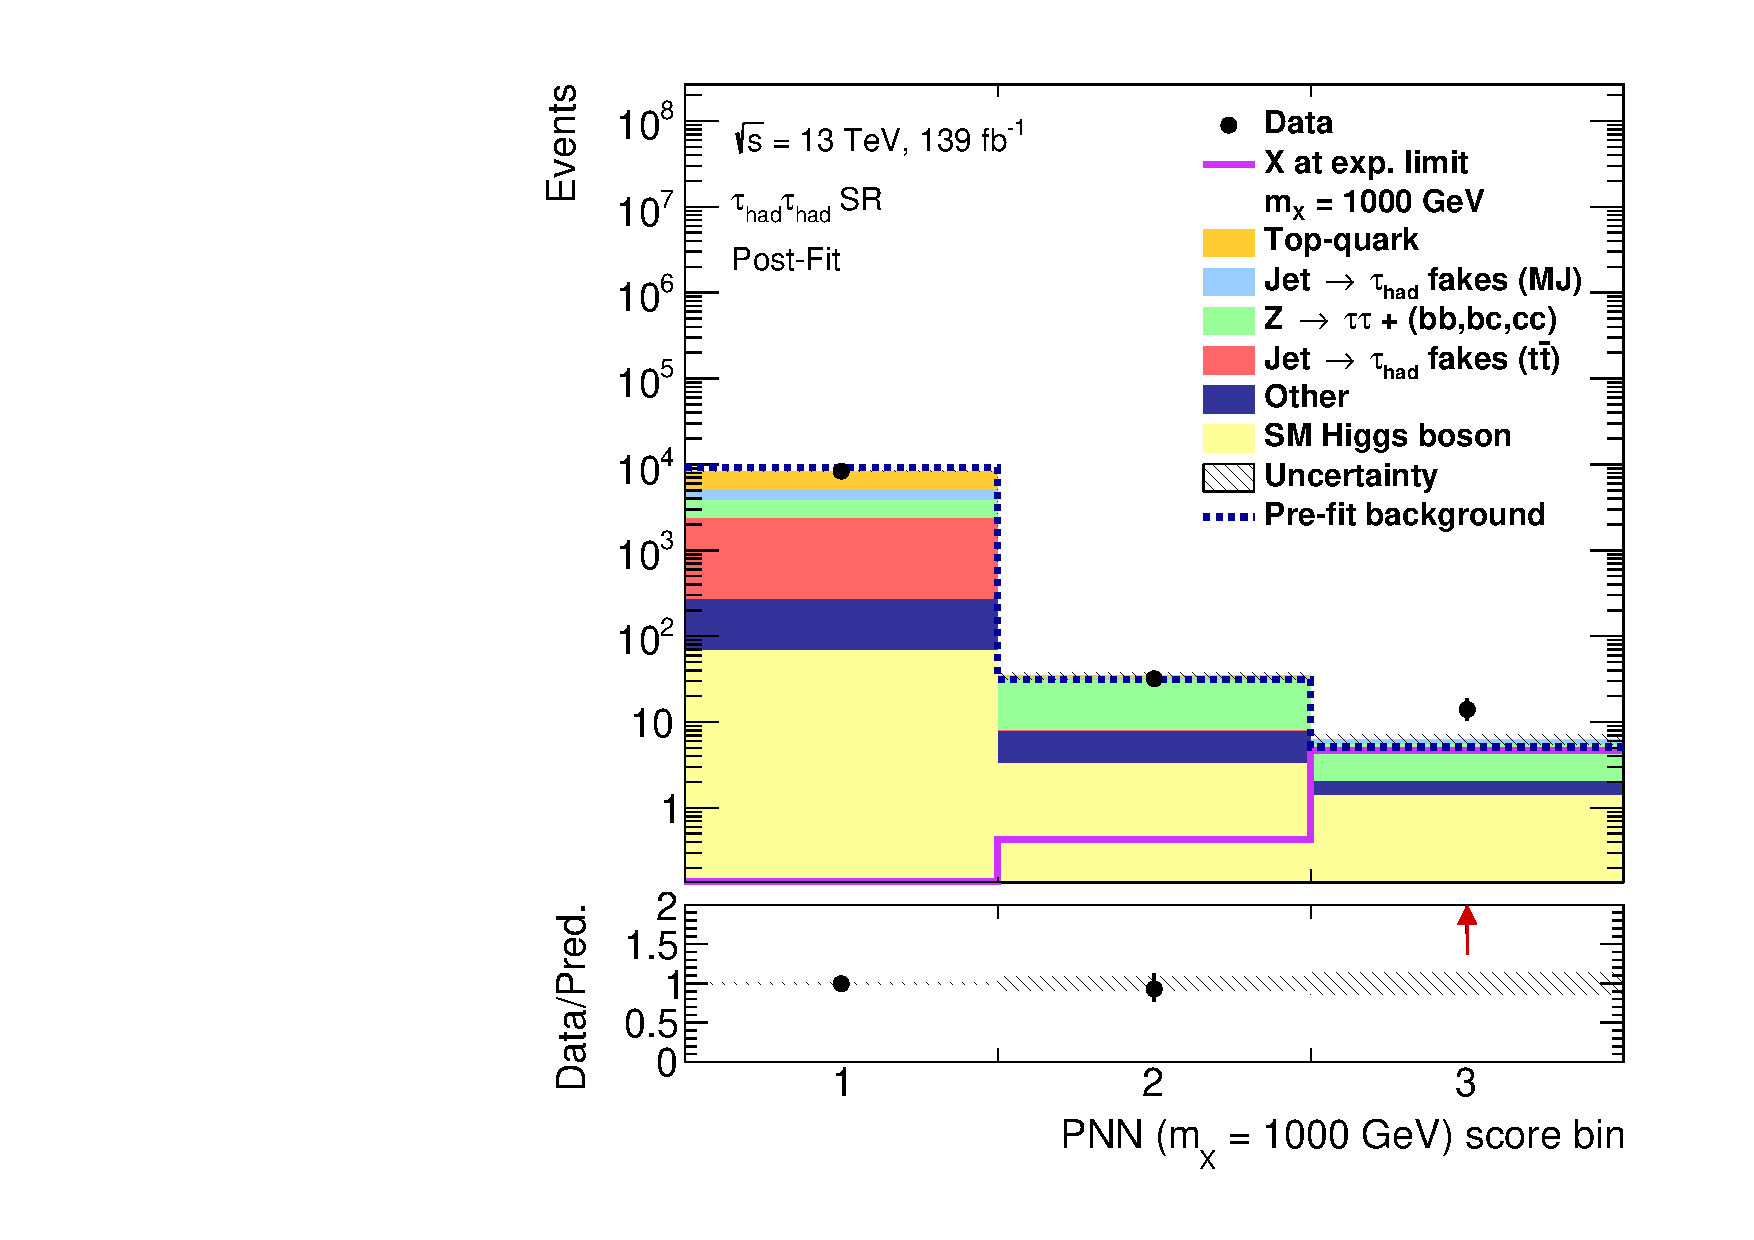
\includegraphics[width=0.75\textwidth, trim=0 0.3em 0 1em,
      clip]{results_res/postfit/Region_BMin0_incJet1_distPNN1000_J2_Y2015_DLLOS_T2_SpcTauHH_L0_GlobalFit_conditionnal_mu0log}
    }
  \end{columns}

  \vspace*{-0.1em}

  Excess observed at $m_{X} = \SI{1000}{\GeV}$\\[0.4em]
  \begin{itemize}
    \setlength{\itemsep}{0.4em}
  \item $\hat{\sigma}(pp \to X \to HH) = \left( 17.4^{+7.5}_{-6.5}
    \right)\si{\femto\barn}$
  \item Statistical significance: $3.1\sigma$ (local), $2.0\sigma$ (global)
  \end{itemize}

  \onslide<2->{%
    \tikz[overlay, remember picture, shift=(current page.south west), x=(current
    page.south east), y=(current page.north west), ]{
      \draw[-stealth, line width=1.5pt, color=Red] (0.33,0.55) -- (0.85,0.53);
      \node[anchor=west] at (0.91,0.54){\scriptsize\color{Red}Exp.:~6.3};
      \node[anchor=west] at (0.91,0.505){\scriptsize\color{Red}Obs.:~14};
    }
  }
\end{frame}

% ------------------------------------------------------------------------------

% \begin{frame}{Search for Resonant \allbold{\HH} Production: Upper Limits}
%   \vspace*{0.25em}
%   \begin{columns}
%     \column{0.5\textwidth}
%     \centering

%     \allbold{\bbtautau (all channels)}

%     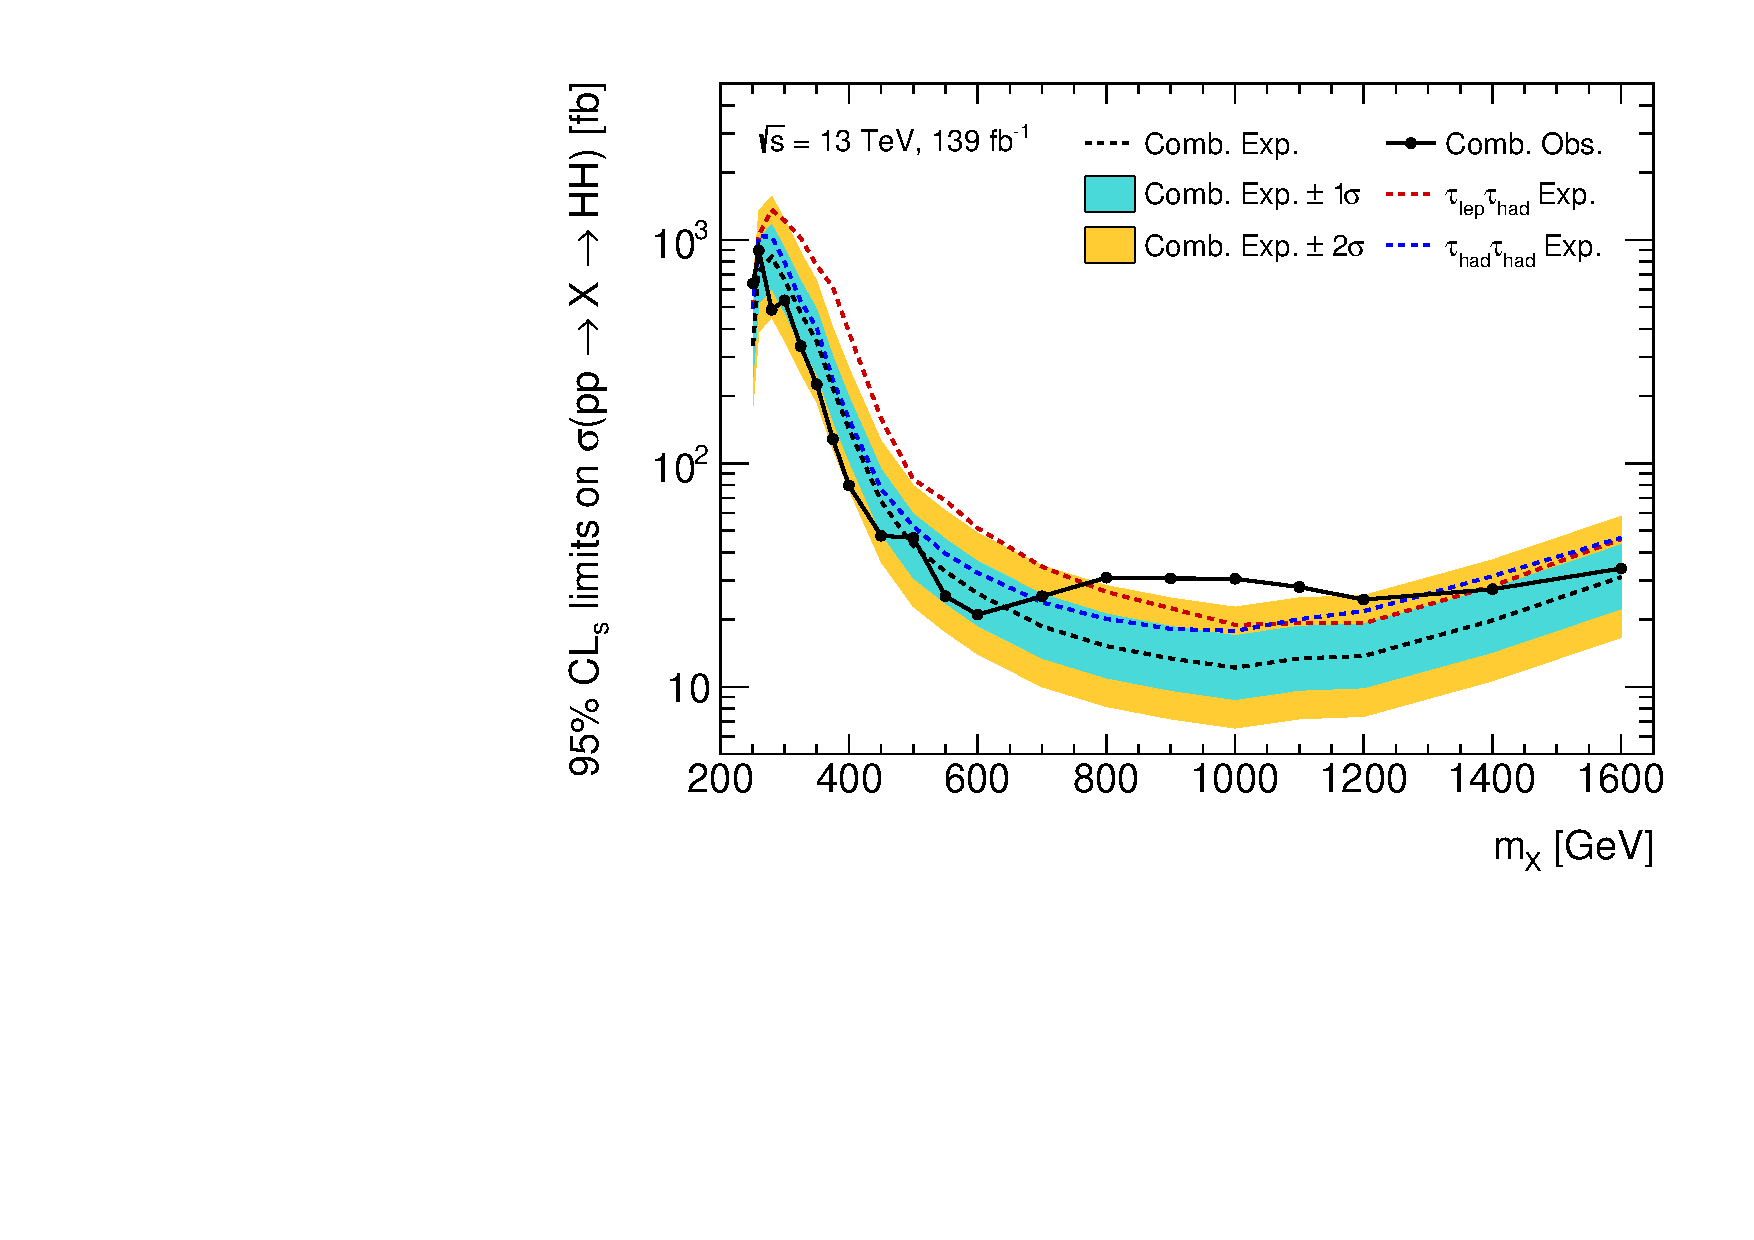
\includegraphics[width=\textwidth]{results_res/resonant_upper_limits}

%     \column{0.5\textwidth}
%     \centering

%     \allbold{\bbbb, \bbtautau and \bbyy (comparison)}

%     \includegraphics[width=\textwidth]{discussion/atlas_comparison_resonant_marked}
%   \end{columns}

%   \vspace*{0.2em}

%   \begin{itemize}
%     \setlength{\itemsep}{1em}

%     % \item Upper limits on $\sigma(pp \to X \to \HH)$ ranging from
%     %   \SI{20}{\femto\barn} to \SI{1000}{\femto\barn}

%   \item \bbtautau most sensitive channel in
%     $\SI{375}{\GeV} \leq m_{X} \leq \SI{800}{\GeV}$

%   \end{itemize}
% \end{frame}

\begin{frame}{Upper Limits (Resonant \allbold{\HH} Production)}
  \begin{center}
    \includegraphics[width=0.55\textwidth]{discussion/atlas_comparison_resonant_marked_without_obs}
  \end{center}

  \vspace*{-0.5em}

  \begin{itemize}
    \setlength{\itemsep}{1em}

  \item \bbtautau most sensitive channel in
    $\SI{375}{\GeV} \leq m_{X} \leq \SI{800}{\GeV}$

  \end{itemize}
\end{frame}

% ------------------------------------------------------------------------------




% ------------------------------------------------------------------------------

\begin{frame}{Summary \& Outlook}
  \begin{itemize}
    \setlength{\itemsep}{1em}

  \item Most sensitive search of \allbold{SM \HH production} to date
    % \begin{itemize}
    % \item $\mu_{HH} < 4.7$ (obs.) and $\mu_{HH} < 3.9$ (exp.) at 95\,\% CL
    % \end{itemize}

  \item Re-interpretation in the context of \allbold{anomalous \klambda}
    % \begin{itemize}
    % \item $\klambda \in [-2.4, 9.2]$ (obs.) and $\klambda \in [-2.0, 9.0]$ (exp.)
    % \end{itemize}

  \item Stringent contraints on \allbold{resonant \HH production} within
    $\SI{375}{\GeV} \leq \mX \leq \SI{800}{\GeV}$

  \end{itemize}

  \vspace*{1em}

  \textbf{Outlook:}
  \begin{itemize}
    \setlength{\itemsep}{1em}

  \item Re-analysis in progress -- stay tuned!

  \item First evidence of SM HH production expected at High-Luminosity LHC (2029
    -- 2041)

  \end{itemize}
\end{frame}

% ------------------------------------------------------------------------------

{ % all template changes are local to this group.
  \setbeamertemplate{navigation symbols}{}
  \setbeamercolor{background canvas}{bg=black}
  \begin{frame}<article:0>[plain]
    \begin{tikzpicture}[remember picture,overlay]
      \node[at=(current page.center)] {
        \includegraphics[keepaspectratio,
        width=\paperwidth,
        height=\paperheight]{event_displays/hadhad}
      };

      \node at (0.6\paperwidth,0.4\paperheight) {
        \huge \textcolor{White}{Thanks for your attention!}
      };
    \end{tikzpicture}
  \end{frame}
}

% ------------------------------------------------------------------------------

{ % all template changes are local to this group.
  \setbeamercolor{background canvas}{bg=black}
  \begin{frame}[plain]
    \begin{tikzpicture}[remember picture,overlay]
      \node[at=(current page.center)] {
        \includegraphics[keepaspectratio,
        width=\paperwidth,
        height=\paperheight]{event_displays/lephad}
      };
      % \node at (0.73\paperwidth,0.46\paperheight) {
      %   \textcolor{White}{$HH \ra {\color{bjetblue}b\bar{b}}{\color{taured}\tauhad\tauhad}$ candidate event}
      % };
    \end{tikzpicture}
  \end{frame}
}

% ------------------------------------------------------------------------------

\begin{frame}[standout]
  Backup
\end{frame}

% ------------------------------------------------------------------------------

\begin{frame}{Higgs Boson Production Cross Sections \& Branching Ratios}
  \begin{columns}[c]
    \column{0.5\textwidth}
    \centering

    \includegraphics[width=0.85\textwidth]{theory/h_prod_crossec_13tev}

    \column{0.5\textwidth}
    \centering\footnotesize

    \begin{tabular}{lS[table-format=2.3]c}
  \toprule
  Decay mode  & {BR / \%} & Observed \\
  \midrule
  $\bbbar$        & 58    & \checkmark \\
  $W^{+} W^{-}$    & 21    & \checkmark \\
  $gg$            & 8.2   & \\
  $\tau^+ \tau^-$ & 6.3   & \checkmark \\
  $c\bar{c}$      & 2.9   & \\
  $ZZ$            & 2.6   & \checkmark \\
  $\gamma\gamma$  & 0.23  & \checkmark \\
  $Z\gamma$       & 0.15  & \\
  $\mu^{+}\mu^{-}$ & 0.022 & $*$ \\
  \bottomrule
\end{tabular}

%%% Local Variables:
%%% mode: latex
%%% TeX-master: "../phd_thesis"
%%% End:


  \end{columns}

  {\footnotesize arXiv:1610.07922}
\end{frame}

% ------------------------------------------------------------------------------

\begin{frame}{Higgs Boson Pair Production:\ A Rare Process}

  \begin{columns}
    \column{0.35\textwidth}
    \centering

    % \begin{itemize}
    % \item Total proton--proton collision cross section:\ \SI{80}{\milli\barn}
    % \item W+jets: 20nb
    % \item ttbar: 831.76 pb
    % \item H: 48 pb (ggF) + 4 pb (VBF) (50pb)
    % \item HH: 31.05 + 1.726 = 32.8 fb
    % \item HHH: 80 ab (80e-18)
    % \end{itemize}
    \vspace*{1em} \includegraphics[width=0.95\textwidth]{cross_section_figure}

    \column{0.65\textwidth}

    \textbf{SM Expectation:}
    \vspace{0.5em}
    \begin{itemize}
      \setlength{\itemsep}{1em}

    \item 1 \HH event in 2.5 trillion inelastic collisions

    \item Total of 4000 \HH events produced in ATLAS from 2015--2018

      % Do not expect to find this in Run~2

    \end{itemize}
  \end{columns}
\end{frame}

% ------------------------------------------------------------------------------

\begin{frame}{Higgs Boson Pair Production in the SM}
  \vspace*{0.5em}

  \fbox{%
    \noindent\begin{minipage}{\dimexpr 0.25\textwidth - 2\fboxsep}
      \centering
      \textbf{Gluon--gluon fusion}\\[0.5\baselineskip]
      $\sigma_{\HH}^{gg\text{F}} = \SI{31}{\femto\barn}$
  \end{minipage}%
  \begin{minipage}{\dimexpr 0.75\textwidth - 2\fboxsep}
    \hspace*{0.1\textwidth}
    \includegraphics[scale=0.75]{feynman_graphs/di_higgs_box}%
    \hfill%
    \raisebox{0.35em}{\includegraphics[scale=0.75]{feynman_graphs/di_higgs_triangle}}%
    \hspace*{0.1\textwidth}
  \end{minipage}
  }

  \vspace*{2em}

  \fbox{%
    \noindent\begin{minipage}{\dimexpr 0.25\textwidth - 2\fboxsep}
      \centering
      \textbf{Vector boson fusion}\\[0.5\baselineskip]
      $\sigma_{\HH}^{\text{VBF}} = \SI{1.7}{\femto\barn}$
    \end{minipage}%
    \begin{minipage}{\dimexpr 0.75\textwidth - 2\fboxsep}
      \hspace*{0.04\textwidth}%
      \includegraphics[width=0.3\textwidth]{feynman_graphs/di_higgs_vbf_kvklam}%
      \hfill%
      \includegraphics[width=0.3\textwidth]{feynman_graphs/di_higgs_vbf_kvkv}%
      \hfill%
      \includegraphics[width=0.3\textwidth]{feynman_graphs/di_higgs_vbf_ktwov}%
      \hspace*{0.04\textwidth}
    \end{minipage}
  }

  \vspace*{1.0em}
  {\scriptsize In $pp$ collisions at $\sqrt{s} = \SI{13}{\TeV}$}
\end{frame}

% ------------------------------------------------------------------------------

\begin{frame}{Background Estimation: Overview}
  \begin{columns}
    \column{0.6\textwidth}

    \vspace*{1em}

    \resizebox{\textwidth}{!}{%
      \begin{tabular}{lcc}
        \toprule
        \allbold{Background} & \allbold{\hadhad channel} & \allbold{\lephad channel} \\
        \midrule
        $Z + \text{jets}$ & \multicolumn{2}{c}{\allbold{\textcolor{zjetsgreen}{Simulation (normalised in fit + dedicated CR)}}} \\[0.1em]
        \ttbar (true \tauhadvis) & \multicolumn{2}{c}{\textcolor{toporange}{Simulation (normalised in fit)}} \\[0.1em]
        \ttbar (fake \tauhadvis) & \allbold{\textcolor{topfakered}{Simulation + scale factors}} & \multirow{2}{*}{Fake factor method} \\[0.1em]
        Multi-jet & \allbold{\textcolor{fakeblue}{Fake factor method}} & \\[0.1em]
        Other & \multicolumn{2}{c}{Simulation} \\[0.1em]
        \bottomrule
      \end{tabular}
    }

    % \vspace*{1.5em}

    % {\footnotesize \textbf{Largest backgrounds in \hadhad channel:}
    %   \begin{itemize}
    %     \setlength{\itemindent}{0.75em}
    %   \item[1.] {\color{toporange}\ttbar with true-\tauhadvis} (\SI{39}{\percent} of bkg.)
    %   \item[2.] {\color{topfakered}\ttbar with fake-\tauhadvis} (\SI{25}{\percent} of bkg.)
    %   \item[3.] {\color{zjetsgreen}$Z + \text{jets}$} (\SI{18}{\percent} of bkg.)
    %   \item[4.] {\color{fakeblue}Multi-jet} (\SI{15}{\percent} of bkg.)
    %   \end{itemize}
    % }

    \column{0.4\textwidth}

    \vspace*{1.5em}

    \begin{overpic}[width=\textwidth]{results_nonres/postfit_mvainputs/Region_BMin0_incJet1_distmHH_J2_Y2015_DLLOS_T2_SpcTauHH_L0_GlobalFit_conditionnal_mu0log}
      %\put(56,94){\tiny arXiv:2209.10910}
    \end{overpic}
  \end{columns}

  % Dominant backgrounds:
  % Z+jets: 18\,\%
  % Top quark: 39\,\%
  % fakes (ttbar + multijet): 40\,\%

  % Dominant backgrounds:
  % ttbar: 62\,\%
  % Fakes: 34\,\%
  % Z+jets: 2\,\%
\end{frame}

% ------------------------------------------------------------------------------

\begin{frame}{Background Estimation: \allbold{$Z + \text{jets}$}}
  $Z$ + heavy-flavour jets normalised in fit using CR targeting $\ell^+\ell^-$ +
  2 $b$-tagged jets

  \begin{center}
    \begin{tikzpicture}
      \node (prefit) at (0,0) {
        \includegraphics[width=0.4\textwidth]{zhfcr/Region_BMin0_incJet1_Y2015_DZllbbCR_T2_L2_distmLL_J2_Prefit_fixed}
      };

      \node[anchor=west,fill=white] at (-2.1,1.7){\footnotesize \allbold{Pre-Fit}};

      \onslide<2->{%
        \node (postfit) at (8,0) {
          \includegraphics[width=0.4\textwidth]{zhfcr/Region_BMin0_incJet1_Y2015_DZllbbCR_T2_L2_distmLL_J2_GlobalFit_conditionnal_mu0_fixed}
        };

        \draw[-stealth, line width=1.5pt] (2,0) -- node[below,midway]{\footnotesize $Z$+HF SF
          $\approx 1.4$} node[above,midway]{\footnotesize CR only fit} (6.2,0);

        \node[anchor=west,fill=white] at (5.9,1.7){\footnotesize \allbold{Post-Fit}};
      }
    \end{tikzpicture}
  \end{center}
\end{frame}

% ------------------------------------------------------------------------------

\begin{frame}{Background Estimation: \allbold{\ttbar} with Fake
    \allbold{\tauhadvis}}
  \begin{columns}[onlytextwidth]
    \column{0.55\textwidth}

    \textbf{Data-driven corrections} applied to simulated \ttbar events with fake
    \tauhadvis.

    \vspace*{2em}

    \allbold{Measured in a $\ell + \tauhadvis$~CR} %in bins of:\ \tauhadvis~\pT,
    %\tauhadvis~\Ntracks, \tauhadvis-trigger.

    \vspace*{2em}

    \mtw to distinguish fake- from true-\tauhadvis.

    \column{0.45\textwidth}
    \centering

    \vspace*{0.1em}

    \begin{tikzpicture}

      \node[anchor=south west] (image) at (0,0) {
        \includegraphics[width=\textwidth]{ttbarSF/postfit_sfcr/MTWVR_postFit}
      };

      \draw[stealth-, line width=1.5pt] (2.6,3.5) -- (2.6,4.65)
      node[above,black,]{\footnotesize \ttbar + true \tauhadvis};

      \draw[stealth-, line width=1.5pt] (2.6,2.3) -- (3.9,3.4) node[above
      right,black]{\footnotesize \ttbar + fake \tauhadvis};

    \end{tikzpicture}

    {\footnotesize
      $\mtw = \sqrt{ 2 \, \pT^\ell \, \pTmissAbs \, (1 - \cos\Delta\phi)}$
    }
  \end{columns}
\end{frame}

% ------------------------------------------------------------------------------

\begin{frame}{Background Estimation: Multi-Jet}
  \begin{columns}[onlytextwidth]
    \column{0.65\textwidth}

    \textbf{Multi-jet-enriched CRs defined using:}
    \begin{itemize}
      \setlength{\itemsep}{0.5em}

    \item \allbold{\tauhadvis charge:}\ opposite sign, same sign

    \item \allbold{\tauhadvis identification:}\ 2 loose \tauhadvis, \\1 loose
      \tauhadvis \& 1 anti-\tauhadvis

    \end{itemize}

    \column{0.35\textwidth}

    \vspace*{1em}

    \hfill\includegraphics[width=0.92\textwidth]{ff_sketch}

  \end{columns}

  \onslide<1->{%
    \textbf{Fake factor method:}\\[-1em]
    \begin{flalign*}
      \qquad N_\text{A} &= {\color{Red}\frac{N_\text{C}}{N_\text{D}}} \cdot N_\text{B}
      = {\color{Red}\text{FF}} \cdot N_\text{B} &
    \end{flalign*}

    \vspace*{-0.25em}

    % \begin{itemize}
    %   \setlength{\itemsep}{0.5em}

    % \item FF binned in \tauhadvis properties, trigger, data-taking period

    % \item FF measured in 1 $b$-tag region and extrapolated to 2 $b$-tag region

    % \end{itemize}
  }

  % Details for backup:\\
  % - Actually do two different fake estimations and average\\

  \onslide<3->{%
    \setlength{\fboxrule}{1pt}
    \begin{tikzpicture}[remember picture,overlay,shift=(current page.south
      west),x=(current page.south east),y=(current page.north west)]

      \filldraw[white,opacity=0.7](0.0,0.08) rectangle (0.6,0.87);

      \node[align=center] at (0.43,0.5){%
        \fcolorbox{headergray}{white}{\includegraphics[width=0.4\textwidth]{fakefactors/fake_os_vr/Tau0Pt_fakevr}}
      };

      \node[align=center] at (0.45,0.5){%
        \textbf{Multi-Jet VR}};

      \draw[stealth-, line width=1.5pt, red] (0.6,0.6) -- (0.81,0.6);
    \end{tikzpicture}
  }
\end{frame}

% ------------------------------------------------------------------------------

\begin{frame}{Results:\ Early Run~2 Analyses (SM~\allbold{\HH})}
  \begin{columns}
    \column{0.5\textwidth}\centering\footnotesize

    \includegraphics[width=\textwidth]{status/atlas_36ifb}

    Phys.\ Lett.\ B \textbf{800} (2020) 135103

    \column{0.5\textwidth}\centering\footnotesize

    \includegraphics[width=\textwidth]{status/cms_36ifb}

    Phys.\ Rev.\ Lett.\ \textbf{122} (2019) 121803
  \end{columns}
\end{frame}

% ------------------------------------------------------------------------------

\begin{frame}{Results:\ Early Run~2 Analyses (Resonant \allbold{\HH}
    Production)}
  \begin{columns}
    \column{0.45\textwidth}\centering\footnotesize

    \includegraphics[width=\textwidth]{status/atlas_36ifb_resonant}

    Phys.\ Lett.\ B \textbf{800} (2020) 135103

    \column{0.55\textwidth}\centering\footnotesize

    \includegraphics[width=\textwidth]{status/cms_36ifb_resonant}

    Phys.\ Rev.\ Lett.\ \textbf{122} (2019) 121803
  \end{columns}
\end{frame}

% ------------------------------------------------------------------------------

\begin{frame}{Results:\ Early Run~2 Analyses (Anomalous \allbold{\klambda})}
  \begin{columns}
    \column{0.5\textwidth}\centering\footnotesize

    \includegraphics[width=\textwidth]{status/atlas_36ifb_klambda}

    Phys.\ Lett.\ B \textbf{800} (2020) 135103

    \column{0.5\textwidth}\centering\footnotesize

    \includegraphics[width=\textwidth]{status/cms_36ifb_klambda}

    Phys.\ Rev.\ Lett.\ \textbf{122} (2019) 121803
  \end{columns}
\end{frame}

% ------------------------------------------------------------------------------

\begin{frame}{Tau Lepton Decay}
  \begin{columns}
    \column{0.5\textwidth}\centering\footnotesize

    \includegraphics[width=0.7\textwidth]{tauid/tau_decay_feynman}

    \column{0.5\textwidth}\centering\footnotesize

    \includegraphics[width=0.9\textwidth]{tauid/tau_branching_pie_chart_new}
  \end{columns}
\end{frame}

% ------------------------------------------------------------------------------

\begin{frame}{Long Short-Term Memory}
  \centering\footnotesize

  \includegraphics[width=0.6\textwidth]{ml/lstm}

  \begin{columns}
    \column{0.5\textwidth}\footnotesize

    \begin{alignat*}{4}
      &\myvec{f}_{t} &&= \myvec{\sigma}\bigl(\myvec{U}^{\text{f}}  \myvec{x}_{t} &&+ \myvec{W}^{\text{f}}  \myvec{y}_{t - 1} &&+ \myvec{b}^{\text{f}}\bigr) \\
      &\myvec{i}_{t} &&= \myvec{\sigma}\bigl(\myvec{U}^{\text{i}}  \myvec{x}_{t} &&+ \myvec{W}^{\text{i}}  \myvec{y}_{t - 1} &&+ \myvec{b}^{\text{i}}\bigr) \\
      &\myvec{o}_{t} &&= \myvec{\sigma}\bigl(\myvec{U}^{\text{o}}  \myvec{x}_{t} &&+ \myvec{W}^{\text{o}}  \myvec{y}_{t - 1} &&+ \myvec{b}^{\text{o}}\bigr)
    \end{alignat*}

    \column{0.5\textwidth}\footnotesize

    \begin{align*}
      \myvec{s}_{t} = \myvec{f}_{t} \circ \myvec{s}_{t - 1}
      + \myvec{i}_{t} \circ \myvec{\phi}(\myvec{U} \myvec{x}_{t} + \myvec{W} \myvec{y}_{t-1} + \myvec{b})
    \end{align*}
  \end{columns}
\end{frame}

% ------------------------------------------------------------------------------

\begin{frame}[standout]
  Tau Identification
\end{frame}

% ------------------------------------------------------------------------------

\begin{frame}{Tau Identification:\ Simulated \tauhadvis Candidate Samples}
  \begin{columns}
    \column{0.5\textwidth}\centering\footnotesize

    \allbold{$\gamma^* \to \tau^+\tau^-$}

    \includegraphics[width=0.9\textwidth]{tauid/pubnote/taupt_gammastar}

    \column{0.5\textwidth}\centering\footnotesize

    \allbold{Di-jet}

    \includegraphics[width=0.9\textwidth]{tauid/pubnote/taupt_dijet}
  \end{columns}

  \footnotesize

  \# true \tauhadvis candidates:\ 20 million

  \# fake \tauhadvis candidates:\ 46 million
\end{frame}

% ------------------------------------------------------------------------------

\begin{frame}{Tau Identification:\ Input Variables (High-Level Inputs)}
  \centering

  \includegraphics[width=0.8\textwidth, trim=0 3.7in 0 0,
  clip]{backup/tauid_variable_table}
\end{frame}

% ------------------------------------------------------------------------------

\begin{frame}{Tau Identification:\ Input Variables (High-Level Inputs)}
  \centering

  \includegraphics[width=0.33\textwidth]{tauid/invars/invars_sumpttrkfrac_1P}%
  \includegraphics[width=0.33\textwidth]{tauid/invars/invars_ptratioeflowapprox_1P}%
  \includegraphics[width=0.33\textwidth]{tauid/invars/invars_masstrksys_3P}
\end{frame}

% ------------------------------------------------------------------------------

\begin{frame}{Tau Identification:\ Input Variables (Track inputs)}
  \centering

  \includegraphics[width=0.8\textwidth, trim=0 1.55in 0 3.5in,
  clip]{backup/tauid_variable_table}
\end{frame}

% ------------------------------------------------------------------------------

\begin{frame}{Tau Identification:\ Input Variables (Track inputs)}
  \centering

  \includegraphics[width=0.33\textwidth]{tauid/invars/invars_trk0relpt_1P}%
  \includegraphics[width=0.33\textwidth]{tauid/invars/invars_trk1relpt_1P}%
  \includegraphics[width=0.33\textwidth]{tauid/invars/invars_trk2relpt_1P}
\end{frame}

% ------------------------------------------------------------------------------

\begin{frame}{Tau Identification:\ Input Variables (Track inputs)}
  \centering

  \begin{overpic}[width=0.57\textwidth]{backup/track_2d_1P}
    \put(-20,22){1-prong}
  \end{overpic}

  \vspace*{-0.75em}

  \begin{overpic}[width=0.57\textwidth]{backup/track_2d_3P}
    \put(-20,22){3-prong}
  \end{overpic}
\end{frame}

% ------------------------------------------------------------------------------

\begin{frame}{Tau Identification:\ Input Variables (Cluster Inputs)}
  \centering

  \includegraphics[width=0.8\textwidth, trim=0 0 0 5.7in,
  clip]{backup/tauid_variable_table}
\end{frame}

% ------------------------------------------------------------------------------

\begin{frame}{Tau Identification:\ Input Variables (Cluster Inputs)}
  \centering

  \includegraphics[width=0.33\textwidth]{tauid/invars/invars_cls0relet_3P}%
  \includegraphics[width=0.33\textwidth]{tauid/invars/invars_cls1relet_3P}%
  \includegraphics[width=0.33\textwidth]{tauid/invars/invars_cls2relet_3P}
\end{frame}

% ------------------------------------------------------------------------------

\begin{frame}{Tau Identification:\ Input Variables (Cluster inputs)}
  \centering

  \begin{overpic}[width=0.57\textwidth]{backup/cluster_2d_1P}
    \put(-20,22){1-prong}
  \end{overpic}

  \vspace*{-0.75em}

  \begin{overpic}[width=0.57\textwidth]{backup/cluster_2d_3P}
    \put(-20,22){3-prong}
  \end{overpic}
\end{frame}

% ------------------------------------------------------------------------------

\begin{frame}{Tau Identification:\ Architecture}
  \begin{center}
    \includegraphics[width=0.9\textwidth]{tauid/pubnote/rnn_network_architecture}
  \end{center}

  \begin{itemize}
    \setlength{\itemsep}{0.5em}

  \item \num{56000} trainable parameters

  \item High-level variable branch:\ 128, 128, 16 nodes

  \item Track/cluster branches:\ 32, 32 nodes -- 32, 24 nodes for the LSTM
    internal state

  \item After merge:\ 64, 32, 1 nodes

  \end{itemize}
\end{frame}

% ------------------------------------------------------------------------------

\begin{frame}{Tau Identification:\ RNN Scores}
  \includegraphics[width=0.5\textwidth]{tauid/rnnscore_1p}%
  \includegraphics[width=0.5\textwidth]{tauid/rnnscore_3p}

  \begin{itemize}
  \item Output score is flattened w.r.t.\ $\mu$ and \tauhadvis $\pT$
  \end{itemize}
\end{frame}

% ------------------------------------------------------------------------------

\begin{frame}{Tau Identification:\ Rejection Table}
  \centering

  \includegraphics[width=0.8\textwidth]{backup/tauid_rejection}
\end{frame}

% ------------------------------------------------------------------------------

\begin{frame}{Tau Identification:\ Efficiency/Rejection vs.\ \allbold{\pT}}
  \centering

  \includegraphics[width=0.35\textwidth]{tauid/pubnote/eff_vs_pt_1p}%
  \includegraphics[width=0.35\textwidth]{tauid/pubnote/eff_vs_pt_3p}%

  \includegraphics[width=0.35\textwidth]{tauid/pubnote/rej_vs_pt_1p}%
  \includegraphics[width=0.35\textwidth]{tauid/pubnote/rej_vs_pt_3p}%
\end{frame}

% ------------------------------------------------------------------------------

\begin{frame}{Tau Identification:\ Efficiency/Rejection vs.\ \allbold{$\eta$}}
  \centering

  \includegraphics[width=0.35\textwidth]{tauid/pubnote/eff_vs_eta_1p}%
  \includegraphics[width=0.35\textwidth]{tauid/pubnote/eff_vs_eta_3p}%

  \includegraphics[width=0.35\textwidth]{tauid/pubnote/rej_vs_eta_1p}%
  \includegraphics[width=0.35\textwidth]{tauid/pubnote/rej_vs_eta_3p}%
\end{frame}

% ------------------------------------------------------------------------------

\begin{frame}{Tau Identification:\ Efficiency/Rejection vs.\ \allbold{$\mu$}}
  \centering

  \includegraphics[width=0.35\textwidth]{tauid/pubnote/eff_vs_mu_1p}%
  \includegraphics[width=0.35\textwidth]{tauid/pubnote/eff_vs_mu_3p}%

  \includegraphics[width=0.35\textwidth]{tauid/pubnote/rej_vs_mu_1p}%
  \includegraphics[width=0.35\textwidth]{tauid/pubnote/rej_vs_mu_3p}%
\end{frame}

% ------------------------------------------------------------------------------

\begin{frame}[standout]
  Search for Higgs Boson Pair Production
\end{frame}

% ------------------------------------------------------------------------------

\begin{frame}{Table of MC Samples}
  \centering

  \includegraphics[width=1.\textwidth]{backup/mc_table}
\end{frame}

% ------------------------------------------------------------------------------

\begin{frame}{Object Selection}
  \begin{columns}[onlytextwidth]
    \column{0.5\textwidth}

    \onslide<1->{
      \allbold{Electrons/Muons:}
      \begin{itemize}
      \item $\pT > \SI{7}{\GeV}$
      \item Loose identification \& isolation
      \end{itemize}
    }

    \vspace*{1em}

    \onslide<2->{
      \allbold{\tauhadvis:}
      \begin{itemize}
      \item $\pT > \SI{20}{\GeV}$
      \item Loose identification (RNN)
      \item Electron veto
      \end{itemize}
    }

    % \vspace*{1em}

    % \allbold{Anti-\tauhadvis:}
    % \begin{itemize}
    % \item Fail loose identification
    % \item $\text{RNN score} > 0.01$
    % \end{itemize}

    \column{0.5\textwidth}

    \onslide<3->{
      \allbold{Jets:}
      \begin{itemize}
      \item Anti-$k_{t}$ ($R = 0.4$) particle flow jets
      \item $\pT > \SI{20}{\GeV}$ %($> \SI{30}{\GeV}$ fwd.\ jets)
      \item Jet Vertex Tagger
      \item $b$-tagging with \textsc{DL1r} (\SI{77}{\percent} WP)
      \end{itemize}
    }

    \vspace*{1em}

    \onslide<4->{
      \allbold{\pTmissAbs:}
      \begin{itemize}
      \item Object-based with track soft term
      \end{itemize}
    }
  \end{columns}
\end{frame}

% ------------------------------------------------------------------------------

\begin{frame}{Overlap Removal}
  \centering

  \includegraphics[width=0.75\textwidth]{backup/olr}
\end{frame}

% ------------------------------------------------------------------------------

\begin{frame}{\allbold{$b$}-Jet Energy Corrections}
  \begin{center}
    \includegraphics[width=0.5\textwidth]{reconstruction/bjet_corrections}
  \end{center}
\end{frame}

% ------------------------------------------------------------------------------

\begin{frame}{Event Selection}
  \centering

  \includegraphics[width=0.59\textwidth]{backup/event_selection}
\end{frame}

% ------------------------------------------------------------------------------

\begin{frame}{Signal Acceptance}
  \begin{columns}[onlytextwidth, t]
    \column{0.5\textwidth}
    \centering

    \allbold{SM $HH$ production}

    \vspace{1.5em}

    \resizebox{1.0\textwidth}{!}{\footnotesize%
      \begin{tabular}{lcc}
        \toprule
        & \allbold{This Analysis} & Previously \\
        \cmidrule{2-3}
        Channel & $(\mathcal{A} \times \varepsilon)^{gg\text{F+VBF}}_{\text{SM } HH}$ & $(\mathcal{A} \times \varepsilon)^{gg\text{F}}_{\text{SM } HH}$ \\
        \midrule
        \hadhad & 4.0\,\%\phantom{7} & 1.9\,\% \\
        \lephad (SLT) & 4.0\,\%\phantom{7} & \multirow{2}{*}{\hspace*{-1.05em}\bigg\} 3.2\,\%}\\
        \lephad (LTT) & 0.97\,\% & \\
        \bottomrule
      \end{tabular}
    }

    \column{0.5\textwidth}
    \centering

    \allbold{Resonant $HH$ production}

    \includegraphics[width=0.88\textwidth, trim=0 0.5em 0 1em,
    clip]{selection/acceptance_resonant}
  \end{columns}
\end{frame}

% ------------------------------------------------------------------------------

\begin{frame}{Triggers (1)}
  \centering

  \includegraphics[width=\textwidth]{backup/triggers}
\end{frame}

% ------------------------------------------------------------------------------

\begin{frame}{Triggers (2)}
  \centering

  \includegraphics[width=0.8\textwidth]{selection/trigger_flowchart}
\end{frame}

% ------------------------------------------------------------------------------

\begin{frame}{Pre-Fit Yield Table}
  \centering

  \includegraphics[scale=0.9]{yieldtable_prefit}
\end{frame}

% ------------------------------------------------------------------------------

\begin{frame}{Pre- And Post-Fit Yields in the \allbold{$Z$}+HF CR}
  \centering

  \includegraphics[scale=0.9]{backup/zhf_yields}
\end{frame}

% ------------------------------------------------------------------------------

\begin{frame}{Signal Sensitivity After Event Selection}
  \vspace*{0.5em}
  \begin{center}
    %\footnotesize
    \begin{tabular}{lS[table-format=4.2(3)]S[table-format=5.1(3)]S[table-format=4.2(3)]}
      \toprule
      & \multicolumn{3}{c}{\textbf{Expected Number of Events}}\\
      \cmidrule{2-4}
      & \allbold{\hadhad} & \allbold{\lephad SLT} & \allbold{\lephad LTT}\\
      \midrule
      \allbold{SM~$HH$ ($gg$F+VBF)} & 5.16 +- 0.84 & 5.9 +- 1.0   & 1.42 +- 0.24 \\
      \allbold{Total Background} & 8414 +- 90   & 98430 +- 390 & 6357 +- 79 \\
      \midrule\\[-1.5em]
      \midrule
      %$S / B$ & {$6 \times 10^{-4}$} & {$6 \times 10^{-5}$} & {$2 \times 10^{-4}$} \\
      $S / \sqrt{B}$ & {$0.06$} & {$0.02$} & {$0.02$} \\
      \bottomrule
    \end{tabular}
  \end{center}

  \vspace*{1em}
  \pause

  No signal sensitivity in naive count analysis\\
  \allbold{$\rightarrow$ Exploit properties of events to improve sensitivity}
\end{frame}

% ------------------------------------------------------------------------------

\begin{frame}[standout]
  Background Estimation:\ Fake-\allbold{\tauhadvis} Backgrounds from
  \allbold{\ttbar}
\end{frame}

% ------------------------------------------------------------------------------

\begin{frame}{Control Region for the SF Measurement (Pre-Fit)}
  \includegraphics[width=0.33\textwidth]{ttbarSF/prefit_sfcr/PTVR}%
  \includegraphics[width=0.33\textwidth]{ttbarSF/prefit_sfcr/ETAVR}%
  \includegraphics[width=0.33\textwidth]{ttbarSF/prefit_sfcr/MTWVR}
\end{frame}

% ------------------------------------------------------------------------------

\begin{frame}{Control Region for the SF Measurement (Post-Fit)}
  \includegraphics[width=0.33\textwidth]{ttbarSF/postfit_sfcr/PTVR_postFit}%
  \includegraphics[width=0.33\textwidth]{ttbarSF/postfit_sfcr/ETAVR_postFit}%
  \includegraphics[width=0.33\textwidth]{ttbarSF/postfit_sfcr/MTWVR_postFit}
\end{frame}

% ------------------------------------------------------------------------------

\begin{frame}{\allbold{\mtw} PDFs}
  \centering

  \includegraphics[width=0.4\textwidth]{ttbarSF/mtw_pdf}
\end{frame}

% ------------------------------------------------------------------------------

\begin{frame}{Control Region for the SF Measurement:\ Region Summary}
  \centering

  \includegraphics[width=0.5\textwidth]{ttbarSF/Summary_offl}%
  \includegraphics[width=0.5\textwidth]{ttbarSF/Summary_tau25}

\end{frame}

% ------------------------------------------------------------------------------

\begin{frame}{Control Region for the SF Measurement:\ Discriminants}
  \centering

  \includegraphics[width=0.5\textwidth]{ttbarSF/tau25/TauPt3035_1P}%
  \includegraphics[width=0.5\textwidth]{ttbarSF/tau25/TauPt3040_3P}

\end{frame}

% ------------------------------------------------------------------------------

\begin{frame}{Scale Factors (1)}
  \centering

  \includegraphics[width=0.5\textwidth]{ttbarSF/ttbarSF_offl_tau25_1p}%
  \includegraphics[width=0.5\textwidth]{ttbarSF/ttbarSF_offl_tau25_3p}
\end{frame}

% ------------------------------------------------------------------------------

\begin{frame}{Scale Factors (2)}
  \centering

  \includegraphics[width=0.5\textwidth]{ttbarSF/ttbarSF_tau25_1p}%
  \includegraphics[width=0.5\textwidth]{ttbarSF/ttbarSF_tau25_3p}
\end{frame}

% ------------------------------------------------------------------------------

\begin{frame}{Scale Factors:\ Correlation Matrix}
  \centering

  \includegraphics[width=0.58\textwidth]{ttbarSF/correlation_matrix}
\end{frame}

% ------------------------------------------------------------------------------

\begin{frame}{Scale Factors:\ ``Eigenvariations''}
  \centering

  \includegraphics[width=0.5\textwidth]{ttbarSF/ttbarSF_eigvar_1p}%
  \includegraphics[width=0.5\textwidth]{ttbarSF/ttbarSF_eigvar_3p}
\end{frame}

% ------------------------------------------------------------------------------

\begin{frame}{Scale Factors:\ Anti-ID (1)}
  \centering

  \includegraphics[width=0.5\textwidth]{ttbarSF/scale_factors/ttbarSF_antitau_offl_tau25_1p}%
  \includegraphics[width=0.5\textwidth]{ttbarSF/scale_factors/ttbarSF_antitau_offl_tau25_3p}
\end{frame}

% ------------------------------------------------------------------------------

\begin{frame}{Scale Factors:\ Anti-ID (1)}
  \centering

  \includegraphics[width=0.5\textwidth]{ttbarSF/scale_factors/ttbarSF_antitau_tau25_1p}%
  \includegraphics[width=0.5\textwidth]{ttbarSF/scale_factors/ttbarSF_antitau_tau25_3p}
\end{frame}

% ------------------------------------------------------------------------------

\begin{frame}[standout]
  Multivariate Analysis
\end{frame}

% ------------------------------------------------------------------------------

\begin{frame}{MVA Input Variables (1)}
  \centering

  \includegraphics[width=0.57\textwidth]{mva_input_table}
\end{frame}

% ------------------------------------------------------------------------------

\begin{frame}{MVA Input Variables (2)}
  \centering

  \includegraphics[width=0.4\textwidth]{mva/prefit/Region_BMin0_incJet1_distmHH_J2_Y2015_DLLOS_T2_SpcTauHH_L0_Prefit_logy}%
  \includegraphics[width=0.4\textwidth]{mva/prefit/Region_BMin0_incJet1_distdRBB_J2_Y2015_DLLOS_T2_SpcTauHH_L0_Prefit_fontembed}
\end{frame}

% ------------------------------------------------------------------------------

\begin{frame}{MVA Input Variables (3)}
  \vspace*{0.5em}
  \begin{columns}
    % Col. 1
    \column{0.333\textwidth}
    \centering

    \allbold{\mMMC}

    \begin{overpic}[width=\textwidth, trim=0.5em 0 2.5em 0, clip]{mva/prefit/Region_BMin0_incJet1_distmMMC_J2_Y2015_DLLOS_T2_SpcTauHH_L0_Prefit}
      %\put(60,40){\allbold{\mMMC}}
    \end{overpic}

    % Col. 2
    \column{0.333\textwidth}
    \centering

    \allbold{\mBB}

    \begin{overpic}[width=\textwidth, trim=0.5em 0 2.5em 0, clip]{mva/prefit/Region_BMin0_incJet1_distmBB_J2_Y2015_DLLOS_T2_SpcTauHH_L0_Prefit}
      %\put(65,40){\allbold{\mBB}}
    \end{overpic}

    % Col. 3
    \column{0.333\textwidth}
    \centering

    \allbold{$\dR(\tau, \tau)$}

    \begin{overpic}[width=\textwidth, trim=0.5em 0 2.5em 0, clip]{mva/prefit/Region_BMin0_incJet1_distdRTauTau_J2_Y2015_DLLOS_T2_SpcTauHH_L0_Prefit_fontembed}
      %\put(26,56){\allbold{$\dR(\tau, \tau)$}}
    \end{overpic}
  \end{columns}
\end{frame}

% ------------------------------------------------------------------------------

\begin{frame}{Mass Reconstruction}
  \centering

  \includegraphics[width=0.4\textwidth]{mva/mass_resolution}%
  \includegraphics[width=0.4\textwidth]{mva/mhh_resolution}
\end{frame}

% ------------------------------------------------------------------------------

\begin{frame}{Nested Cross Validation}
  \centering

  \includegraphics[width=0.65\textwidth]{mva/kfold}
\end{frame}

% ------------------------------------------------------------------------------

\begin{frame}{Variable Importance:\ SM~\allbold{\HH}}
  \centering\footnotesize

  % ["mBB", "mMMC", "mHH", "dRBB", "dRTauTau"]
% array([-0.08482375, -0.08992436, -0.03412635, -0.01212749, -0.03253109])
% (Pdb) p deltaROCAUC.mean(axis=1)
% array([-0.08560703, -0.09098586, -0.03392883, -0.01171693, -0.03247466])
% (Pdb) p deltaROCAUC.std(axis=1, ddof=1)
% array([0.00083227, 0.00054534, 0.00032627, 0.00020416, 0.00068158])

\begin{tabular}{lS}
  \toprule
  Variable & $\Delta\text{ROC-AUC}$ \\
  \midrule
  \mMMC & -0.090 \\
  \mBB & -0.085 \\
  \mHH & -0.034 \\
  \dRtautau & -0.033 \\
  \dRbb & -0.012 \\
  \bottomrule
\end{tabular}

%%% Local Variables:
%%% mode: latex
%%% TeX-master: "../../phd_thesis"
%%% End:

\end{frame}

% ------------------------------------------------------------------------------

\begin{frame}{Variable Importance:\ Resonant~\allbold{\HH} Production}

  \begin{columns}
    \column{0.33\textwidth}\centering\footnotesize

    $\mX = \SI{300}{\GeV}$

    \vspace*{1em}

    % # PNN300
% Bootstrap original: 0.97844 +- 0.00052
% # ['dRTauTau', 'dRBB', 'mMMC', 'mBB', 'mHH']
% 0,-0.12258,0.00097
% 1,-0.02916,0.00061
% 2,-0.33487,0.00105
% 3,-0.31694,0.00116
% 4,-0.16744,0.00138

\begin{tabular}{lS}
  \toprule
  Variable & {$\Delta\text{ROC-AUC}$} \\
  \midrule
  \mMMC & -0.335 \\
  \mBB & -0.317 \\
  \mHH & -0.167 \\
  \dRtautau & -0.123 \\
  \dRbb & -0.029 \\
  \bottomrule
\end{tabular}

%%% Local Variables:
%%% mode: latex
%%% TeX-master: "../../phd_thesis"
%%% End:


    \column{0.33\textwidth}\centering\footnotesize

    $\mX = \SI{500}{\GeV}$

    \vspace*{1em}

    % # PNN500
% Bootstrap original: 0.99498 +- 0.00019
% # ['dRTauTau', 'dRBB', 'mMMC', 'mBB', 'mHH']
% 0,-0.01054,0.00031
% 1,-0.00506,0.00016
% 2,-0.17587,0.00073
% 3,-0.18303,0.00108
% 4,-0.17058,0.00087

\begin{tabular}{lS}
  \toprule
  Variable & {$\Delta\text{ROC-AUC}$} \\
  \midrule
  \mBB & -0.183 \\
  \mMMC & -0.176 \\
  \mHH & -0.171 \\
  \dRtautau & -0.011 \\
  \dRbb & -0.005 \\
  \bottomrule
\end{tabular}


%%% Local Variables:
%%% mode: latex
%%% TeX-master: "../../phd_thesis"
%%% End:


    \column{0.33\textwidth}\centering\footnotesize

    $\mX = \SI{1000}{\GeV}$

    \vspace*{1em}

    % # PNN1000
% Bootstrap original: 0.99944 +- 0.00004
% # ['dRTauTau', 'dRBB', 'mMMC', 'mBB', 'mHH']
% 0,-0.00734,0.00013
% 1,-0.00180,0.00005
% 2,-0.00622,0.00010
% 3,-0.00834,0.00014
% 4,-0.18749,0.00086

\begin{tabular}{lS}
  \toprule
  Variable & {$\Delta\text{ROC-AUC}$} \\
  \midrule
  \mHH & -0.187 \\
  \mBB & -0.008 \\
  \dRtautau & -0.007 \\
  \mMMC & -0.006 \\
  \dRbb & -0.002 \\
  \bottomrule
\end{tabular}


%%% Local Variables:
%%% mode: latex
%%% TeX-master: "../../phd_thesis"
%%% End:

  \end{columns}
\end{frame}

% ------------------------------------------------------------------------------

\begin{frame}{Signal Extraction using PNN}
  \begin{columns}[onlytextwidth, b]
    \column{0.5\textwidth}
    \centering

    \textbf{Ability to solve parameter-dependent classification task}

    \includegraphics[width=0.85\textwidth]{mva/detuning}

    \column{0.5\textwidth}
    \centering

    \textbf{Ability to interpolate}

    \includegraphics[width=0.85\textwidth]{mva/interpolation}
  \end{columns}

  \begin{itemize}
  \item Signal significance improvement of up to \SI{20}{\percent} (at low
    $m_{X}$) over the ``1 BDT per mass point''-strategy
  \end{itemize}
\end{frame}

% ------------------------------------------------------------------------------

\begin{frame}[standout]
  Uncertainties
\end{frame}

% ------------------------------------------------------------------------------

\begin{frame}{Uncertainties}
  \begin{columns}
    \column{0.56\textwidth} \centering

    Breakdown by impact on $\hat{\mu}$ (SM~\HH)

    \vspace*{1.0em}

    \includegraphics[width=0.9\textwidth]{uncertainty_table}

    \column{0.44\textwidth}

    \textbf{Dominated by statistical uncertainties}
  \end{columns}
\end{frame}

% ------------------------------------------------------------------------------

\begin{frame}[standout]
  Statistical Interpretation
\end{frame}

% ------------------------------------------------------------------------------

\begin{frame}{Post-Fit PNN Distributions -- \allbold{\hadhad} Channel (1)}
  \begin{columns}
    \column{0.333\textwidth}
    \centering

    \allbold{PNN ($m_{X} = 300\,\text{GeV}$)}

    \includegraphics[width=\textwidth]{results_res/postfit/Region_BMin0_incJet1_distPNN300_J2_Y2015_DLLOS_T2_SpcTauHH_L0_GlobalFit_conditionnal_mu0log}

    \column{0.333\textwidth}
    \centering

    \allbold{PNN ($m_{X} = 500\,\text{GeV}$)}

    \includegraphics[width=\textwidth]{results_res/postfit/Region_BMin0_incJet1_distPNN500_J2_Y2015_DLLOS_T2_SpcTauHH_L0_GlobalFit_conditionnal_mu0log}

    \column{0.333\textwidth}
    \centering

    \allbold{PNN ($m_{X} = 1000\,\text{GeV}$)}

    \includegraphics[width=\textwidth]{results_res/postfit/Region_BMin0_incJet1_distPNN1000_J2_Y2015_DLLOS_T2_SpcTauHH_L0_GlobalFit_conditionnal_mu0log}
  \end{columns}
\end{frame}

% ------------------------------------------------------------------------------

\begin{frame}{Post-Fit PNN Distributions -- \allbold{\hadhad} Channel (2)}
  \begin{columns}
    \column{0.333\textwidth}\centering

    \allbold{PNN ($m_{X} = 1600\,\text{GeV}$)}

    \includegraphics[width=\textwidth]{results_res/postfit/Region_BMin0_incJet1_distPNN1600_J2_Y2015_DLLOS_T2_SpcTauHH_L0_GlobalFit_conditionnal_mu0log}

    \column{0.333\textwidth}
    \column{0.333\textwidth}
  \end{columns}
\end{frame}

% ------------------------------------------------------------------------------

\begin{frame}{Post-Fit PNN Distributions -- \allbold{\lephad} SLT Channel (1)}
  \begin{columns}
    \column{0.333\textwidth}
    \centering

    \allbold{PNN ($m_{X} = 300\,\text{GeV}$)}

    \includegraphics[width=\textwidth]{results_res/postfit/Region_BMin0_incJet1_dist300_J2_D2HDMPNN_T2_SpcTauLH_Y2015_LTT0_L1_GlobalFit_conditionnal_mu0log}

    \column{0.333\textwidth}
    \centering

    \allbold{PNN ($m_{X} = 500\,\text{GeV}$)}

    \includegraphics[width=\textwidth]{results_res/postfit/Region_BMin0_incJet1_dist500_J2_D2HDMPNN_T2_SpcTauLH_Y2015_LTT0_L1_GlobalFit_conditionnal_mu0log}

    \column{0.333\textwidth}
    \centering

    \allbold{PNN ($m_{X} = 1000\,\text{GeV}$)}

    \includegraphics[width=\textwidth]{results_res/postfit/Region_BMin0_incJet1_dist1000_J2_D2HDMPNN_T2_SpcTauLH_Y2015_LTT0_L1_GlobalFit_conditionnal_mu0log}

  \end{columns}
\end{frame}

% ------------------------------------------------------------------------------

\begin{frame}{Post-Fit PNN Distributions -- \allbold{\lephad} SLT Channel (2)}
  \begin{columns}
    \column{0.333\textwidth}\centering

    \allbold{PNN ($m_{X} = 1600\,\text{GeV}$)}

    \includegraphics[width=\textwidth]{results_res/postfit/Region_BMin0_incJet1_dist1600_J2_D2HDMPNN_T2_SpcTauLH_Y2015_LTT0_L1_GlobalFit_conditionnal_mu0log}

    \column{0.333\textwidth}
    \column{0.333\textwidth}
  \end{columns}
\end{frame}

% ------------------------------------------------------------------------------

\begin{frame}{Post-Fit PNN Distributions -- \allbold{\lephad} LTT Channel (1)}
  \begin{columns}
    \column{0.333\textwidth}
    \centering

    \allbold{PNN ($m_{X} = 300\,\text{GeV}$)}

    \includegraphics[width=\textwidth]{results_res/postfit/Region_BMin0_incJet1_dist300_J2_D2HDMPNN_T2_SpcTauLH_Y2015_LTT1_L1_GlobalFit_conditionnal_mu0log}

    \column{0.333\textwidth}
    \centering

    \allbold{PNN ($m_{X} = 500\,\text{GeV}$)}

    \includegraphics[width=\textwidth]{results_res/postfit/Region_BMin0_incJet1_dist500_J2_D2HDMPNN_T2_SpcTauLH_Y2015_LTT1_L1_GlobalFit_conditionnal_mu0log}

    \column{0.333\textwidth}
    \centering

    \allbold{PNN ($m_{X} = 1000\,\text{GeV}$)}

    \includegraphics[width=\textwidth]{results_res/postfit/Region_BMin0_incJet1_dist1000_J2_D2HDMPNN_T2_SpcTauLH_Y2015_LTT1_L1_GlobalFit_conditionnal_mu0log}

  \end{columns}
\end{frame}

% ------------------------------------------------------------------------------

\begin{frame}{Post-Fit PNN Distributions -- \allbold{\lephad} LTT Channel (2)}
  \begin{columns}
    \column{0.333\textwidth}\centering

    \allbold{PNN ($m_{X} = 1600\,\text{GeV}$)}

    \includegraphics[width=\textwidth]{results_res/postfit/Region_BMin0_incJet1_dist1600_J2_D2HDMPNN_T2_SpcTauLH_Y2015_LTT1_L1_GlobalFit_conditionnal_mu0log}

    \column{0.333\textwidth}
    \column{0.333\textwidth}
  \end{columns}
\end{frame}

% ------------------------------------------------------------------------------

\begin{frame}{Post-Fit Yield Table}
  \centering

  \includegraphics[scale=0.9]{yieldtable_postfit}
\end{frame}

% ------------------------------------------------------------------------------

\begin{frame}{Post-Fit Yield Table (Two Most Signal-Like Bins)}
  \centering

  \includegraphics[scale=0.9]{backup/yield_tables_signallike}
\end{frame}

% ------------------------------------------------------------------------------

\begin{frame}{Nuisance Parameter Pull/Impact Plots:\ Combined Fit}
  \centering

  \includegraphics[width=0.39\textwidth]{results_nonres/rankings/ranking_nonres_combined}
\end{frame}

% ------------------------------------------------------------------------------

\begin{frame}{Nuisance Parameter Pull/Impact Plots:\ \allbold{\hadhad}/\allbold{\lephad}-Only}
  \centering

  \includegraphics[width=0.39\textwidth]{results_nonres/rankings/ranking_nonres_hadhad}\hspace*{3em}
  \includegraphics[width=0.39\textwidth]{results_nonres/rankings/ranking_nonres_lephad}
\end{frame}

% ------------------------------------------------------------------------------

\begin{frame}{Results:\ SM~\allbold{\HH}}
  \centering\footnotesize

  % ==================
% Channel: combined
% Upper limit on mu:
%         Obs.     -2sigma     -1sigma        Exp.     +1sigma     +2sigma
%     4.700596    2.082483    2.795737    3.879976    5.399804    7.238819

% Upper limit on xsec [fb]:
%         Obs.     -2sigma     -1sigma        Exp.     +1sigma     +2sigma
%     136.6652     61.5679     82.6550    114.7102    159.6434    214.0133

% ==================
% ==================
% Channel: hadhad
% Upper limit on mu:
%         Obs.     -2sigma     -1sigma        Exp.     +1sigma     +2sigma
%     4.951880    2.371052    3.183142    4.417624    6.148054    8.241901

% Upper limit on xsec [fb]:
%         Obs.     -2sigma     -1sigma        Exp.     +1sigma     +2sigma
%     145.1928     70.4159     94.5334    131.1952    182.5858    244.7692

% ==================
% ==================
% Channel: lephad
% Upper limit on mu:
%         Obs.     -2sigma     -1sigma        Exp.     +1sigma     +2sigma
%     9.679448    4.205958    5.646506    7.836325   10.905898   14.620128

% Upper limit on xsec [fb]:
%         Obs.     -2sigma     -1sigma        Exp.     +1sigma     +2sigma
%     281.6663    124.3330    166.9173    231.6509    322.3910    432.1879

% ==================
\begin{tabular}{
  lc
  S[table-format=3.1, round-mode=figures, round-precision=2]
  S[table-format=3.1, round-mode=figures, round-precision=2]
  S[table-format=3.1, round-mode=figures, round-precision=2]
  S[table-format=3.1, round-mode=figures, round-precision=2]
  S[table-format=3.1, round-mode=figures, round-precision=2]
  S[table-format=3.1, round-mode=figures, round-precision=2]
  }
  \toprule
  && \multicolumn{6}{c}{Upper limit on POI at \SI{95}{\percent}~CL} \\ \cmidrule{3-8}
  & {POI} & {Observed} & {$-2\sigma$} & {$-1\sigma$} & {Expected} & {$+1\sigma$} & {$+2\sigma$} \\
  \midrule
  \multirow{2}{*}{\hadhad channel} & {$\xsecggfvbf \, / \, \si{\femto\barn}$} & 145.1928 & 70.4159 & 94.5334 & 131.1952 & 182.5858 & 244.7692 \\
  & {$\mu$} & 4.951880 & 2.371052 & 3.183142 & 4.417624 & 6.148054 & 8.241901 \\
  \midrule
  \multirow{2}{*}{\lephad channel} & {$\xsecggfvbf \, / \, \si{\femto\barn}$} & 281.6663 & 124.3330 & 166.9173 & 231.6509 & 322.3910 & 432.1879 \\
  & {$\mu$} & 9.679448 & 4.205958 & 5.646506 & 7.836325 & 10.905898 & 14.620128 \\
  \midrule
  \multirow{2}{*}{Combination}     & {$\xsecggfvbf \, / \, \si{\femto\barn}$} & 136.6652 & 61.5679 & 82.6550 & 114.7102 & 159.6434 & 214.0133 \\
  & {$\mu$} & 4.700596 & 2.082483 & 2.795737 & 3.879976 & 5.399804 & 7.238819 \\
  \bottomrule
\end{tabular}

%%% Local Variables:
%%% mode: latex
%%% TeX-master: "../phd_thesis"
%%% End:

\end{frame}

% ------------------------------------------------------------------------------

\begin{frame}{Upper Limits on the SM~\boldmath{$HH$} Signal Strength}
  \begin{columns}[onlytextwidth]
    \column{0.5\textwidth}

    \begin{center}
      \only<1>{%
        \begin{overpic}[width=0.9\textwidth]{discussion/results_139ifb_onlybbtautau}
          \put(73,85){\tiny arXiv:2211.01216}
        \end{overpic}
      }%
      \only<2->{%
        \begin{overpic}[width=0.9\textwidth]{discussion/results_139ifb}
          \put(73,85){\tiny arXiv:2211.01216}
        \end{overpic}
      }
    \end{center}

    \visible<3>{\allbold{Most sensitive channel to SM~$HH$ production to date!}}

    \column{0.5\textwidth}
    \centering

    \vspace*{0.25em}

    \visible<3>{%
      \begin{overpic}[width=1.0\textwidth]{discussion/cms_results_run2}
        \put(40,93.5){\tiny Nature \textbf{607} (2022) 52}
      \end{overpic}
    }
  \end{columns}%
\end{frame}

% ------------------------------------------------------------------------------

\begin{frame}{Results: Resonant~\allbold{\HH} Production}
  \centering

  \includegraphics[width=0.5\textwidth]{results_res/resonant_upper_limits}
\end{frame}

% ------------------------------------------------------------------------------

\begin{frame}{Signal Injection Tests}
  \centering

  \includegraphics[width=0.5\textwidth]{results_res/injection}
\end{frame}

% ------------------------------------------------------------------------------

\begin{frame}{Uncertainty Breakdown:\ Resonant \allbold{HH} Production}
  \centering

  \includegraphics[width=0.9\textwidth]{backup/uncertainty_breakdown_resonant}
\end{frame}

% ------------------------------------------------------------------------------

\begin{frame}[standout]
  Global Significance Estimation
\end{frame}

% ------------------------------------------------------------------------------

\begin{frame}{\allbold{$q_0$} Sampling Distribution}
  \centering

  \includegraphics[width=0.45\textwidth]{global_significance/local_sig_toys/q0_1000}\hfill%
  \includegraphics[width=0.45\textwidth]{global_significance/local_sig_toys/q0sig_1000}
\end{frame}

% ------------------------------------------------------------------------------

\begin{frame}{Global Significance Estimation}
  \centering

  \includegraphics[width=0.5\textwidth]{global_significance/zmax_toys}
\end{frame}

% ------------------------------------------------------------------------------

\begin{frame}{Correlation Between Discovery Significances}
  \centering

  \includegraphics[width=0.6\textwidth]{global_significance/sig_corr}

\end{frame}

% ------------------------------------------------------------------------------

\begin{frame}[standout]
  Constraining the Higgs Boson Self-Coupling
\end{frame}

% ------------------------------------------------------------------------------

\begin{frame}{Phenomenology of Anomalous \allbold{\klambda}}
  \begin{columns}[t]
    \column{0.5\textwidth}
    \centering

    \includegraphics[width=\textwidth]{self_coupling/hh_xsec}

    \allbold{Dependence of $\sigma(pp \to \HH)$ on \klambda}

    \column{0.5\textwidth}
    \centering

    \includegraphics[width=\textwidth]{self_coupling/hh_mhh_vs_klam}

    \allbold{Dependence of \mHH on \klambda}\\
    \ra affects signal acceptance

  \end{columns}
\end{frame}

% ------------------------------------------------------------------------------

\begin{frame}{Signal Acceptance vs.\ \allbold{\klambda}}
  \begin{columns}
    \column{0.5\textwidth}
    \includegraphics[width=\textwidth]{self_coupling/hh_median_mhh_vs_klam}\hfill%

    \column{0.5\textwidth}
    \includegraphics[width=\textwidth]{self_coupling/acc_vs_klam}
  \end{columns}
\end{frame}

% ------------------------------------------------------------------------------

\begin{frame}{Signal Acceptance vs.\ \allbold{\mHH}}
  \begin{center}
    \includegraphics[width=0.5\textwidth]{self_coupling/acc_vs_mhh}
  \end{center}
\end{frame}

% ------------------------------------------------------------------------------

\begin{frame}{Constraints on \allbold{\klambda} by ATLAS and CMS}
  \centering

  \vspace*{0.5em}

  \begin{tabular}{lcc@{\hskip 2em}p{0.3\textwidth}}
    \toprule
    \textbf{ATLAS} & \multicolumn{3}{c}{Allowed \klambda interval} \\
    \cmidrule{2-4}
    Channel   & Observed & Expected & Reference  \\
    \midrule
    $\bbbb^\dagger$ & $[-3.9, 11.1]$      & $[-4.6, 10.8]$           & HDBS-2019-29 \\
    \bbtautau & $[-2.4, \phantom{0}9.2]$ & $[-2.0, \phantom{0}9.0]$ & ATLAS-CONF-2021-052 \\
    \bbyy     & $[-1.5, \phantom{0}6.7]$ & $[-2.4, \phantom{0}7.7]$ & HDBS-2018-34 \\
    \bottomrule
  \end{tabular}

  \begin{tabular}{lcc@{\hskip 2em}p{0.3\textwidth}}
    \toprule
    \textbf{CMS} & \multicolumn{3}{c}{Allowed \klambda interval} \\
    \cmidrule{2-4}
    Channel   & Observed & Expected & Reference  \\
    \midrule
    \bbbb     & $[-2.3, \phantom{0}9.4]$ & $[-5.0, 12.0]$            & CMS-HIG-20-005 \\
    \bbtautau & $[-1.7, \phantom{0}8.7]$ & $[-2.9, \phantom{0}9.8]$  & CMS-HIG-20-010 \\
    $\bbyy^\ddag$     & $[-3.3, \phantom{0}8.5]$ & $[-2.5, \phantom{0}8.2]$  & CMS-HIG-19-018 \\
    \bottomrule
  \end{tabular}
\end{frame}

% ------------------------------------------------------------------------------

\begin{frame}[standout]
  Additional Plots
\end{frame}

% ------------------------------------------------------------------------------

\begin{frame}{Signal Region (1)}
  \centering

  \includegraphics[width=0.45\textwidth]{sr_postfit/Region_BMin0_incJet1_distTau0Pt_J2_Y2015_DLLOS_T2_SpcTauHH_L0_GlobalFit_conditionnal_mu0}%
  \hfill%
  \includegraphics[width=0.45\textwidth]{sr_postfit/Region_BMin0_incJet1_distTau1Pt_J2_Y2015_DLLOS_T2_SpcTauHH_L0_GlobalFit_conditionnal_mu0}
\end{frame}

% ------------------------------------------------------------------------------

\begin{frame}{Signal Region (2)}
  \centering

  \includegraphics[width=0.45\textwidth]{sr_postfit/Region_BMin0_incJet1_distpTB0_J2_Y2015_DLLOS_T2_SpcTauHH_L0_GlobalFit_conditionnal_mu0}%
  \hfill%
  \includegraphics[width=0.45\textwidth]{sr_postfit/Region_BMin0_incJet1_distpTB1_J2_Y2015_DLLOS_T2_SpcTauHH_L0_GlobalFit_conditionnal_mu0}
\end{frame}

% ------------------------------------------------------------------------------

\begin{frame}{\allbold{$Z + \text{Jets}$} Validation Region}
  \begin{align*}
    N_{b\text{-tags}} = 1
  \end{align*}
  \begin{align*}
    \SI{70}{\GeV} < \mMMC < \SI{110}{\GeV}
  \end{align*}
  \begin{align*}
    \dRtautau < \SI{0.015}{\per\GeV} \cdot \mMMC + 0.06
  \end{align*}
\end{frame}

% ------------------------------------------------------------------------------

\begin{frame}{\allbold{$Z + \text{Jets}$} Validation Region (1)}
  \centering

  \includegraphics[width=0.45\textwidth]{vrplots/zvr/Region_BMin0_incJet1_distSMBDT_J2_Y2015_DLLOS_T1_SpcTauHH_L0_Prefitlog}%
  \hfill%
  \includegraphics[width=0.45\textwidth]{vrplots/zvr/Region_BMin0_incJet1_distPNN300_J2_Y2015_DLLOS_T1_SpcTauHH_L0_Prefitlog}
\end{frame}

% ------------------------------------------------------------------------------

\begin{frame}{\allbold{$Z + \text{Jets}$} Validation Region (2)}
  \centering

  \includegraphics[width=0.45\textwidth]{vrplots/zvr/Region_BMin0_incJet1_distPNN500_J2_Y2015_DLLOS_T1_SpcTauHH_L0_Prefitlog}%
  \hfill%
  \includegraphics[width=0.45\textwidth]{vrplots/zvr/Region_BMin0_incJet1_distPNN1000_J2_Y2015_DLLOS_T1_SpcTauHH_L0_Prefitlog}
\end{frame}

% ------------------------------------------------------------------------------

\begin{frame}{SS Control Region (1)}
  \centering

  \includegraphics[width=0.45\textwidth]{vrplots/ssvr/Region_BMin0_incJet1_distSMBDT_J2_Y2015_DLLSS_T2_SpcTauHH_L0_Prefitlog}%
  \hfill%
  \includegraphics[width=0.45\textwidth]{vrplots/ssvr/Region_BMin0_incJet1_distPNN300_J2_Y2015_DLLSS_T2_SpcTauHH_L0_Prefitlog}
\end{frame}

% ------------------------------------------------------------------------------

\begin{frame}{SS Control Region (2)}
  \centering

  \includegraphics[width=0.45\textwidth]{vrplots/ssvr/Region_BMin0_incJet1_distPNN500_J2_Y2015_DLLSS_T2_SpcTauHH_L0_Prefitlog}%
  \hfill%
  \includegraphics[width=0.45\textwidth]{vrplots/ssvr/Region_BMin0_incJet1_distPNN1000_J2_Y2015_DLLSS_T2_SpcTauHH_L0_Prefitlog}
\end{frame}

% ------------------------------------------------------------------------------

\begin{frame}{Multi-Jet Validation Region}
  \begin{align*}
    N_{b\text{-tags}} = 1
  \end{align*}
  \begin{align*}
    \mMMC > \SI{110}{\GeV}
  \end{align*}
  \begin{align*}
    \mathcal{S} < 3
  \end{align*}
\end{frame}

% ------------------------------------------------------------------------------

\begin{frame}{Multi-Jet Validation Region (1)}
  \centering

  \includegraphics[width=0.45\textwidth]{fakefactors/fake_os_vr/Tau0Pt_fakevr}%
  \hfill%
  \includegraphics[width=0.45\textwidth]{fakefactors/fake_os_vr/Tau1Pt_fakevr}
\end{frame}

% ------------------------------------------------------------------------------

\begin{frame}{Multi-Jet Validation Region (2)}
  \centering

  \includegraphics[width=0.45\textwidth]{fakefactors/fake_os_vr/Tau0Eta_fakevr}%
  \hfill%
  \includegraphics[width=0.45\textwidth]{fakefactors/fake_os_vr/Tau1Eta_fakevr}
\end{frame}

% ------------------------------------------------------------------------------

\begin{frame}{Multi-Jet Validation Region (3)}
  \centering

  \includegraphics[width=0.45\textwidth]{fakefactors/fake_os_vr/Tau0Ntrk_fakevr}%
  \hfill%
  \includegraphics[width=0.45\textwidth]{fakefactors/fake_os_vr/Tau1Ntrk_fakevr}
\end{frame}

% ------------------------------------------------------------------------------

\begin{frame}{11 Years of Higgs Boson Measurements}
  \vspace*{0.25em}

  \begin{columns}[onlytextwidth]
    \column{0.55\textwidth}
    \centering

    \textbf{Higgs Boson Mass}\vspace*{1em}

    \begin{overpic}[width=\textwidth]{higgs_properties/mass}
      \put(78.5, 62){\tiny arXiv:2308.04775}
    \end{overpic}

    \column{0.45\textwidth}
    \centering

    \textbf{Higgs Boson Couplings}\vspace*{0.5em}

    \begin{overpic}[width=\textwidth]{higgs_properties/couplings}
      \put(53,93){\tiny Nature \textbf{607}, 52--59 (2022)}
    \end{overpic}
  \end{columns}
\end{frame}

% ------------------------------------------------------------------------------

\end{document}

%%% Local Variables:
%%% mode: latex
%%% TeX-master: "talk.tex"
%%% End:
